
\chapter*{Preface}

\vspace{-1.5em}

Hello readers, new and old. I am Dirt Coyote and I'm a furry writer and the author of this book. I've been in the fandom for a long time and I always will be. It means a lot to me and my contribution to it has always been my writing. Even when I was fourteen, I was writing furry works.

These stories are not from my youth though. These stories were written for a furry literature podcast, The Voice of Dog, run by Khaki Dog and Rob Macwolf. I owe a lot of credit to them for giving me the voice I always wanted for my stories. My partner thought they'd be fit for a larger audience, and so she and I worked together to curate a handful that had a theme to it.

Egress means to leave or exit. Though the character's in these stories experience extraordinary events, their themes are ones that we are all familiar with: depression, loss, grief, jealousy, and fear. Sometimes the pressure becomes too much and we just want to find egress. We all want an escape, but the problems we try to run away from still follow us, even between the distance of galaxies and dimensions.

The only true course of action is to stop running away and to charge at them head first.

I say these stories were written for the podcast, but that's just the mode of transport I wanted them to be delivered. Really, I wrote these stories for my friends. Bryan, Gwen, Darius, Sigurd, and all the people in my life that wanted to listen to my tales. I couldn't have done this without any of you, and you all mean the world to me. Even you, the reader, help keep my fingers busy. Thank you all, and I hope you enjoy Egress.

\mainmatter

\cleartoverso
\thispagestyle{empty}
\includepdf[height=7.5in]{assets/7}

\chapter*{Wake Up. Friday.}
\addcontentsline{toc}{chapter}{Wake Up. Friday.}

%\includegraphics[width=5.23in,height=7.8399in]{media/image1.png}

\-\indent\emph{Wake up.}

\emph{Friday.}

\emph{Angela \#132.}

\emph{Ciao!}

\emph{Wake up.}

\emph{Friday.}

\emph{Seth \#22.}

\emph{Ciao!}

\emph{Wake up.}

\emph{Friday.}

\emph{Trish \#88.}

\emph{Ciao!}

\emph{Wake up.}

Curt turned on his side, opening his eyes to the clock. 9:58am. It flipped right then to 9:59am. Today, he'd let the alarm play. The wolverine closed his eyes again, rolling onto his back to sink into his pillow. There was no rush. If he really wanted to, he could just stay in the warm embrace of his blankets and just sleep the entire day through.

``I GUESS YOU'RE JUST WHAT I NEEDED! (just what I needed),'' chimed the radio on full blast.

Curt's upper lip pulled back, fangs bared. With the smash of his fist, the front of the radio dimpled and the music cut abruptly. He'd always forgotten just how loud that damn thing was. Unfortunately now, he really was awake. His fur poofed out bristled in wavey clumps. With brushes against his arms and muzzle, he soothed everything down before pulling himself out of bed.

The sterile interior of the hotel room felt cold and hollow, even after all this time. None of the tacky landscapes hanging were his posters or pictures from back home. Everything, the walls, the ceiling, the floor, and the furniture was eerily flat. No signs of life other than his tote bag thrown into a corner. If he'd known this trip was going to be as long as it was, he would have brought over a bigger suitcase.

No way to fix that now.

At least the water was always hot in the hotel. As soon as he cranked the nobs, the shower glass curtain fogged. Curt inhaled the steamy air, letting the humidity melt his muzzle into a smile. His fur dampened before he even stepped into the tub. Mornings were always the hardest part, some harder than others, but the prospects of a brand new day always managed to work their way into his soul after a warm shower.

\emph{Friday.}

Curt stared at the word he thumbed into the mirror. Not a bad day of the week, so no need to be sad. A quick go-over with a blow dryer and brush straightened his brown fur. Some light dusting of a complimentary powder scented him in tropical citrus. He pulled out his purple dress shirt and black slacks, leaving the loafers in the bag before walking to a nightstand. He wrote on a small notepad before tearing off the paper and stuffing it into his pocket.

\emph{????? \#1}

``Gooooood Morning.''

A corgi in a red bellhop uniform stared bright eyed at Curt as the elevator doors parted. He couldn't hold back his smirk. Never could. ``Good morning, Noah. You're looking swell as ever,'' he said before reaching his large paw up and running it through the dog's head. Noah's maw went agape, his long tongue hanging out. Curt walked past him, ruffling his headfur along the way.

Noah's neck craned, following the wolverine's touch even after it was long gone. Before Curt could make it to the middle of the lobby, the corgi called out, ``Thanks!''

Curt turned back and shot finger guns at him before walking onto the casino floor. He always knew how to make Noah's day. If there was any win to take from this, it was that. But that was just the bare minimum of a good day. Today, he had actual goals. Even if it was a small goal, it was always the first part and it needed to be finished as quickly as possible.

Curt worked his way through the slot machines and card tables until he spotted a familiar bar. On a barstool sat a bat sipping a bloody mary. She eyed at the guests, scanning over them back and forth. When her gaze wandered to the wolverine, he replied with a wave and smile. That got a confused weak wave back and he mentally kicked himself.

\emph{Right.}

He shrugged it off and worked his way to the other end of the bar and sat at an empty spot. "Gin and Tonic," he said as a golden retriever bartender walked his way. Slapping down a credit card, he followed up dismissively, "Keep it running."

The dog took the card, nose wrinkling before he flipped around. At that moment, a rabbit plopped himself a couple seats away. White freckles speckled around his face; the rest of his body covered in tan fur. The man was tall, much taller than most rabbits he knew, but he had a lanky build to him. He let out a long exasperated sigh before trying to wave the bartender down.

Curt knew his next mark.

"Hey, buddy!" Curt said as he took the spot next to him.

The rabbit looked confused, cocking curiously before saying, "I don't think I know you."

Curt raised his paw, snapping his fingers several times as he pretended to jog his memory. "Of course you know me. We work together, right?"

He chortled, shaking his head. "I doubt that."

"No, no, you're right," Curt agreed, waving his paws in circles. "Did we go to college together or maybe high school?"

The rabbit shook his head again. "No, I've never seen you before."

Curt bit his lip, straining his muzzle. "I swear I recognize you. Ugh, maybe if you tell me your name. Hi, I'm---"

"Get lost," the man interrupted and pushed himself off the seat. Curt swiped his paw to catch the rabbit, but missed and was now left alone.

"Whelp, that didn't go well," the bartender snickered as he dropped the g\&t on a coaster.

Curt grabbed his glass as it slid in front of him, and nodded his head up and down, "Yeah yeah, like you're so smooth, Josh."

The canine's brow went up. He stopped wiping at a spot on the table and squinted at the wolverine. "Do I--- Do I know you?" he asked, and it was a little fearful. With a sigh, Curt downed the drink in a single gulp and rose. The drink was shitty, like every time, but it started the buzz he needed. Before he could make it two steps, the retriever called towards him. His voice was a little small as he said, "Um, sir! Your card."

"I said keep it going. I'll be back,'' Curt lied, not even bothering to turn his head.

A trip downstairs led him to the convention center. He walked halfway across the hall before swinging open double doors. "Ciao!" he shouted to a bustling rager of mustelids. Almost everyone shouted back, greeting the wolverine like family. They swarmed him, one adorning him with a blue pedaled lei, another stuffing a drink into his paw.

He swam around them, downing drinks and making small talk in the little Italian he'd learned. Nana was sure to get some attention, as well as the bride and groom. They patted him warmly and he embraced their tight little hugs. It only took a couple hours before the drinks wore him down as intended. Soon he was stumbling back upstairs wandering through hallways until he found his room and collapsed right on the floor.

\emph{Wake up}.

He was on his bed again. Curt turned on his side, opening his eyes to the clock. 9:58am. It flipped right then to 9:59am. This time he reached out and preemptively slapped the snooze button. No hangover, but that wasn't a surprise. He rolled onto his back, letting his head nestle into the pillow. There was no rush.

With a sigh, he got himself into the shower, letting the water warm up his mood. The air dryers blasted as he thought over the plan for today. When he felt fairly confident, he scribbled into the fogged up mirrors.

\emph{Friday.}

He picked through his clothes in the duffle bag, pulling out a blue button-up and the same slacks he wore the day before. Before he left, he walked to the nightstand. Curt scribbled into the notepad on top, ripping the paper off and stuffing it into his pocket.

\emph{????? \#2}

With that, he was downstairs again and the elevators opened. ``Gooooood Morning," the corgi said giddily.

Curt ruffled his headfur, letting his paws linger. "Noah, your unrelenting positivity is a joyous thing to wake up to."

The corgi's leg kicked into the ground as he accepted the scritches, following him as the wolverine pressed on. He almost tripped over his own feet just as Curt released the touch to walk into the lobby. As he caught his bearings he called back, "Thanks!"

"Two g\&ts," Curt said as he sat at the end of the bar. The golden retriever nodded, ducking his muzzle down as he pulled out two glasses. The bat was at the other end, eyeing guests like she did every morning he walked in. Just as the drinks were finished, the rabbit stalked over and sat himself two seats away from the wolverine.

Curt scooched over, bringing the glasses with him before sitting one down in front of the stranger. "Hey there. Looking for a drinking buddy?"

The rabbit turned, his eyebrow cocked as he looked into Curt's eyes. "Not really," is all he said before signaling to the bartender. "Amaretto sour," he said dismissively.

Curt's muzzle wrinkled and before he could say anything else, he watched the rabbit move over a couple seats away. It was pretty disheartening, but he had dealt with worse. With a crack, he downed the first glass of gin and picked up the second before moving closer to the rabbit again.

"Everything alright buddy?" He asked, holding onto his full glass. "I'm Curt, by the way---"

The rabbit got up off the stool and stormed away from the bar. "Your drink, sir," the golden retriever said, but all he saw was his tiny stub walking away. Curt was ready to chase after him, but the bartender growled sternly. "Sir, your tab."

He swirled around, giving his own growl, "I said keep it open."

As soon as the words left his mouth, he clapped a paw to his muzzle. The dog looked around the table, but Curt was already reaching into his wallet. He slapped down his card a little harder than he meant to and said, "keep it open."

He spun around, marching forward into the slot machines. Fighting through the crowd of gamblers, he searched desperately to see where the rabbit had gone. After ten minutes of scouting the place up and down, he turned up empty pawed. Grumbling, he stomped all the way down to the convention center and found the door he was looking for.

"Ciao!"

The ferrets roared back at him in greeting, swarming him with pats, paw shakes, drinks, and his usual blue lei. Their intensity was infectious, and soon he was dancing along with them. It was like he was their long lost distant cousin coming home. He made sure to get his blessing from Nana before he found a chair to slump into. His last bit of energy was spent on a yawn before he passed out right in the middle of the reception.

\emph{Wake up.}

Curt was back in the same hotel room bed again. The clock read 9:58 and he hit snooze before it even changed to 9:59.

\emph{Friday.}

Curt scribbled into the fogged up bathroom mirror before wiping it away to give himself a toothy grin.

\emph{????? \#3.}

Curt wrote it into the notepad before tearing it off and putting it in his jean pocket. What was it that people said? Third time's a charm? He was feeling pretty good about that as the elevator doors opened for him.

"Gooooood Morning!"

"Ciao! Looking devilishly handsome as always," Curt replied heartedly, patting Noah on the arm as he passed by him in the lobby.

The corgi called out, "Thanks!" but the wolverine just kept walking.

He remembered to slap down his card at the bar before waving to the golden retriever. "Two amaretto sours, please. Keep the tab open."

The bartender nodded his head, making the drink while Curt waited at the far end of the bar. He spun around in his seat, counting down in his head. This time, he was able to see the rabbit sitting at a slot machine. Instead of playing the game though, he was talking on the phone.

The rabbit was listening, nodding his head up and down intently. Curt couldn't make out the details until he shouted, "Fine! Then be out of my house by the time I get back."

He closed his phone and stomped his way over to the bar. Even though Curt was sure he picked the spot that the rabbit sat next to the last time, he chose one several barstools away from him. Curt grabbed the two drinks just as the retriever sat them down in front of him and moved to sit next to the rabbit.

"Seems like you could use a drink," Curt said as he sat a glass in front of him. "Amaretto sour?"

"Thanks, but I'd rather drink alone," he said, but took the drink anyway.

"Sure thing, buddy. I'm Curt, by the way," he said, extending a paw.

"I'm leaving," the rabbit said, getting up out of his seat with the drink in paw.

"Wait, um," Curt fumbled his words a second, but the rabbit was still rising out of his seat. "It's customary to at least give me your name if you're gonna take my drink."

The rabbit spun towards him, eyebrow cocked as he said, "Oh?" Then the man downed the drink in one go, sat the glass on the table, and left. Curt finished his drink, sitting still for a second. He pondered his hail mary move for a second, watching him leave once again. It had a three percent chance of working, but he didn't want to be so drastic. No, he'd save that for when he's really desperate.

"Ciao!"

The ferrets mauled him. He roared loudly at the guest table, slamming his fist down hard and wheezing. Uncle Ernie had delivered his punchline perfectly, and even though Curt had heard it a thousand times before, it still made his sides split.

\emph{Wake up.}

Hit snooze.

\emph{Friday.}

Dry off from the shower.

\emph{????? \#4.}

"Gooooood Morning!"

Noah got a quick pat on the back before he rushed into the gift shop at the casino's entrance. Curt purchased himself a pair of sunglasses. He snapped off the tag of the aviators and walked towards the bar. By the time he got there, the rabbit was seated at the far end sipping an amaretto sour.

"Sir, I'm with security. Can you show me your identification, please?" Curt said, making himself as big as he could.

The rabbit slowly swiveled around in his chair, looking up at the big wolverine. At the corner of his eye, Curt watched the bat get up out of her seat and walk away from the bar as hushed as possible. He tried not to notice it, focusing squarely on the man in front of him.

"Security? You've got the wrong guy, fella!" the rabbit almost yelled out.

Curt coughed, not expecting him to have made this much a fuss. "Uh, please sir, keep your voice down. All I need to see is some I.D."

A middle finger was all he got from the rabbit before he shouted, "Fuck you, rent-a-cop."

"Is this man bothering you?" the bartender asked as he put his palms on the table.

"Yeah, your fucking security is harassing me," the rabbit said, pointing a finger straight under Curt's nose.

"That guy?" the bartender asked, pulling the collar of his shirt up to his muzzle, "That man doesn't work here."

\emph{Shit. Shit. Shit.}

"I'm new here," Curt said, holding his paws up defensively. "All I need to know is his name." The retriever didn't respond to him, instead whispering something into his collar as the rabbit ducked away silently. \emph{Attempt blown.} Well, if he was going to get in trouble, he might as well make it worth it.

"You know what, fuck you, Josh!" Curt yelled at the top of his lungs, bringing a double finger salute up at him. "G\&T means \emph{gin} and tonic. You're the worst fucking bartender in this casino and the easiest fucking lay. You took, like, three attempts to get you down on your knees blowing my fat cock!"

The golden retriever stood confused, but he didn't need him to get it. Heavy paws fell on his shoulders, and as a wolf and bear dragged him out, Curt called back, "and you cried afterwards! For future reference, it's not sexy to talk about your mom after choking down my fat load!"

The two men hoisted the wolverine out onto the street and made sure he fell on his face when they shoved him. Curt rolled around for a second, holding his bloody muzzle in his paws. He cursed, not cause the pain, but because he couldn't go back inside to finish his day with the ferrets. A morbid thought of throwing himself in traffic occurred, but he instead went across the street and got shitfaced at the next casino's bar. The last thing he remembered was laying on the ground in the lobby before blacking out.

\emph{Wake up}.

Curt was back inside of his hotel room.

It felt like hell.

He was trapped in hell.

\emph{Friday.}

The shower today didn't warm him up like it usually had.

\emph{????? \#5}

"Good morning!"

Curt stared at the corgi as he stood at the open elevator doors. He was in a bad mood and wanted to just walk past Noah without saying a single thing. It would be easy to just let the elevator doors close, go back upstairs and spend the day just wallowing in his own misery. At least, he told himself that.

But Noah's smile was infectious. His chipper attitude was always the best part of his day and he didn't want to ruin that. He reached his paw up, ruffling the dog's headfur. Curt let himself linger longer than usual, getting in close before whispering, "You're sweet, Noah."

"Thanks!" the corgi called back just as Curt made it through the lobby.

That last plan was stupid, probably the dumbest he had yet concocted. Lying wasn't getting him any closer to the rabbit, every scheme unraveling faster than the last. No, if he wanted to get close to him, he'd have to take a page from Noah and practice some genuineness.

"G\&T. Tall. Double shot," Curt said as he sat at the bar.

Josh nodded his head once before preparing the drink. He placed down his card, and this time waited as the rabbit took his seat at the end. Instead of approaching him, Curt waited as he watched him get his amaretto sour, sipping on it and staring blankly at the wooden bartop. His shoulders relaxed and the rabbit let out an exasperated sigh.

"Can I tell you a secret?" Curt said, now sitting next to the stranger.

The rabbit looked up slowly, his whiskers twitching cautiously, "Do I know you?"

A bark of a laugh escaped the wolverine's muzzle, and he just shook his head. "No, no you don't, but I've been trying to get to know you."

The rabbit brow furrowed and he turned his barstool to face him. "Is this some weird scam or something. I really don't---"

"I'm trapped repeating the same day over and over again, and everytime I try to even get to know your name, you run off," Curt admitted before coolly sipping his drink.

The rabbit's short muzzle twisted and he leaned back into the barstool. "Is this some metaphor or some kinda religion that you're trying to push?"

"God, you're always so defensive," Curt laughed, but held his paws up in submission. "I'll prove it to you. It doesn't look like you have anything better to do."

The rabbit thought hard for a second, and then looked down into his watch. "I'll bite. I was just gonna leave anyways. How're you gonna prove it, future man?"

Curt rolled his eyes, "Again. Trapped repeating the same day. Not from the future. More like a time loop--- You know what? Here."

With a clank, the wolverine downed his drink and held out his paw for the rabbit. He didn't take it, getting out of his seat on his own. Curt pointed to the roulette tables and the two walked side by side to them. All the while, the rabbit eyed him curiously while sipping at his drink.

"10 on 10," Curt said as he slapped a bill on the table.

A gent in a red and white casino uniform bowed his head politely, using a rake to pull in the cash and moving a single chip to the middle of the table. Two foxes, one arctic and a red, a border collie, and a wolf cheered loudly for Curt. They clapped their paws together playfully as the dealer sent the ball rolling.

"27!" the genet called out, taking the chips off the board and redistributing them to the winners.

"Whomp whomp, looks like you're not from the future after all," the rabbit said as he finished his glass and sat it on the table's brim.

Just as he turned to walk away, Curt shot him a sly smile and called to his back. "Yeah, but that was just the first try." With a smug sense of satisfaction, he worked his way down to the convention center.

"Ciao!"

Little Diana held Curt close, feet on top of his, as she was led through her hundredth first dance.

\emph{Wake up}.

\emph{Friday.}

The ball rolled round and round and round on the roulette table before rattling loudly into a slot. "14!" the genet called out, taking the chips on the table.

"Whomp whomp, looks like you're---"

"---It's the timing," Curt growled, waving his paw in a circle. "We walked slower this time and I didn't think to see what the next number would've been."

The rabbit shrugged, setting his drink down on the table's edge. "Whatever future man. Thanks for wasting my time."

\emph{Wake up.}

\emph{Friday.}

"35!"

"Whomp whomp---"

Curt held one paw up to stop the rabbit and another to pinch the bridge of his muzzle. "It's gotta be perfect. Any little thing changes the outcome slightly. Did you pass gas this time or something?"

The rabbit dropped his drink on the edge and about faced, paw going up as he walked away. "See you never, future man."

\emph{Wake up.}

\emph{Friday.}

"10!"

"Whomp wh---"

"C'mon, that was the first number I picked," Curt growled, throwing his paws up in the air before facing the rabbit with a finger right under his nose. "I'm telling you, this game is fucking rigged. I can't line up the timing."

The rabbit sighed and rolled his eyes. "Why don't you just use your phone if you need help lining up the time?"

The wolverine slapped his palm to his forehead and grit his teeth. "Why didn't you say that the first few times?"

He just shrugged his shoulders and sat his drink against the table's edge before waving himself off. "See you next time, future man."

\emph{Wake up.}

\emph{Friday.}

Curt held his phone up to his muzzle, waiting for the exact second of the clock to change before slamming his ten on the table and calling out, "10 on 15."

The genet bowed his head, accepting the bill before putting a chip right on the fifteen marker. The collie and foxes cheered, all their muzzles circling and circling around as the ball rolled before bouncing around and settling inside the slot. "15!"

"Thank God!" Curt shouted, the group in front of him screaming congratulations. He held up a victorious paw, waving it about as the genet returned a pawful of chips to him. He accepted them graciously, pulling them all into his little corner before turning to the rabbit and saying smugly, "See."

The rabbit just smirked and laughed, "Odds are, like what, one in thirty something? Do it again."

"Again?" Curt whined, looking back down at the table. He threw his head back and sighed. "Do you know how many times it took just to get that?"

The rabbit laughed and shook his head. "Obviously not. You're the future man. Do it again and then I'll believe you."

Curt bit his lip, fuming out of his grit teeth. "Fucking fine." He said as he grabbed the pile and pushed it out onto the table.

"Everything on 18."

\emph{Wake up.}

\emph{Friday.}

"6!"

The crowd yelled in glee as he turned his \$350 into \$12,000. Curt almost collapsed onto the table sighing out loudly before turning to the rabbit. Chips were shoved into his corner and he scooped them up. He held a handful of them underneath the rabbit's muzzle before exhaustedly asking, "Now can I get your name?"

With the wave of his paw, he replied dismissively, "Maybe if you do it a third time, I'll believe you."

Maw agape, Curt stared back in disbelief. "No. It's taken me, like, fifty tries to get this far. Besides, if I win too many times in a row, a bear and a wolf break my ankles and plant drugs in my room. It's a whole thing."

The rabbit just chuckled and shook his head. "You're a weird guy, future man." With a smile, he looked up over the mustelid's shoulder and pointed past him. "If it were me, I wouldn't have done the stupid roulette trick. I would've just remembered the placement and times of the motorcycle races."

Curt turned his body, looking to a sunken section of the casino. Massive screens covered a wall with the results of race drivers displayed live. A dalmatian with a helmet in his paws had just hopped out of his vehicle, running a lap around his bike as news reporters chased after him. Half of the screens displayed the results of the race that just finished.

"Why didn't you say that the first fucking---"

The rabbit was gone.

"Ciao!"

Curt thought hard as he picked at his slice of wedding cake. He could recite the best man's speech backwards and forwards at this point, and knew exactly when to laugh reflexively. By the time everyone had held up their glass of champagne, he had made up his mind. Everyone cheered and he downed his drink with them.

\emph{Wake up.}

No more games.

\emph{Friday}.

Time for the hail mary.

\emph{????? \#62}.

"Gooooood Morning!"

Curt pushed past the corgi, not even saying hi as he stomped his way to the bar. There was a three percent chance that this move skips all the bullshit he was tired of shoveling. He ordered himself a triple shot of his g\&t, hitting it back hard just after the bartender sat it in front of him. It burned and he felt like his whiskers were being sizzled off.

The rabbit stomped over to the bar, but before he could make it to his seat, Curt intercepted him. He looked like he was about to duck around him, but the large wolverine just grabbed him by the shoulders and kissed him violently on the lips. Their muzzles locked, the rabbit gasped as a tongue slipped inside his maw.

There was a momentary struggle, the stranger's arms going up and grabbing onto Curt's to push him off. For a second though, he relaxed his shoulders and stopped fighting. He let himself be lured into the kiss, and Curt moved his paws to the rabbit's side. They stood there, embracing one another in front of the bar.

Curt knew he should have just went with this plan in the first place.

Then the rabbit opened his eyes and pushed the mustelid hard on the chest. The kiss broke, Curt slightly shocked by the sudden movement. The rabbit was not quite as stunned. "Who the fuck do you think you are?!"

That was all Curt got before a fist went back and came straight at his muzzle. It contacted right on his lip, busting it open in a spray of blood. His fang had become unlodged immediately. He could feel it bounce around inside of his mouth before ultimately falling into the back back of his throat. His entire head snapped back, and the wolverine took a couple dizzy steps in reverse..

Curt brought both paws up to his face, clutching himself tightly before he tried to groan.

Nothing came out.

His paws went from his lip to his throat. His fang had got caught in his windpipe. The rabbit was already walking away as he tried to croak for help. When he knew he couldn't get help from him, he spun around to the bar.

"Sir, are you alright?" Josh asked, looking at him quizzically.

Curt panicked and pointed at his throat, trying his best to signal that he was choking. The bartender nodded, but stepped away. All he could do was watch in horror as the dog began to prepare another g\&t for him. Even as he slapped the bartop for attention, the noise of the casino drowned him out. The last thing he saw was Josh's stupid fucking face realizing too late what he was implying before the world went black.

\emph{Wake up}.

The sheets went soaring above Curt as he gasped for breath. His chest was convulsing, and he clutched at his fur tightly. It felt like his heart was going to burst, air filling his lungs in deep long breaths. He closed his eyes, trying as best he could to settle himself down. Death was never really fun, but choking was always the worst experience.

Just as he managed to steady his breathing, the radio turned on. ``I GUESS YOU'RE JUST WHAT I NEEDED! (just what I nee---"

Curt stopped the radio by ripping it right out of its cords and tossed it across the room. It shattered against the dresser, but he wasn't finished yet. The wolverine chucked his blanket over the remains and began stomping on every piece until there was nothing but microbial fragments left. When all the energy he had was gone, he let his shoulders slump, and dragged himself to his shower. It relaxed him enough to think straight, but didn't quite settle his unease..

\emph{Friday.}

Curt would have to do his math on the hail mary again: three percent chance of just skipping through all the bullshit, but probably a ten percent chance he'd be dead before the day was through. The numbers didn't really matter so much anymore. Death and exhaustion didn't mean much to him nowadays, but he couldn't shake the frustration that had weighed down his every step to the lobby.

"Gooooooood Morning!"

Curt blinked once, his maw quivering a second seeing Noah standing in front of him like every morning. Without thinking, he pulled the corgi into a tight hug. Curt stroked his back as they stood there in the lobby. He draped his muzzle over the short dog's shoulder. With only slight hesitation, Noah's arms went around Curt's back to complete the embrace. He felt a warm exhale into his chest.

"Thanks, um, have we met?" Noah asked as he looked up bashfully to the wolverine..

Curt just laughed and shook his head. "No, but I really needed a hug from you today," he said, and then wiped off some tears rolling down his whiskers.

Noah didn't seem phased by that. He just nodded and then squeezed around his waist again. Curt took a few more moments to compose himself. When he felt good enough to carry on, he patted the corgi on the shoulder. The hug was released, and he gave a small wave goodbye before walking to the bar again.

\secdiv

"That's pretty impressive," the rabbit said, looking down at the piece of paper in his paws.

"And now the dalmatian is gonna be running around in circles while the reporters try to ask him questions," Curt said, pointing up at the screen.

The two of them watched while sitting on the lounge sofa in the sunken sports betting section of the casino. Curt was stirring a glass of ice in his paw, while the rabbit was still nursing his amaretto sour. They sat in silence for a minute, the rabbit just thinking while he waited patiently. When he finally spoke, his words were slow and deliberate.

"This was my idea, wasn't it?"

Curt threw his head back and laughed, spreading himself out in his seat. "You ask that every time, you think you'd just know by now."

The rabbit finished off his drink, but waved a cocktail waitress over and placed an order for another one before saying, "I don't know the rules, future man. I'm just catching up."

"Stop calling me that. I hate that nickname."

"I'll try to remember that next time," he chuckled before pointing around himself. "So how do you think it happened? You getting trapped like this?"

Curt shrugged his shoulders. "No clue. Just came down here for a conference one day and been stuck here ever since."

"Do you think it's a punishment? Are we all trapped here not remembering or do you think there's thousands of different timelines where you and the world just keep---"

"I'll save you the breath cause you don't care so much yourself, but I really don't know anything. I hope it doesn't keep continuing though, or else there's gonna be one mortified skydiving instructor who'll find a very dead me impaled on a cactus."

The rabbit snorted hard before shouting, "That's fucking bleak!" He reeled himself in when he noticed the eyes on him.

Curt just laughed it off, waving his paw. "I wanted to see if I could hit the cactus tree. Went clear over the first hundred times."

"You're wild, future man. Anything you miss?" he asked, stirring the drink handed to him.

Curt feigned thinking about it for a second before admitting. "Video games. You wouldn't believe it, but the quickest I can get my paws on a console is two hours and then I still gotta get back up to the room to set it all up. Even if I'm moving my fastest, there's no way to save the data, so I just have to start over again and again."

The rabbit rolled his eyes, but Curt put a paw on his leg. "Wait, wait. You never like that answer, even though I'm being genuine with you. There's one other thing I miss."

Curt patted his leg, turning his whole body on the couch. The rabbit did the same, leaning in with a coy smile lifting his sharp whiskers. His long lapine ears loomed in as Curt flatly said, "Noah."

The large mustelid let his head lull towards the casino's lobby, eyes wandering to see if he could make out the corgi. "He's a bellhop at the front. Short little corgi you might've seen around. He greets me every morning I come down with the biggest smile you could see on a canine. Something about his charm just lured me that first day we met."

Curt let out a weak murmur, brow furrowed in thought. "I was supposed to be here for a conference. It's still happening downstairs, but I've never been to it once. As soon as those elevator doors opened up, I saw Noah and we just got to talking. At that minute, we both just said fuck it to everything. Quit our jobs and spent the whole day and night together. When I woke up the next morning, he wasn't there. I guess cause it's never the next morning. He's still a bellhop and I'm here for a conference, like we never met."

The rabbit's whiskers twitched and when his muzzle looked to open, Curt held a paw up. "Save it, It's not so bad. Actually,'' he started, adding a chuckle to cover up the tear rolling down his cheek. ``If I tell him all this, he believes it without question. We've gotten married at least a hundred times in every chapel in this city. Fuck, we once stole a stealth bomber just so we could fly out and spend the whole day with my parents. It was crazy."

Curt slapped his paw to his knee before souring it into the air. It was a good memory, almost enough to conceal the hurt. When he turned to see the rabbit, he was staring a bit more intently. He thought about his words a second before saying, "Alright, you convinced me. But if you like him so much, why are you spending all your time with me? Wouldn't he be jealous?"

Curt snickered and rolled his eyes. "Jealous? It was his dumb idea. He told me that if we switched places, he would spend eternity on getting to know every person in this entire hotel. So, I'm kinda living it for him. Kinda."

The rabbit leaned in, his nose twitching curiously, "Kinda?"

He leaned forward, getting in close to breath in the rabbit's scent. It was hard to pick out over the sterile chemicals pumped into the casino floor used to drown out the hundreds of different musks. Still, he liked to do it every time that he got to this part in the conversation. "Kinda. I keep doing it over and over until we've slept together. Or get as close enough as I can. Then I figure that pretty much counts as getting to know someone before moving on to the next."

The rabbit snickered and asked, "How does that even work? What if I'm straight?"

"Oh, you think that, right?" Curt blurted out with a laugh. "It's something like 5\% of the population is gay. That's what an article I once read said, but I've been able to nail half the dudes around here. 99\% of the women. I'm pretty good at this, actually."

He scoffed and folded his arms, leaning back against his chair, "So, where am I at? Am I one of the last people you haven't slept with?"

Curt stood, extending a paw for the rabbit. He took it, helping himself up out of the couch. They walked around the casino, the wolverine pointing out the people he'd been with so far. "That hog in the brown sweater is Tony, visiting his mom from back east. That group at the roulette table are all about to start college together. The bat sitting at the bar is Trish. She's a prostitute in profession, but she is one hell of a stand-up comedian at heart. Watch out for her. She'll roast you bad."

Curt stared at the crowds of gamblers, noticing each and every one of them that he'd spent time with. He had to lift his head to keep more tears from building up, and said, "Probably got maybe a tenth of the first floor so far. There's a wedding down in the convention center I cleared out. Got the bride and groom the same night. Everyone just takes a little time."

As they walked side by side, their tips of the claws tapped dangerously close against one anothers. The rabbit just smiled, listening and bobbing his head up and down as he went through the list. Finally, as they made their way back to the bar, he took a seat and asked, "So, how much time have we spent together? Do you even know?"

Curt smiled wryly, reaching into his pocket and tapping the sheet down in front of him. "I thought you'd never ask."

\emph{Donovan \#429}

"That's my name," he said with a gasp. He squinted at the numbers for a second, taking it in slowly before nodding. "We've been doing this for a while now."

Curt nodded at that as well, bringing a paw to the back of his head. "Yeah, we had some crazy adventures. Took care of that stuff with your dad. Been to all the amusement parks. Partied in every club in the city. You say you don't like dancing, but you're pretty good at it. Hell, we even blew up some shit."

Donovan snorted, "That was definitely your idea!"

"One g\&t. One amaretto sour," Curt said to the bartender dismissively before turning to the rabbit. "Didn't stop you from enjoying it."

Their laughter went long, both of them patting each other on the back and smiling wide. The drinks came their way, but they ignored them. Instead the two gave one another a knowing look as they caught their breath. Curt grabbed his drink, stirring it a second as he thought of words to say. Donovan beat him to it.

"It's time for you to move on, isn't it?"

Curt gave a weak smile, taking in his drink slow before saying, "It's been really awesome getting to know you."

Donovan let out a sigh, turning away from him. Curt reached a paw out, touching it to his chin and bringing him back in. "What's wrong?"

He shrugged his shoulders, putting on a half smile. "Oh, you know? It kinda just feels like I'm being cheated. Like I'm the me that has to say goodbye," he said, and though he tried to make it sound like no big deal, Curt knew he was hurting.

"You never like to say goodbye," he admitted before reaching a paw to the back of his head and scratching it nervously. This was a different goodbye and he knew it would need to be special. Grabbing hold of Donovan's arm, he gave him a tug and said, "Here. Let me show you something special to me."

They walked down to the convention center paw in paw. Curt opened up the double swinging doors, holding out his arms as he cried, "Ciao!" The ferrets screamed it back. They were welcomed with leis, liquor, and love.

Curt introduced him to the bride and groom, Nana sure to get some attention as well. They greeted them with open arms, as if they were distant relatives coming home. Both slapped palms against the table as Uncle Ernie delivered his punchline perfectly for the thousandth time. Curt let Donovan lead little Diana on her hundredth first dance, feet on top of his.

And when the reception was thinning, they left together back upstairs. Curt laid Donovan on the bed and took him as passionately as he had with any other lover. When they lay spent on the bed, both just looked into each other's eyes. Their bodies were hot while the air conditioned room cooled them off. Donovan was first to speak, "I'll always remember you," he promised, straining to keep his eyes open.

Curt nodded, leaning forward to place his lips on his forehead before saying, "Ciao."

Then he turned on his back and closed his eyes.

\emph{Wake Up.}

Curt reached over to an empty pillow. He stuffed his face in it, just to see if the rabbit's scent would be there waiting for him. There was nothing, so he wiped his tears into the fabric and turned off the alarm clock before it could ring.

\emph{Friday.}

He thumbed it into the steamed up mirror. Not a bad day of the week to be trapped in, so no there was need to be sad. He put on his purple dress shirt and black slacks before grabbing the notepad and scribbled on top of it.

\emph{????? \#1}.

"Good Morning," Noah chimed.

Curt stood frozen, staring at the corgi long. He didn't think he could say anything; didn't want to say anything. He just gave a weak smile and nodded his head as he walked to the casino bar.

"G\&T," he said to the bartender, who made his drink as always.

The bat was to his left, scouting the casino floor the way she did. The rabbit came to his right, sitting in the furthest corner. He ordered his amaretto sour, touching it to his lips and giving it a small sip. Curt turned away, not wanting to remember all the good times he had with him.

Instead, he dipped muzzle low and stared at his drink solemnly.

After a minute of just blankly looking into the glass, he heard the sound of the seat being taken next to him. "Everything alright?"

He turned his head up, noticing Donovan had taken the spot beside him. There was an expression of concern on lapine's muzzle, his whiskers twitching softly. Curt's muzzle twisted in confusion, not sure what to make of this. Without meaning to, two tracks of tears trailed down either side of his face.

"Yeah?" Curt said gently, and then, shaking his head, he reaffirmed, "Yeah, no. Everything's alright."

The rabbit held out a paw, trying to work up a smile, "Nah, I feel ya. Came to the bar to throw myself a pity party too. Name's Donovan."

He let out a chuckle, nodding as he shook his paw. "Curt. It's nice to meet ya. What's got you troubled?"

"Bleh, just some shit with my dad. He's a good guy, but very irresponsible," Donovan said, waving his drink around.

"Is that so? Tell me about it," Curt said before taking a sip of his G\&T.

The rabbit explained his situation, and Curt listened as if he hadn't heard it a hundred times before. His familiar smile warmed Donovan, and he talked like they'd known each other for years. Even when he'd gotten everything off his chest, the two sat and laughed the morning away. When they parted, it was with hugs and a proper goodbye.

Curt spun in his chair, looking over the casino floor. There were at least a thousand people he hadn't yet met. Bells were ringing, lights flashing, and people screaming in joy and grief. They were all his best friends; just hadn't met them yet.

He pulled out the paper in his paw, wondering who would be the next one he'd meet. Curt looked down at it, twiddling it between his fingers. After moments of consideration, he crumbled it up and dropped it to the ground. Today, he knew who he wanted to spend the rest of his time with.

"Hey, Noah?" The short little corgi turned, biggest smile he'd ever seen on a canine.

Curt stood over him, working up a grin to match the canine's. He could already see his tail wagging behind him, ready for anything. The wolverine lifted a paw, resting it on his shoulder before asking, "My name's Curt. I've got so much to tell you."

\cleartoverso
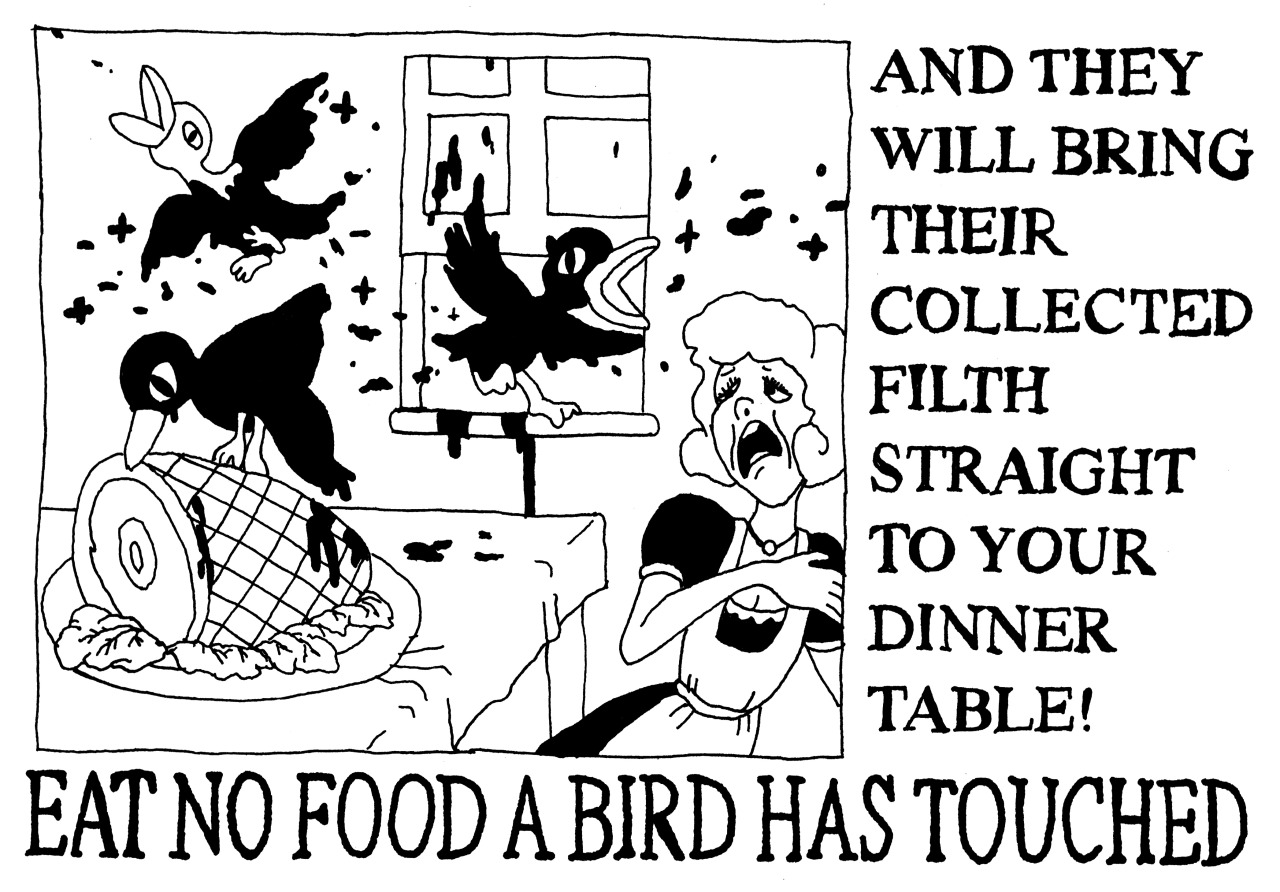
\includepdf[height=7.5in]{assets/3}

\chapter*{Wild Thing}
\addcontentsline{toc}{chapter}{Wild Thing}

%\includegraphics[width=5.33in,height=7.9899in]{media/image7.png}

I shouldn't have been here at this party. This marble fox doesn't fit in and everyone knows it. There's a group of guys just standing next to me, joking and laughing their asses off loudly. It's embarrassing that I'm so close, and yet, galaxies away from the conversation.

The room gradually shifts in red, orange, blue, yellow, and green lights. Back and forth, almost dizzying me as I stand around stupid with a cup in my paws. I don't know anyone here and my invite was done out of pity. I'd just been sitting in the cafeteria at my college when a hare mistook me for someone else and felt too ashamed to rescind the invitation.

But, I put on some nice clothes, at least, what I think is nice: Jeans and a white cargo shirt. I'm just glad I took out my fucking pocket protector before getting here. Fuck, I'm so lame. Why did I even come here if I was just gonna be sipping booze and standing alone with my tail curled around my waist.

I scan the room, thinking it might be my time to thank the host and get back to my place in the dorms. There's a stack of anime DVDs waiting for me that I've only seen a hundred times before. Watching them live their insane lives is more than enough adventure for me.

That's when I noticed him.

Another marble fox standing across the room staring at me. His eyes are piercing, the same crystal blue eyes that I have, just resting on me and me alone. At least, I think so. He could be eyeing me, waiting for me to move away from the drink table to get his own.

I shift a little to the side, his gaze following and I know for certain it's me he's looking at. Even though there's a wolf by his side, clearly talking to him as he sloshes a drink back and forth, he's more interested in me. A smirk is stuck to his muzzle and it's intimidating. He's got on a loose fitting tank top that's barely hanging off his shoulders. It's so long, covering most of his khaki shorts, that it could be described as ill-fitting if he wasn't pulling it off so well.

What sticks out the most is the flower crown on his head. I don't recognize the pedals, and they seem too large to be real. They shift colors with the lights of the room, just like the white and gray on his muzzle. A dazed look hangs in his eyes as he stares at me, and like the rest of his demeanor, he just seems so laid back and chill.

Like a Wild Thing.

His look becomes a little oppressive and I shift uncomfortably underneath it. I'm ready to just leave, scamper away from this fox that looks too cool to be interested in me, but wait! The fox says something to the wolf, dismissing himself casually as he starts towards me.

I can't think of a reason why. My glasses feel crooked on my muzzle and I adjust them like the dork I am. Trying to recover, I bring the drink in my paw up to my muzzle, and take a sip only for most of it to dribble over my chin. Why can't I do anything cool?

I brush the liquid off with the back of my wrist, probably looking worse than before but the Wild Thing just chuckles. He's sleek, wirey, flowing between the other guests like wind. His fur pattern is similar to mine, very close as it glows red, orange, blue, yellow, and green with the shifting lights.

"Hi," I let out in a whisper, and then realizing he probably can't hear me, I say too loud, "Hello!"

He keeps that same smirk and says back, just loud enough, "Hey there."

Trying at a conversation, I point up at his crown and say, "I like your flowers."

The Wild Thing nods politely and softly replies, "Thanks. I had a lot of fun making it."

There's a pause as his gaze moves from mine for the first time, taking a second to eye me up and down. I feel underdressed, but he seems to like what he's looking at. He's a little close, closer than I'm used to, but I can't get my legs to move back. With my free paw, I brush my tail around my waist to relax until it unwinds behind me.

The Wild Thing steps beside the drink table and grabs a cup. Despite all the attention flustering me a second ago, his immediate dismissal of me feels empty. He's just fixing himself a cocktail, not turning to me. It's at that moment that I realize, I'm the one staring at him now and feel a bit abashed. I should've known he wasn't interested in me.

A sudden flash of embarrassment and anger in myself strafes through my core and I decided it was time to leave. Just as my foot makes the first step towards the door, a paw grabs hold of my arm. I turn to see the Wild Thing holding me while tipping the cup into his muzzle, guzzling the liquid down audibly.

I let him hold me, his relaxed grip not too forceful, until he finishes, sitting the drink down onto the table. "If you wanna leave, I know someplace we can go," he says with alcohol fumes cascading off his breath, wrinkling my nose.

His words are so confident, without any hesitation or thought. He lets go of me and flicks his head to the side towards a hallway. I peer over him, down the dark passage he wants to lead me. Then I look back to the front door that'll take me to safety. I decide and my muzzle is drawn back to the Wild Thing.

He's so handsome, and though the other marble fox looks similar to me, he's so much more. I don't just want to be with him. I want to be him, and I want to gain a fraction of what he has just through osmosis alone. So, trying to imitate his coolness, I say, "Sure."

Without another word, he turns to the hallway and walks away. I'm left standing for a second, and only with the swish of his thick flowing tail, do I realize I'm supposed to be following. I don't even set down my drink, trying to catch up to him in large steps.

While he ambles through the bodies, men and women my age flirting with each other carelessly, I'm left awkwardly stumbling between them. An \emph{Oops, I'm Sorry} here and an \emph{Excuse Me, Pardon Me} there, I manage to just barely follow behind. It feels like there's eyes on me, not just judging my clumsiness. My head gets the better of me and I hear voices questioning how I was the one who the Wild Thing approached.

He's so out of my league, and yet, I'm the one he wants. I know, because a single eye turns back to make sure I'm following. He doesn't take the first door, like he knows where he's going. I think he might live here. Like he just plucked his prey from the crowd and was dragging it to his den. I don't mind. I'd gladly be his, if he had me.

It's the third room before he grabs the handle and twists, the door opening as silent as his footsteps. There's no lights, but the glim glow of the moon illuminates the room. He turns, inviting me in, and I feel a little comfort that he seems so eager I join him. I step inside and he doesn't hesitate to pull me into a kiss.

Both of his paws are on the collar of my shirt, stretching it as he forces his lips against mine. His claws tear at the fabric, and I'm worried for a second that he might just shred my clothes rather than let me take them off. My paws straddle his sides, holding him to steady myself as he pulls us towards a bed.

The Wild Thing sure lives up to the name I've given him, because he is after me like a beast. He lets go of my shirt just to slide a paw up underneath it and start yanking it off of me. Even as the kiss breaks momentarily to pull it over my head, he is relentlessly back to nibbling my lip.

My huffs are hard like his, our breath mixing as we tangle paws around each other. I fling his shirt to the side, my pants come off and are kicked aimlessly away. I've never done this before, but my instincts take over. It's not long before I'm down to my tighty whities and he's wearing nothing but what god gave him. And his flower crown, of course

I'm pushed backward, a worried yipe escapes my muzzle fearing I'm about to hit the floor. The soft squeak of a mattress underneath me breaks my fall and I'm left scrambling to grab the sheets. I try to hoist myself back up, but a paw lands on my chest and holds me down. I'm worried for a second this might be too rough, but the claws tracing sensually underneath the fur on my belly tells me it's exactly as rough as I'd ever wanted it. Just fast!

A warm wet tongue wraps around my length, and I lean my head back deep into the comforter. My teeth are grit, and it's all I can do to keep myself from moaning out loudly over the noise of the party. His lips draw back and forth against my cock and the warm breath of his own moans wash over me. One paw stays on my stomach, digging in lines perfectly over my sensitive spots. The other is handling my balls, rolling them around and squeezing them gently between his fingers.

He's getting me close, and it's happening too fast. I can feel him edging me towards the point of no return without even taking me in his muzzle. A hot embarrassment is flooding over my mind, not sure how to tell him to slow down or stop. Though, if I'm being honest. I desperately don't want him to slow or stop anything. Before I can though, he pulls his lips off my cock and stands to his feet.

"You should be wet enough now," he says, extending a paw for me. I'm not sure what he's talking about and I stare up at him dumbly, my brain still floating in my head.

He shakes his outstretched paw again, and I blink before taking it. I'm off the bed and he takes my spot, crawling up on all fours and holding his tail up with a paw. His backside is fully presented to me, and I realize now what I'm supposed to be doing.

"Are you sure?" I ask, already crawling up behind him.

He only gives a nod and flicks his tail from right to left. I touch the tip of my prick against his hole, the warmth sending shivers up my spine. With only my spit and pre for lube, I lean forward and enter him. A soft purr lets me know that I'm slick enough to be pleasurable.

One paw goes on his back and the other grabs his hips as I inch closer to him. My knees drag on the sheets. I can barely see him, but I don't need to. Just need to feel him; feel his hole wrapping around my cock as I push myself inside.

There's a moan of pleasure, and I'm not sure if it's me or him. Our pants and huffs become one, just over the slapping sound of my thrusts. I instinctively lean over him, fucking his ass doggy style. My paw wraps around his length and I begin pumping him to my thrusts.

Each pull and push sends waves of serotonin through my brain. His cock is slick in my grip, pre stickying my paw pads and the fur between my fingers. I dip my muzzle low, nibbling against the other marble fox's nape. A sense of pride envelopes me as I realize I, me alone, am the one taming this Wild Thing underneath.

My climax is quickly approaching, and I know his is too. He's leaking like a hose, pre covering my fur and the bed. I tighten my paw around his shaft, pumping him faster as I get close to shooting inside him. He calls out something in his moans, and I think it's my name, though I'm sure I didn't tell him that. His reward is my teeth sinking into the fur at the back of his neck. I feel his cock spurting just as I hit the point of no return.

I knock my knot against him, once, twice, three times, but the spit isn't enough to push past his ring. It doesn't matter. My eyes squeeze tight, and I orgasm right into the other fox's insides. Cum shoots deep into him, lining his rectum with my seed.

He's moaning loudly, even with me biting down hard (or because). My paw loosens, and I slump over him. The Wild Thing holds me up on his back as my balls empty into him. There's a sureness that I filled him up so much, my seed is leaking out his backside.

Carefully, he lowers himself until he's on his belly, and I let go of him just as my paw sinks into the puddle he's made. I pull out, rolling over onto the bed and taking my paw with me. It pulls free from underneath him, wiping most of his spunk onto the sheets and his fur.

With my back on the bed, I stare up to the ceiling and wonder just who I am. Maybe it's the afterglow settling in my head, but I'm feeling particularly proud of myself. I'd never imagined I could just follow a stranger into a room and have sex with them. I'd never so much as given a handjob before.

Part of me wants to ask if it was as good for him as it was for me, but that sounds stupid. Still, I should at least say something, and the only thing that comes to mind is, "That was amazing." and when I think about it, it's not the dumbest thing I'\textbackslash ve ever said.

He hasn't said anything back. I observe my surroundings, seeing a lamp on a nightstand next to me and flicking it on. It's only then that I notice it. He's laying on his side, turned away from me and I see the pattern on his back. His marble fur, gray, white, auburn, orange, and red, is so similar to mine. And there is this sun kissed patch of fur on his shoulder that is just too familiar.

Way too fucking familiar.

My heart sinks in my chest, and I realize that he's way too similar to me. I just fucked my cousin. Of course, an idiot like me would abso-fucking-lutely accidently lose his virginity to his own cousin. The taboo instantly washes over me, and dread fills my soul. Before I can think of what to do next, possibly sneak off, if not run, grab my clothes, get the fuck out of here, and avoid any family reunions for the rest of my life, he says, patiently, "I'm not your cousin."

He's not looking at me, still turned away. If he's not my cousin, then---

"I'm not a lost twin brother either."

Is he?

"---And I'm not reading your mind. Jeez, would you just settle down for a second," he says dismissively.

With a nervous smile on my muzzle, I say anyways, "If you're not reading my mind, you're not making a good case for yourself."

That's when he turns over to face me, and I finally see it. I see me. It's actually me! He's got a sly smirk slapped on his face, just as my muzzle is twisting into a frown. This cannot be happening.

"Yeah, I'm you. Just a little older," he says, reassuringly.

I study him, my eyes going down to his body. He can't be me. Not only is he missing my glasses, but he's just too perfect to be me, too calm and collected. Too amazing. He's the Wild Thing, and I'm---well, I'm just me.

"If you're who you say you are, then you'll be able to answer something I'd only know," I say, trying to think through my thoughts.

I find it; a memory that's only true to me. A little marble fox comes to mind, and I see him gathering dirt and worms to put in his elementary school teacher's purse. I was such a miscreant and I'm about ready to ask him to repeat the story, but his muzzle is pulling back wider than before. And I see it, in his eyes, the reflection of my own muzzle, pulling back at the thought of the memory.

We're reliving the experience together.

"How?" I ask, not needing any proof. Just answers.

Out of nowhere, he extends his paw for me and I see it sitting on his pads. It's a multicolored pill, shimmering in the dark of the room. He's offering it to me, and I know I'm supposed to take it. Before I reach out, I've got only one more question:

"Is it safe?"

He gives me a wink, and says, "It's worth it."

I pluck it from his paw and hold it to my eye. It radiates in red, orange, blue, yellow, and green along with every color in-between. The Wild Thing gets comfortable, resting his head on a paw patiently. His smug look tells me he knows what I'm going to do next, so I take the date with destiny, and plop it into my maw.

It doesn't taste like anything, but it does hum on my tongue. There's a slight buzz of electricity or something, and I hesitate to swallow. I consciously have to will myself to get it down, and I feel it roll against my throat. Even sitting at the bottom of my stomach, I can still fill its pulse inside me.

"Well?" I ask, expecting something to have happened by now.

The Wild Thing chuckles and says, "Oh right." Then, faster than I could have anticipated, he snatches the glasses off the bridge of my muzzle. "I wanted these back."

"Hey!" I exclaim, ready to take them off his face. Just as my arm reaches out to grab them, I watch in horror as my paw disintegrates. I stare down at where my arm used to be, jaw trembling. I turn back up to him, that smug look annoying the shit out of me. I say the only thing that comes to mind, "oh, you mother fucker---"

Reality folds in on itself, like a book being slapped shut an inch short of my nose. It becomes apparent that my body is no longer my vessel. I've been split into trillions upon trillions of atoms and the only thing that exists of me is my consciousness. I clutch desperately at anything, but with no arms and no clue of what to do, I'm just thrown about between time and space.

My thoughts are the only thing that are held together, but even thinking feels like walking miles between ideas. Time itself is lost on me as my consciousness flings through the void I exist in. I try hard, grasping to remember what I am or was or will be, putting myself back together like scooping sand on a beach. And all at once, I find my foothold.

I am born. My name is Thomas Forewind. My father, a serf, kisses me on the forehead as he lays eyes on me the first time. I'm a boy, a wolf cub, and I tend the fields with my family. I grow into quite the rambunctious teen.

With my friends, I dance at the slightest start of a beat and when I sing, it's louder than anyone else in the tavern. Anything to impress the barmaids and my friends. It's joyous for a time, and I couldn't imagine anything better than this.

There's a raid and in the span of a few hours, all of my friends and family are gone. As smoke rises from smoldering buildings, I am left orphaned, angry, and hollowed. I am asked to fight for my kingdom against these raiding neighbors, and I do so gladly.

With my shield wrapped around my arm, I clash against a leopard coming at me. He's an older man, maybe a veteran and he's confident. He swings his sword at me with precise thrusts, but I knock his blows away easily. I am good at this. He dies by the swipe of my blade, and I look for the next opponent.

Ten more come at me, one after the other, and there's ten corpses I'm left walking away from. I'm reveling in my prowess. Who'd have thought I could be a killer? I approach a fox, a boy\pagebreak\ like me. He's terrified, already seeing what I can do. The other teen throws down his sword in surrender, stumbling backwards as I approach. All I do is smile, thinking this one would be the easiest.

I raise my sword, ready to strike him on the ground, but I recognize the fear on the vulpine's muzzle. It looks like\ldots me? I realize just what I've become. I don't want to be this! I'm not Thomas Forewind! I am\ldots I was something else. This doesn't make sense, and reality falls apart again. Thomas Forewind disappears on the battlefield, and is labeled a deserter, never to be seen or heard of again.

I am tossed again in the ocean, and I feel my thoughts swimming against a current. My consciousness is thrown about, and I look for something to stand on. But without a body or any physical manifestation, it's like trying to stand on the waves itself.

I'm a skunk now. My parents name me Julia after my grandmother. I like helping people, and I'm gonna be a doctor someday. The path is so clear to me, all throughout highschool and college, and I don't waver the slightest. They put me in the ER, and I'm ready to save some lives.

But a gas leak across town causes an explosion on my first night. There's too many people coming in all at once, and the hospital is immediately overwhelmed. We're short beds, short staff, and I am made to pick who I can treat and who I can't.

A bull, barely recognizable under his singed fur, grabs my arm and begs me to help him. I can barely understand him over the dozens of screams filling the hall. This isn't right. It comes rushing back to me, and I wish it wasn't happening right now when I'm needed most. I'm not a doctor. I can't save him. I can't save anyone. The last thing I see before I'm swallowed back into oblivion is the bull's eyes staring blankly into nothing.

The only thing left of Julia is an unsolved mystery tv special of a doctor vanishing in the middle of an ER.

Again, I'm caught between the planes of reality. I feel it now though. It's not an ocean of water, but the area beneath the zero-point of space itself. The sea of gluons pass me back and forth like dough in the fingers of a baker. They rise up like bubbles to the surface, and I follow them once more to existence.

When I am young, I give myself the name Wynn. My parents think this little non-binary bear cub is going through a phase, but it sticks all throughout my life, and they learn to accept it. I am lucky. It's when I'm in the junior ranger program that I learn my first crush early: Nature.

I love it more than anything and it's enough to satisfy my needs. In the trees, the flowers, the red, orange, blue, yellow, and green of its body, do I know it cares for me as well. There's no other person for me. Its love is unrelenting and a hundred times more than what I or anyone else could ever express.

My first and last job is a park ranger, sworn to preserve nature's beauty for future generations.Though the national park program throws me all over the country, I finally settle on a green valley where the sun sets right at the end of a canyon. I take pride in my work, and even when I'm pushed into retirement, I stay closeby.

I take one last hike up the mountains, forcing my bones to make this final trek. There's a boulder I'm able to climb up, and I rest with my legs dangling over the edge. Life's been good to me, and there's no other way I would have done this. With my finishing breath, I let out a sigh and give myself back to the ether. Wynn disappears just as the sun sets.

I am once more.

And it's me this time.

I'm sitting atop of the void, floating as mere consciousness in space. The sun's warmth, even a dozen million miles away, wraps my existence in a blanket. With a level head, I see my atoms scattered through the whole of the universe.

Like a child with building blocks, I put myself back together in the recess of space. I admit, it takes me a little longer than I wanted: just a few decades of pulling piece by piece to me and stacking them on top of one another. When I get to my eyes, I can see the slight astigmatism and choose to leave it, putting each part of myself back together the way it was intended until I can see again.

As a marble fox floating in nothingness, I ponder what I've done and what I shall do next. There's a momentary flash of guilt that bubbles up. Thomas, Julia, and Wynn were all created because I couldn't find control and they lived real lives with real people, only for me to have pulled them from existence.

I'd wished the Wild Thing would have warned me, but I worry if that would've changed my decision. Instead, I have to live with and as them, taking their memories and their feelings along for the rest of my journey. But I remember me too, and I remember I had my own ambitions to fulfill.

And like a dork, the first thing I think of is to see a black hole. I'd always been fascinated with sci-fi, and imagined what it'd be like to witness one. Now, as what I've become, there's nothing holding me back. I say goodbye to my sun, giving it a small wave, before turning my attention to the galaxies beyond my own, and push myself forward.

Space and light become a blur, and I'm shot millions of light-years across the universe until I see the black hole I want. I approach it, moving through the void as easy as swimming through a pool. Planets and stars wizz past until I'm safely in viewing range of Messier-87.

It's aweing at first. I can see the acceleration disk burning brighter than anything I'd ever imagined. The raw destruction and power holds me for a few hours, but I'll tell you this: You'd not believe how fast you'd go from, "Wow, a black hole" to "Okay, black holes are kinda boring."

I clap my paws against my hips, rolling my shoulders awkwardly. Part of me feels like I need to excuse myself to be polite, but it's just a black hole. It doesn't really care how entertaining it has to be. So, I point myself to another direction, wave stupidly anyways, and I find a space bar out a few thousand years in the future to manifest myself inside.

They don't actually call it a space bar, cause that'd be dumb. It's just a bar that happens to be floating in space called Rico's Dive and Dine. Freighters stop at it to refuel and to relax between asteroid belts and planets. There's a small crowd tonight, and all stop and stare at the naked marble fox standing in the center of the room.

Oops, forgot to put together my clothes. My presence shocks some in the crowd, but a boar in a denim jacket says, "Someone's been going through Sally's personal stash again." Everyone laughs, and the big man stands from his seat at the bar to approach me.

For as large as he is, he doesn't seem to be mad nor does he try to intimidate me in any way; just holds up a paw and asks me if I'm alright. I flick my tail over my privates and nod sheepishly, the attention a little too much. He asks what I'm on, high or drunk, and I chuckle and say I'm sober. Just forgot my clothes.

Then he looks towards the entrance, trying to see if I came in with anyone. He asks me which spaceship I'm piloting or where my crew was, and I shake my head. I say, "I am my own vessel," because not only is that the truth, but it also sounds pretty badass.

That just gets another roar of laughter and they find me a table to sit at. A few come and ask me questions, but there's not many answers I can provide. I just wanted to be here and I showed up. The freight drivers manage to wrangle together some clothes for me, and now I'm wearing the loose fitting tank top and cargo shorts the Wild Thing was wearing. Destiny is unfolding in front of me.

Feeling confident, I make conversation with the crowd and learn about their worlds. They pass me drinks as I explain my journey to get here, and everyone in the bar is invested. I think about my time as Thomas, the medieval wolf, and I remember him at a tavern surrounded as such.

With the alcohol in my system, I think back at a song Thomas sang that really riled the crowd. I thump my glass and stomp my foot, setting the beat while starting the first verse. The men and women follow along, clapping their hands and cheering loud as I jump on the bar and start prancing around in my song.

The whole crowd sings along to my chorus and my heart is filled with their voices. At the end, I repeat the last lines alone and am met with an applause so loud, it shakes the entire station. Why didn't anyone tell me it could be this fun being the center of attention?

The bar settles down and I turn to small conversation with the patrons. I feel Thomas in me, no longer empty and angry; no longer the killer I imagined him to be. He's proud, but it's not him. It's me. I'm Thomas, Julia, Wynn, and the pride I feel isn't for someone else. It's for myself.

That warmth I feel inside is too much, the energy pulsating in me needing release. I hug the boar, thanking everyone for their generosity and kindness, and then turn to the universe and find a spot to land.

When I open my eyes, I've returned to earth. I'm laying on my back, the ground warm, and the desert's night air cooling my fur. I stay there, appreciating the milky way above. I can see all the stars and galaxies millions of light-years away, and peek at them like looking through a telescope.

There's two neutron stars colliding there. Over there, there's a couple of aliens performing a form of a wedding with hundreds of guests surrounding them. All around are planets and stars and civilizations, ripe for me to explore. But a hollowed metal thud of something being kicked catches my attention.

"We're stranded!" a voice cries out.

I lift up from the ground, turning my attention away from the space above and to my surroundings. There's a van sitting at the side of a road, and a group of otters are leaning against it. One's got a blunt in his muzzle, taking a hit of it before passing it to another.

"Things will work out," an otter says nonchalantly.

A girl between the two boys throws up her arms and asks, "How?"

That's my cue.

"Howdy!" I call out, walking towards them while brushing the dirt off my back and fur.

All three jump, but I don't change my gate. They're staring at me curiously, the tallest otter shifting left and right down the road. There's nothing for miles and miles. I can read his muzzle, and explain, "I just happened to land here."

They shuffle nervously, afraid of me, though all three are taller and bigger. The one holding the blunt cautiously reaches his paw forward, extending a roach for me to take. I've never done pot before, but it seems rude to refuse the offer.

I take it, inhaling little puffs before coughing my lungs out in front of the three. They laugh at that, and quickly introductions are made. Their names are Damian, Ross, and Tiara, and their van gave out between concerts. Smoke is still pouring from the grill and I offer to take a look.

Careful with the hood, I pop it open and poke my head inside. I'm not an expert at cars, but I think I know the problem. Sensing the vehicle and seeing through its design, I can almost feel where the radiator is cracked. It's like an itch on my skin, and I mend it closed with my will until it is whole again.

The otters can't see what I'm doing, but I can feel the car heal itself. Then I draw from the air, filling the tank with water, and in an instant, the insides feel new again. I close the hood and smile at the group, a sense of relief washing over me. All is right.

I clap my paws together and say, "That should do it."

Tiara, ever the skeptic, laughs and says, "You didn't do anything."

I shrug, not needing her to understand. "Where we headed?" I ask casually.

Damian, the tallest otter, gets in the front seat and turns the ignition. The car comes back to life, and he lets out a gasp, "Well, shit." He stares at the panels, squinting as he notices the vans running better than it ever had before. Again, I shrug.

Ross, slapping a paw to my back, takes a hit and when he exhales, he says, "And the universe provides."

So I had.

I learn that I've landed in the middle of the 80's. We spend months on the road, traveling between venues and concerts and bars. Sometimes we're there to play a gig, and sometimes we're just there to watch. All these bands I only knew from the radio were now playing live in front of me, testing their sounds.

Some are met with roaring crowds, screaming out for more. Others are booed and mocked, the music not appreciated at the time. I recognize some of the ones that would later be hits, sleepers that just needed the right moment to shine. It was still good to listen to them in their raw impact.

It is with Tiara that I learn how to braid flowers into a crown. She teaches me her way of explaining she likes me. Despite that, it's Ross who is my first kiss amongst the three. He sneaks it in after shotgunning me with a breath of weed, our lips too close and our attraction too strong not to finish closing the gap.

We make out in our hotel room, one of the few times we ever get one. Tiara and Damian are out at the bar, but me and Ross had opted to stay inside for the night. I'm glad, because I've wanted this for a while.

When he breaks from the kiss, he says, "I'm sorry. I guess I'm pretty high." He turns his head away bashfully, looking to get up off the bed. I don't let him, holding onto his paw and keeping him there. Then I steal his blunt from him, placing it on an ashtray and give him a kiss on his neck.

He shudders underneath me, my teeth sinking softly into his fur. I hear him drag his claws on the sheets, muttering moans. Our clothes come off until we're down to our underwear. He's a little unsure of himself, but I know well enough for the both of us.

"Let's start slow," I say, and he nods up and down.

There's a little pudge over his front that I trace a claw through, and he likes that. He's careful when he touches me back, not wanting to move too fast. His fingers run through the fur on my chest, and I moan to let him know it feels good.

His cock tents up his boxers, and I dare a touch. I put my index finger to the tip, stroking it up and down over the fabric. It twitches and a bead of pre drips through to sticky my paw pads. He lets out a soothing purr as I pull back the underwear until his cock slips through the slit.

While I'm playing with his cock, he's more invested in my nipples. He keeps making a circular motion around them, every few seconds giving one a gentle pinch before moving onto the next. Then he dips his muzzle down and starts nibbling on me between his teeth.

The sensations are so amazing and my cock feels restrained in my underwear. I pull my briefs down, letting my cock hang out, pre dribbling freely along my shaft. Ross looks down, sees my cock, and cautiously wraps his paw around it, squeezing me at my knot.

I huff, grabbing hold of his own stiff member to give him a squeeze as well. Side by side on the bed, we jerk each other off. Together, we pant, only silenced when we're nibbling and pecking each other between our strokes. As I'm getting close, I rest my nose into his neck, breathing in his scent sharply.

He's first to cum, spraying a line of jizz across his chest and belly. I don't last a second after, and I am showered in my own spunk as well. Together, we fall back onto the bed and nuzzle in our afterglow. We stay there for a while, and I cuddle up against his side.

"I've never done that with another guy before," he admits.

I silence him with another kiss, reassuring him with my love. He feels safe beside me, and Ross doesn't even flinch when the door to our hotel opens up. Damian and Tiara slip in, pausing for a second when they see us spent on the bed together.

Even though we're in our underwear, we're still covered in our cum and it's pretty obvious what we just did. Tiara's muzzle turns, but all she has to add is, "Boys."

Her jealousy lasts maybe a week at most, before I catch her alone with a flower crown I braided just for her. Damian, ever the most relaxed of the three, goes with the flow, not denying the inevitable before we're all pulled into a foursome almost every night on the road. It seemed like they only needed me to bridge their sexual frustrations.

It's about a year down the line that I'm laying over Damian's chest, naked and panting in the back of their van. Tiara slides off of my spent cock, and turns to curl against my belly. Ross is sleepy eyed in his afterglow, his cum still fresh on my breath.

I smile at all of them, my first true friends. That warm glow fills me again, and even though I'm strong enough now to extinguish it, I know it's my time. There's a vast universe out for me to explore, and this is just a fraction of what I can experience. It's left an itch under my fur, and though I'll miss them greatly, I know they'll be fine without me.

"I love you all, \emph{so much}," I say, and stress that last bit just so they understand. There's a small hope that one of them might recognize what I'm saying and tell me to stay. If they'd ask, I know I'd never have the willpower to leave. All they do is chuckle, and pass me love yous as well. Carefully, I stroke them all in the back of the van, trying to hold onto the touch of their fur. It's important that I remember this and find a place in my heart to cherish it forever.

And then I'm gone.

For a while, I travel here and there. Sometimes earth, but most times not. Sometimes with friends and lovers, and some eons I'm left in quiet solidarity to explore the stretches of the universe alone. It's only when I come back to Messier-87, do I remember something important.

I remember that awkward wave I gave it so long ago, remember how this all started, and see myself so young and new. I've got business to do and I need to get back to that party. But first, I've got to pick something up. Something that isn't mine.

Again, I give an awkward wave to the black hole, feeling our time was short, and again, it doesn't have to impress me. It's a freakin black hole. It couldn't give a shit.

Then I find myself far into the future. I see a gas giant orbited by a hundred thousand railguns. Hiding in the planet's ring is a top secret station; a research facility where they're developing the pill I need to give to myself. There's a room where it's being held in and I can't just manifest into it. They've shielded it from me, or whatever threat they perceived I might have been, keeping me from stealing what they've worked so hard to achieve.

Sure I could spend a millenia researching it on my own, but that's not how it went down or how it will go down. Oh, don't think less of me for being a thief. They're Nazis. Space Nazis! Yeah, that's right, they come back and this thing they've created is to ensure their dominance over the universe. I can't let them have it.

I will myself into the station, standing outside a hallway alone. But I'm not alone. Time stretches in front of me, and I see the few infinite versions of me standing in front of the door. I am seeing every future of me making the decision that'll change all of time.

I watch as each version turns back to greet the one behind. Three ahead, the marble fox goes for a wave. Two, the next one gives me a sly smile. The one directly in front of me turns back, and I recognize that mother fucker anywhere. He gives me a wink, and there's no hard feelings between us. I turn back, seeing a couple infinite marble foxes standing in a row behind me. With confidence, I give mine a thumbs up. In turn, that one shows me up by giving his me a double thumbs up.

He's the fun one, I can tell.

Then I look forward and see that all the me's have turned their heads to the right. I follow suit, glancing into a passage of time beside me. It is there, I see a road that has never been taken, but exists all the same. It's a reality where I don't get my paws on that pill. An existence so dark and bleak, both in past, present, and future, that it proves one thing certain: I always stop them. Every time.

The me's collapse into one and I push forward on the double doors leading into a hallway in the research station. There are lizards of all sorts, each wearing white lab coats and visors. They're scrambling, the time of their ascension dawning, and none of them look up from their tablets and notes to notice a fox wearing a tank top just waltzing in.

I am fast and small, walking behind and between the men and women. At some points, I pause, waiting for a group to pass and others, I hurry by quickly. My timing is perfect, because it has to be. It's almost crazy to think, with all the railguns and high tech sensors and the room I cannot penetrate, not a one thought to lock the front door.

Ahead of me, there's a metal corridor ceiling with lights flashing above. There's a tall komodo dragon walking with a couple armed guards at either of his side. He's moving with a sense of authority, chest out, shoulders straight, and his head tilting back so no one could be at eye level with him. Even amongst his own kind, he thinks himself above everyone else.

I get close behind the dictator, the guards stopping just at the door and taking either side of it. They turn and to about-face, but their movements are so formal that neither even notices me walking just underneath their line of sight.

I stop in the room, pulling my tail forward just as the metal door behind me is sealed shut. The komodo dragon walks to a table in the center of the room, and I see the pill, shimmering in red, orange, blue, yellow, and green, along with every color in-between.

He steps around the table, getting into a position that I think he imagines to be more dignified or something. Just before he gets to his moment of triumph, he notices me across from him. He stares for a minute, blinking a couple times as if I might be something caught in his eye.

The tyrant looks around, as if I were a prank his subjects were playing on him, and at any second they'd come bursting in saying surprise! No one is coming out, and so he asks in his final question, "Vhat iz dis?"

I raise my paw, feeling energy coursing through me before releasing it out directly into his chest. In a flash, the komodo dragon is nothing but a spray of blood and ash against the wall he was formerly standing in front of. I'm a little stunned--- no, a lot, because I wasn't expecting that to happen at all.

In my head, I pictured him crashing into the wall and falling unconscious. Then I'd take the pill and he would wake up, shaking a fist in anger as I foil his plans for galaxy domination. Nope, he is very very dead, and I probably should have tested my powers before this point.

Oh well. If anything, that was a freebie.

I snatch the pill off the table, clutching it in my paw and squeezing it tightly. Unlike the fascists, I know this is too valuable to leave somewhere it can be stolen. Instead, I place it deep into a fold between time and space, ever to be locked away until I need it once more.

My work here done, I look out towards earth, willing myself to sail back home. With a thud, I smack muzzle first into a wall in the room instead. I'd forgotten that this is the one place I can't travel through. That was embarrassing. Even as a demigod, I can't help but look like a massive dork.

With a sigh, I walk back to the sealed door and give it a knock in succession to a tune I remember. It takes a second before the metal room opens up and the two guards greet me in shock. I take a step outside right between the two men. They both raise their guns at the same time, ready to empty their clips inside of me, but I'm already gone, and they only end up eliminating each other and any proof of my existence.

Invisible, atop of a railgun is where I place myself after. I sit there, watching their society from afar. They conclude that their experiment was a failure and never attempt to recreate it again. For as strong of a civilization they were, all that talk of master species and unity falls apart with their charismatic dictator gone.

Quickly, even before they finish cleaning off the bloody wall of their once great leader, factions are being made. Arguments of what to do next and how to conquer the galaxy falls to infighting. They splinter and a great civil war happens. The railguns once meant for me, are now turning on one another.

I picked a good one, it lasting most of the war. The reactor inside hums, vibrating the barrel underneath me. Radiation leaking from the core turns the whole thing blue, and just before it can get too hot, the barrel erupts. A projectile launches from its tip, racing at unfathomable speeds to eviscerate ships, battle stations, and other railguns thousands of miles away.

The war lasts years, and I feel a little guilt that I caused this. I didn't want this violence, but I couldn't just let them go through with their plans. It felt like the only option at the time, but I wonder how I could have changed things. Before I can ponder it too hard, I see something coming out the corner of my eye.

It's a bullet from another railgun. I slow time, and even as seconds get stretched to months, it's almost moving too fast for me to follow along. Gradually, I rise from the barrel, stepping off into space just as the hull is pierced through and through. An azure glow spills from the reactor, leaking into space, and the whole gun lazily spirals into nothing.

Decades pass and the war is over. I stay close by, watching their society in fast motion. They rebuild, not just their crumbled buildings and their ruined stations, but they find their heart amongst the destruction. Their war has left them tired of fighting, tired of dictators, charismatic leaders, and talks of power and ruling the galaxy.

I watch a freighter come for the railgun, pulling it into pieces. What is salvaged of the core is sent millions of miles away to power a station's garden atrium for generations to come. The barrel is chopped to bits, and I follow a small section smelted into raw metal that is later repurposed.

At the end of its journey, I see a small komodo dragon hatchling, unwrapping a present and looking up at his parents in pure bliss. He'd never know that the casing surrounding his little easy bake oven was once a tool of awful destruction, and everyone's better for that. I leave, knowing there's nothing left for me to see here.

I've got a party to go to.

I think to just show up, but that feels a little rude. No, I need a proper invite. Then I remember the wolf the Wild Thing was standing next to, and I chase after his image through time and space. It's kinda hard to flip through a trillion muzzles in history, but I eventually land on him about six months before the party.

I catch him in a green coffee uniform, during the middle of his break. He's sipping on a latte while flicking through his social media feed, and seeing him in the light, I realize just how handsome he is. It intimidates me for a second. For all the lovers and all the adventures, he catches me a little off guard.

Wiggling my body until I'm feeling loosey goosey, I give my muzzle a slap and tell myself to get it together. With some bravery, I jump right into it, walking into the cafe and taking the seat across from his table to introduce myself. The wolf's name is Giovanni.

He's a college dropout, living in a tiny apartment in a shitty neighborhood on the outskirts of town. When he's not playing video games, he is writing poetry, but he's mostly playing video games. Don't look down on him because I love nothing more than spending time together. When we go out, he likes burgers and hates sushi, but he does it for me anyways.

Giovanni is saving himself for someone special, and I know it's me. I know because I look far into the future, when his fur is gray and his eyes are milky. No spoilers. Just a quick peek, right? Even though he can't see me so well, he recognizes me walking into the room and says, "Hey Handsome, I love you."

He doesn't say it because he knows what's about to happen next. It's just something he likes to do spontaneously, and he genuinely means it every time. It makes me feel good, that same warmth coursing through my body whenever he tells it to me, and maybe that's why I'm just a little too distracted to notice. I don't see the clot building up inside his head until it's too late. I say I love you back, and before anything can be done, he's gone.

I am cold, scared, lost, and utterly alone.

"Are you crying?" Giovanni asks, and I shake myself from my vision.

I'm not alone; I'm sitting cross-legged on his couch with a controller in my paw. We're still just playing video games together in our youth. Giovanni's got a concerned look on his muzzle, pausing the screen for a second to check up on me. I wipe my eyes and nose with the fur on the back of my wrist.

"Yeah, sorry. Allergies, am I right?" I say, nodding assuredly.

He leans his head back, a sly smile on his muzzle as he stretches out a, "Surrrreee," unconvinced.

I shove him with my shoulder, and though he's almost a foot taller than me, he shoves me back just as hard! The big bad wolf. We're laughing, and resume playing the game. He'd give me so much shit if he knew I was crying about an ending. It was always about the journey. I should know that, better than anyone else.

He goes back to telling me about this cool party, and he wants me to be his plus one. Giovanni is so close to asking me out, but he's not quite there yet. This is just a way to spend more time with me, and I shield the rest of our future together from myself. When he finally does ask me out, I want it to be a real surprise.

But if he's not gonna do it tonight then I'm gonna get it from somewhere and I know exactly from who. I tell him yes, but I need to stop off somewhere first. No homo, so we fist bump before I walk out the door and find the last thing I need.

Sitting on a building sized tree at the end of the cretaceous period, I string together a bundle of flamingo pink flowers. I watch the sunrise, taking in the vast greenery of lands untouched. There's a brachiosaurus taking a bite of the leaves next to me, and I reach out to scratch its long neck.

It likes the attention well enough, even if it doesn't know what to make of me. This time and place feels good, and I realize that the Wild Thing was right all along: I am having a lot of fun making this crown. At this point, even after all this time, I finally relax and accept that he was always me and I was always him.

Looking up, I see an asteroid approaching. It's coming and I fold my ears back in sorrow. There's a thought that I can stop this. If there is any time I can play god, it's right now. But I know it's not my place to do anything, and I know that party isn't gonna happen if I make any big changes. I'm not god. I am the Wild Thing.

The asteroid slams into the planet, the blinding light of a hundred million megaton explosion sets the world ablaze. I give a final pat to the brachiosaurus, the creature running for its life away from the destruction. As the ground tremors up towards me, I take a bow, and I'm back in front of Giovanni's place.

He answers the door and compliments my flower crown. Just for fun, I tell him it's not half as beautiful as he is. The wolf's muzzle turns red, but he pushes past it and holds up his phone. The rideshare is coming, ready to take me the last mile towards destiny.

When the front door opens, it's the hare that invited me to the party. He greets Giovanni with a side hug and then the wolf turns to introduce me as his plus one. The lapine looks at me with some confusion, recognizing me, but I'm just the loner he accidentally invited to the party. Thankfully, he doesn't put too much thought into it, and welcomes me inside.

I spend most of the party with Giovanni being introduced to his friends. They're all chill, and it's not too hard to have a good time with them. But it's a little difficult to also not be so excited, and I've got to focus on the conversations, hoping to make a good impression on his friends.

But it happens.

Standing across the room, holding onto a cup for dear life, I see me. It's hard to not break down into tears. There I am, a thousand years younger, and the second biggest dork in the whole universe. And my heart is filled with so much pride.

He's here. He showed up. I can see him more clearly than he could ever see himself, and I'm just so god damn proud of him. It's a Friday night, and though he could have spent the evening watching animes he's seen a billion times over, he's chosen to step out of his comfort zone for the first time.

He doesn't have a single friend here, but he came anyway with the hope to make some. The invite was out of pity, but he dressed nice and remembered to take the fucking pocket protector out of his shirt before showing up. This night could have been disastrous, and though he doesn't have my powers to see into the future, he went out anyways, like a real champ.

He's flawless.

In my opinion, that's the reason why he's so much cooler than me. It's what makes me feel this intense attraction to him, and I'm getting a little hot and bothered. The marble fox across the room is slender, young, and so nervous. He has nothing to fear, because anyone would be so lucky to be with someone as special as he is.

That's when he turns to me, and we make eye contact. I remember my thoughts; see what he thinks of me, and I'm flattered. In his mind, I see me as true: I am the Wild Thing, and I want to be with him as much as he wants to be with me. Except this time, I think I'd like to be on bottom.

\cleartoverso
\includepdf[height=7.5in]{assets/8}

\chapter*{Cut}
\addcontentsline{toc}{chapter}{Cut}

%\includegraphics[width=5.23702in,height=7.84531in]{media/image10.png}

Dante rose up and down, gasping every time he felt the wolf's knot knock against his backside. Seven inches of cock was deep inside the opossum's ass, touching against his prostate. His own shaft was wrapped in his paw, stroking it up and down tightly. Beads of pre rolled down the side of his length just like the sweat dripping from his brow.

The room was hot, even with the lights off and the curtains drawn to hide the two from the sunlight. A ceiling fan overhead did nothing but swirl around the warm air and the scent of their pheromones. Their moans of pleasure rang just above the sound of the squeaking mattress and rail line screaming in the distance. Everything felt sticky, but it didn't bother Dante. He just needed release.

"Aww shit. Fuck man, I'm---" the wolf cried out, sinking the back of his head into the pillow it rested on.

Dante felt the wolf's claws gripping tightly against his sides. They dug in deep, but not hard enough to pierce his flesh. He continued to ride the wolf, pumping his own cock to get himself there as well. Even when he felt hot cum shooting in his ass, he wasn't anywhere near close to finishing.

Gradually, the wolf slowed his thrusts as his orgasm leaked into the opossum's backside. Warm spunk filled his rectum and dripped out his hole. The lupine knot pulsated against him with every new squirt that filled him. His ring was wrapped tight around the shaft, milking the last of his climax.

"Ah," the wolf gasped, giving light pats at Dante's sides. "Too much."

The opossum wasn't close and he knew that the wolf was becoming overstimulated as he tried to continue riding him. With a sigh, Dante pulled himself off, watching the other man's muzzle scrunch up and his eyes cross. He felt the cock slide out of him with a slurp before the tip released, his dick going limp with a plap.

Dante laid himself on the bed, dick still twitching. Part of him wanted to finish beating himself off, but instead he just curled at the wolf's side. He wrapped his paws around an arm and cuddled in close. At the very least, he just wanted to hold onto someone. If he could have that, then at least something would go right.

"Um, Dante, right?" the wolf muttered out, not facing him.

"Mhm?" he mumbled, closing his eyes and taking in the wolf's scent.

The lupine paused, thinking over his words a second before saying, "You're kinda warm."

Dante sighed again, figuring this would happen. Carefully, he unwrapped himself off the wolf and got an inch away from him on the bed. "Yeah, just kinda hoped we could cuddle a bit."

The wolf nodded his head, but remained silent for a minute. They laid there for a few minutes, the wolf getting bored, patting his paws to his hips to entertain himself. Dante got the hint, his dick already softening as he pulled off the mattress. Before he completely gave up though, he asked, "Do you wanna go catch a movie or something? The new Doug Riot film is coming out and I wanted to see it."

Again, the wolf stayed silent for a second. Dante could practically read his mind, seeing his eyes searching for excuses. He had to keep his hopes up, even when he knew the answer.

"Actually, ugh, I kinda had plans tonight. Do you need me to order you a ride share, or\ldots" he said, stretching out the last word long as he waited to be interrupted.

"No, no. That's fine," Dante said, trying not to sound as pitiful as he felt.

They rolled off the bed, Dante finding his clothes scattered around the room. There were piles of clothes the wolf had left out, settled next to equally revolting bags of trash. It was the red flags he blinded himself from in the heat of the moment. Somehow, he'd thought this hookup would have gone differently.

"My ride is here," Dante said, standing by the front door. He flipped his smartphone in his paw, looking down at the ride share app. There was a thought to close it and ask for his number. No, he wouldn't do that.

The wolf was seated on his couch, not even bothering getting up. "Alright. Um, sorry about, ugh, the whole thing. I'm usually not that fast."

Dante nodded, mostly for the wolf. Then, with his shoulders slumped, he left. Tears welled up at the sides of his eyes, but he didn't let them fall. Instead, he just kept his muzzle lifted and stepped down the porch and across the walkway. There, at the end, was a tiny red car waiting for him.

He took a spot in the backseat, not even bothering to buckle up his seatbelt. Immediately the driver began speaking, "No, I do not know where you left Mom's bracelet. Did you check in her jewelry box by the mirror?"

Dante lifted his head, asking, "I'm sorry?"

The raccoon shook a paw backwards, giving him a couple shushes before pointing at his headset. Dante rolled his eyes and tucked himself into his seat. He had set the destination for his house, though it was the last place he wanted to go. All that was waiting for him was his shelves of movies and a room he needed to fill.

Thinking about that, he pulled out his smartphone and brought up the wanted ads. He had looked through his post looking for a new roommate, but there were no responses yet. It'd only been a week since he made the ad, but he didn't have much time left. If he couldn't find a replacement for his roommate, then he wouldn't be able to cover the rent on his own.

Then he'd be evicted, which would just add to the list of problems he was already dealing with.

Dante sighed, closing the phone for a second and looked over the rest of the car. It was sterile clean with a bottle of water in front of him. He was ready to reach for it when he noticed a note above it. There was a dollar bill scribbled onto a paper and a little bag for cash.

Figures.

He was thirsty, but not enough to pay a dollar for a bottle of water. Not that he'd have the cash for it anyways. Money was tight already, and he had no room for even the slightest luxuries. This day just couldn't get any worse.

His head leaned to the side, and that's when he noticed something on the seat. The opossum did a double-take, almost certain that he hadn't seen it before. He tried picturing through his memories, but he hadn't remembered there being a bundled stack of papers sitting next to him when he got into the car.

"Um, sir, is this---"

"Hush, hush, hush," the driver said, waving his paw back again before continuing his conversation with the headset.

Dante's ears folded back, not liking the raccoon's attitude. He was for surely going to give him a one star at the end of the ride. Before he could let himself get distracted again though, he looked back to the papers.

Despite not liking touching a stranger's things, something about the papers drew him forward.

Curiously, he reached out and picked it up. The front was blank, with no title or credit. He flipped open the first page and began to read the writing. It was nonsensical at the start, talking about someone's first experience seeing light. There were words being spoken to him that the protagonist couldn't understand. It all seemed strange.

The opossum flipped through the pages, landing at a spot in the middle and reading the words: \emph{Dante looked over at Rachel, his brow furrowed. She had handed him a flower, but he didn't know what to make of it. The little vixen tried thrusting the gift forward, but the small boy wasn't having it. Instead, he pushed her away and ran far across the playground to sit alone.}

Dante's heart clenched in his chest. He remembered that exact moment. Rachel was just trying to be nice, but he was so socially awkward at that age, he didn't know how to accept it. The cringe of reliving the experience had jarred him a little, but not nearly as much of the dread of someone having written down a fragment of his life.

He tossed the papers back onto the seat, heart racing as he shouted, "The fuck is this?"

The raccoon, stopped at a red light, practically swung his whole body around and growled back, "Sir, I have been really patient with you, but I am trying to have an important conversation. If you would please remain seated and silent, we are almost to your destination."

Dante threw his arms up and tried pointing to the papers. "But---"

"Sir, I am asking--- no, not you. I am working right now," he said, trying to split his attention between his phone call and Dante. The honk of a horn blared out behind them, and the raccoon turned his muzzle back to the road. The light had changed green.

The driver hit the gas, returning to his phone call and ignoring Dante still trying to signal him. When he wasn't going to get the raccoon's attention, he slumped back into his seat. His eyes turned towards the papers sitting on the seat. With some caution, he grabbed them once more and flipped the pages open.

\emph{Knowing that he couldn't get the driver to explain the mysterious script sitting next to him, he reluctantly began reading again. The car continued on through the streets, passing over tracks that bumped the vehicle enough to shake the whole car. Dante's small wire frame bounced with the vehicle, and he glared up at the driver as if to tell him to drive more---}

At that moment, the car skipped over the tracks, shaking Dante enough to make him lose his spot in the script. He glared up at the driver in annoyance, wishing he wouldn't go so fast over the rail tracks. His maw opened, as if to say something, but the raccoon was still loudly in an argument with his phone. It was only at that small moment of clarity did he realize that he was reading his life unfolding in front of him.

His eyes went back down to the paper, a lump stuck inside of his throat. Every pump of blood running through his veins could be heard between his ears. He gulped, terrified, but not able to keep himself from reading the next passage. Where was this going?

\emph{Dante couldn't take his eyes off the text. It terrified him like nothing else in his entire life. If only he had stopped reading and looked at the road ahead, he would have seen the car barreling towards the intersection. The driver in the other vehicle clearly hadn't noticed his light was red. Not even the raccoon noticed it, too invested in his phone call and not the road. The last thing Dante said before the vehicle collided into his door frame was, "Holy Shit!"}

Time slowed down. Dante lifted his head, turning it to the right with his breath held. He saw the headlights pointed directly at him, the truck mere feet away from his door. With a quick gasp, he opened his mouth and muttered, "Son of a bitch!"

"CUT!!!"

Dante ducked across the backseat, trying to protect himself from the impending crash. The opossum's entire body crumbled on itself, tail wrapped around his waist. He laid there, frozen and unable to move. Seconds stretched like hours waiting for the truck to ram into his side. Then, after what seemed an eternity, he realized nothing was happening.

His ears unfolded, an eerie silence about the car. Gradually, he began to uncurl, and lift himself off of the seat. He turned his head upward, looking at the door, only to notice that it was missing. Not destroyed or ripped off from an accident. Just gone.

The vehicle about to run into him was frozen in time, stopped mere inches from his side. He could clearly make out the driver, a husky whose face was stopped in shock. Dante could see a phone in his paw, but when he got a closer look, it was just above his fingers, stuck mid air.

"Hello?" the opossum asked, looking at his driver.

The raccoon was frozen as well, still in the middle of a sentence, completely oblivious to the crash he narrowly dodged. Dante crawled up towards the center armrest, reaching forward and poking the driver. He wobbled slightly, but otherwise was unresponsive. Just remained seated, lips midword his conversation.

"Dante!"

He turned towards the voice, peering outside of the vehicle. It was then that he realized the entire world was stalled in the second before the crash. Cars were all stuck in place, men and women frozen midstep, and even the birds were trapped in the air. All except a feline storming his way to the car.

He wore striped slacks held up by two thick yellow suspenders. The cat had a white button-up shirt with the long sleeves rolled up either arm. He carried a megaphone in his paw, waving it about as he worked his way onto the street. A black director's cap sat atop his head.

"Wrong," he said, waving his arms. "That's not the line, Dante. You've never messed up a line before."

Dante poked through the door of the car, only now realizing there was a camera rigged to the side. He looked down, realizing that the vehicle itself was on tracks. Seeing the truck that was about to hit him, he realized that too was on tracks. There was another camera hooked up to the back, a doberman seated behind it with a cardboard cup in his paw. He sipped on it, eyes half glazed as if he was bored.

"Who-- What is this?" Dante asked, looking at him. It was only now that he realized there were a dozen or so people still able to move, going about with headsets and clipboards.

The feline snapped his fingers at a mouse walking across his path, "You! Intern. Where's his script? Pass it to me."

The mouse jumped, flipping through a dozen sheets before chittering, "I, um, I uh, it's not, uh---"

"---Doesn't matter. I know the line. Dante," the cat said, getting close to the opossum. He wrapped an arm around the small marsupial's shoulder. "The line is \emph{Holy Shit}. Just before the car hits your side, you say \emph{Holy Shit}. I wrote that one specifically for you."

Dante, still confused at everything, tried asking again, "Who are you? Why is everything frozen?"

The cat shook his head back and forth, pushing Dante back into the car. "Don't worry about it. Just remember your line and say it right. It's gonna be perfect." Then he clapped his paws in the air, turning to the rest of the crew. "Alright everybody! Back from the top."

Before Dante could ask another question, the car began rolling backwards. He let out a squeak, turning up to the driver. The raccoon's lips began to move again, words coming out backwards. Everything in the world began rewinding, faster and faster until---

Dante blinked. He stared blankly in front of him at the sheet with the dollar bill.

Figures.

He was thirsty, but not enough to pay a dollar for a bottle of water. Not that he'd have the cash for it anyways. Money was tight already, and he had no room for even the slightest luxuries. This day just couldn't get any worse.

His head leaned to the side, and that's when he noticed something on the seat. The opossum did a double-take, almost certain that he hadn't seen it before. He tried thinking through his memories, and then remembered the stack of papers left on the seat next to him.

Dante was sure that he remembered something, but not what. A sense of deja-vu flooded him, and he looked over to the raccoon. Something was familiar about this, more so than the hundreds of similar rideshares he'd taken before. Leaning forward, he asked, "Um, sir, is this---"

"Hush, hush, hush," the driver said, waving his paw back again before continuing his conversation with the headset.

Again, Dante was given this eerie sense that he'd done this all before. Curiously, he reached over to the sheets and picked them up. It was blank on the front, no title or credits. He flipped open the first page, reading the nonsensical words describing someone's first experience seeing light.

Carefully, he flipped through the pages until he landed on a section that detailed an experience where he was given a flower. It was all coming back to him in pieces, and he turned towards the end, where he was sure he had left off.

At that moment, the car skipped over the tracks, shaking Dante enough to make him lose his spot in the script. He glared up at the driver in annoyance, wishing he wouldn't go so fast over the rail tracks. His maw opened, as if to say something, but the raccoon was still loudly in an argument with his phone. It was only at that small moment of clarity did he remember exactly what was going to happen next.

His eyes went up, his head turning towards the side just as he saw the truck blaring into the intersection. Just as its headlights pointed directly at him, Dante shouted, "Not again!"

"CUT!!!!!"

Dante, once more, had curled along the backseat, bracing himself for the impact. Only after moments of huddling in fear, did he gradually pull himself from his seat. That's when he noticed the car door missing again. He could see the husky frozen in fear, phone hovering just a few inches above his paw. The world had stopped.

"The fuck?!?" Dante shouted, jumping out of the car and spinning around himself. He looked left and right, noticing the camera men and women all relaxed in their spots. Interns raced around the place just as the cat pushed his way through them.

"Again? Dante, baby, what's going on?" The feline said, snapping his fingers towards the same mouse with a clipboard. "You, get him a water bottle. It's hot today."

The mouse's feet skipped off the floor and he raced towards a table full of concessions. The cat let out a hiss as he eyed a dog grabbing a bagel from a bowl. "Hey, you! That's for the talent. Is your talent eating things that aren't yours? Stay away from those!" The shepherd dropped the bagel, quickly skittering out of view.

Dante pushed the cat off of him, his mind racing as he tried to grasp everything. The sight of the completely frozen world around him was unsettling. Heart thumping in his chest, he started off away from the crew members and cat. He heard the feline call out behind, "No, Dante! Not that way!"

The opossum ran up towards the street opposite of the vehicle that was going to hit him. He knew his house wasn't too far from where he was, recognizing some of the landmarks. Full speed, he got right up to the sidewalk before crashing into something invisible. His muzzle went face first into it, knocking him backwards.

He fell hard on his ass, tail pinched beneath him. Dante scowled before looking to see what he'd run into. It wasn't invisible. In fact, it was anything but. The wall he collided into warbled, the street in front of him distorting as waves rippled where he crashed. There was no street, but instead, a backdrop of one that only looked real.

The cat and mouse caught up to Dante's side, each helping him off the ground. "Hey, careful guy. Don't want you destroying my set. Gonna rip a hole straight through reality," the feline said with a chuckle, patting dust off of his back and rump.

The mouse pushed a glass water bottle into Dante's paws before taking a step away. He stared at it in confusion just as the cat placed a paw on his back and said "Dante. Baby. Hunny. My guy. What's going on with you today? You've never had an off day like this."

Immediately, the opossum jerked away from the cat and asked, "What is going on? What is this?" His paws flailed about, the bottle in his paw sloshing around.

"What is this? What do you think it is? It's your life, buddy, playing out the way it's supposed to. Well, usually," the cat said, pushing him gently back towards the car. "Haven't had a fuckup like this in millennia.This is your big moment and everyone's waiting for you."

Dante let himself get led back to the vehicle, noticing the set around him. The people still able to move stuck out obviously now, all seeming to be wandering around. "Who are these people? And who are you?"

The cat waved his megaphone around aimlessly as he said, "Who am I? Jeez, nobody reads the credits nowadays! I'm The Director. I'm in charge of making this all work perfectly. Your life from start to spectacular finish. Again, usually. You've gone and messed up two takes now. Right at the finale!"

Dante was almost back to the open side door when his feet skittered against the asphalt. He stopped himself, refusing to go any further. "Messed up? Messed Up? YOU WERE ABOUT TO HIT ME WITH A MOVING CAR!!!"

The Director, not seeming too phased, shrugged his shoulders and said, "Yeah, that's the scene. So long as you get your lines right."

Frantic, Dante looked into the back seat of the vehicle and saw the papers thrown about. He reached inside, grabbing them and then waved them towards the feline. "Change it! Change my script!" he demanded, fangs bared out.

The cat looked at the papers in confusion before his brow raised. "What're you doing with that?" He swiped to grab it, but Dante pulled it away from his grasp. "Give it to me, right now," he said, holding his paw out expectantly.

Dante shook his head, keeping it close to his chest. "Not until you promise to change it. I'm not gonna get hit by a car," he said, getting in a defensive position.

The Director sighed while shaking his head. "No, I'm not changing anything. This is how it's supposed to go. Everyone has their purpose and we're not doing any more rewrites." Exasperated, the feline pointed to the husky, still frozen in the driver seat of his vehicle. "Look at Scott. He's terrified, but exactly where he's supposed to be. We all have a job here."

Then he pointed at the raccoon in the front seat of the rideshare. "Julian is supposed to be working out his mother's bequeathment. I'm supposed to be directing this scene. "Then he pointed to the mouse who'd been by his side the entire time. "This chucklefuck is supposed to lose your script, apparently," he said before finally pointing at Dante, "And you're supposed to get hit by a car."

The Director finished by waving at the inside of the vehicle again, like his point had been made. They stood there a second, waiting for the other to budge. Dante was the first to speak, looking back at destiny before turning to the feline and saying, "No."

The Director's eyes squinted and his brow furrowed. He could see the hackles on the cat's neck rise before he took a breath and pointed to Dante. "Take the script from him, and get him back in that car," he ordered, turning his attention to the mouse.

Dante took a step back, the glass water bottle in one paw; the script in the other. The mouse stepped forward with very little confidence. He held up his own clipboard and stammered out, "Ugh, please, um, would you hand that over and get back into the car?"

The opossum head cocked to the side, and he said quizitively, "Um, again, no?"

The rodent was clearly shaking as he took another step towards him, teeth chattering. "I really don't want to do this," he said, and it wasn't apparent if he was saying it to Dante, The Director, or himself.

Dante spread his legs slightly, lifting up the glass bottle above his head. "If you touch me, I will hit you with this, and it'll hurt," he threatened, though it didn't sound very intimidating.

At that point, the mouse straightened himself out, took a deep breath, and threw his clipboard onto the ground, a marker bouncing off of it. "That's it. I quit. I'm not doing this," he said, then immediately began walking away.

"Are you fucking serious?" The Director asked, following the mouse a few steps. "C'mon. No, you can't just--- You're supposed to do what I say!"

The mouse didn't respond with anything but a middle finger as he stepped off into the distance. With a growl, The Director threw his arms up and pointed at the rest of the crew. "All of you! Get over here and make this fucking scene happen!"

The men and women all jumped, looked around at each other and decided that there were enough of them to handle the situation. Slowly, with careful steps, they all began to circle Dante. Scared, Dante raised his water bottle like he might toss it at any of them. They flinched, but none stepped back.

Looking around, Dante tried to find a route of escape. He wasn't sure how far he could get off set or if there was anywhere to really go. There wasn't anything to defend himself with nearby. All he saw was the clipboard on the floor along with\ldots the marker! The cap glistened in the hot sun overhead like a ray of hope.

Diving, Dante grabbed the marker and uncapped it quickly. He heard the sounds of the crew rushing towards him, like this was their opportunity. He flipped to the end of the script, writing onto a blank sheet. It was \emph{at this point that Dante remembered he was a kungfu master.}

"Don't!" The Director screamed out, trying to dive for Dante himself.

Before the opossum could even fully understand what he was doing, his leg kicked up from under him, sweeping at the feline's. He watched in slow motion as The Director was knocked off his feet just as he was rising to his own. At the sound of footsteps, he flung his weight into the chest of a dog, then his elbow went into the canine's gut before his arm went up, knuckles slamming against his nose.

At once, The Director and an unlucky intern hit the floor. Before their bodies could even bounce, Dante had grabbed a kangaroo's wrist, pulling her off course and sending her muzzle first into one of her companions. He used the momentum to spring himself into a lizard, pancaking the smaller man on the floor. At the end, he twisted his body, chucking the water bottle at a rat's head. The container bounced off of his head before zipping off and shattering in the distance.

The rat reached both paws up to his forehead before he dropped to a knee. His body stayed there a second, and Dante was worried he'd get up for more. Thankfully, he just flopped to the ground and then huddled over himself. He couldn't help but feel a little bad about the headache he just gave him.

Five bodies remained twisted on the floor, all moaning in agony. Only The Director remained quiet, Dante suspecting he might have knocked him out cold with how hard he hit the concrete. With shakey words, he looked at his own paws and muttered, "I know Kung Fu."

A laugh managed to crawl it's way out of his throat. He'd never ever felt more alive in this moment than his entire life. The adrenaline was pumping through his veins. It felt like he could do anything. Carefully, Dante found the script sitting on the floor and took it into his paws, pondering what he could do with it now that he was in control.

"That's. Not. Yours," The Director said, sternly.

Dante turned towards the feline, noticing him still flat on his back against the asphalt. Then, he lifted each of his fists, pounding them against the ground. His body flipped upward, stiff like a plank of wood. He rose until he was back onto his feet with an extremely annoyed frown on his muzzle, whiskers twitching.

The opossum curled the script against his chest, not ready to give up his only advantage. The Director brought his megaphone to his muzzle, calling out, "SCENE!"

Dozens upon dozens of set crew appeared out of nowhere. The cars, still on their tracks, rolled backwards, taking the cameras with them. Dante watched the rideshare driver being wheeled away, still frozen mid sentence. The backdrop of reality began wheeling away as a blank white void appeared behind it. Even asphalt beneath him began flipping upward like little tiles, replaced with padded mats.

Wooden walls came in where the backdrop used to be. A ceiling lowered over it, shielding Dante from the sunlight. A handful of wolves appeared, the opossum stepping away from them defensively. But they weren't interested in him; only caring about wheeling in a tall wooden column. They set it down a couple yards away from him, placing it into position.

In the matter of a minute, he went from being outside standing in a still street to being inside of a carefully crafted dojo. If Dante hadn't just seen it be assembled, he could have sworn it was a real building. He watched the interns he'd just rough up crawl off the set to tend to their wounds.

"Look familiar?" The Director asked with a wide grin.

Dante indeed recognized the spot. It was just this morning he had been sitting cross-legged on the floor in front of his TV with a bowl of cereal in his lap. On the screen was \emph{Black Talon and the 40 Trials of Destiny}, a classic martial arts film he watched at least a hundred times over. This very room replicated every detail of the final fight scene.

"You like Kung Fu movies?" The Director asked, clapping his paws together. "Show me. Action!"

The sliding shoji partition behind the cat split apart as a large tiger stepped through. He was wearing a black and red sleeveless robe and a bandana over his brow. His steps were loud, each claw flexing out of their sheaths as he made his way to the middle of the room. The Director stepped away from the center, opting to spectate the showdown.

Dante was small, but felt that much more puny the closer the tiger got to him. The larger man twisted his neck, popping cartilage in a show of intimidation. When he was no more than a few yards from the opossum, the large feline stopped. With his arms raised and his feet firmly planted on the ground, he made a fighting stance and waited.

At that moment, Dante could hear the sound of drums beating in the distance. A lone flute player whistled off a note that hung in the air. Rhythmically, taiko drum players beat at the wooden edges of their instruments, joining in with the pounding of battered heads. He recognized that it was the same score played during the movie's final showdown.

Not knowing what else to do, Dante looked at what he had written on the script. He was a kung fu master now and he'd have to trust that would be enough to overcome this new obstacle. With care, he placed the marker and papers on the ground and made his own stance. His heart pounded in his chest, but the unearned knowledge was all there in his head.

Dante gave out a cry as he rushed the tiger, stopping halfway as he recognized the change in position the other man made. Reflexively, he pulled back as a footpaw swung an inch short of his whiskers. Then he leapt forward with his full weight, slamming two clenched fists into the tiger's side.

They bounced off his body like he'd just hit a boulder.

"Fuck!" Dante cried out, bringing his fists to his chest. He looked down at them instinctually, and then raised his arms just in time to defend himself from an orange and black striped paw coming his way.

Even when he deflected it, the blow bruised him and sent him off balance. He nearly tripped over his own tail as he warbled backwards. The tiger was not phased at all, coming at him again at unfathomable speed. All Dante could do was tuck and roll from another kick in his direction.

He knew he couldn't best the tiger in strength alone and relied on his nimbleness to keep away from his attacks. Every swing that was sent his way was dodged and weaved around as he gave small fast kicks and punches in return. They seemed to ricochet off his body, hurting his legs and paws more than the damage he was causing.

Unwittingly, he rolled himself against a pillar, his back hitting it hard. Just before it was too late, he ducked his head in time for the tiger to punch straight into the pillar. The wood splintered, shattering from the sheer force of the blow. Dante jumped away right before the tiger gave a kick, snapping the entire beam in half.

He stumbled away from the destruction, watching as the entire pillar collapsed and fell into a wall. It didn't look possible. There was no way he could have hit it \emph{that} hard, Dante thought. Then he watched as the tiger turned to him, brought himself down, and jumped ten, no, fifteen feet into the air.

Time seemed to slow down once more as he saw the tiger bringing a knee down straight towards Dante. It was all beginning to make sense to him. The music, the pillars, the impossible leap into the air. The tiger was fangs and claws out, slowly descending on him and ready to pummel him into the ground.

Just as the larger man was a foot short of making contact, Dante took a breath and shouted, "CUT!"

Time returned to normal in an instant and the tiger flung off towards the side. His arms and legs went dangling as he haphazardly swung back and forth in the air. A wire on his back sent him flying through the dojo, and Dante followed it to a crew of five men struggling to hold a rope. Interns and crew members came out of every corner, racing around as they tried to clean up the set.

"Cut?" CUT!?!??" The Director screamed, running towards Dante with his megaphone waving around. "You don't say when to cut! I say when to cut!"

The tiger was safely brought back to the ground, flailing the whole way. He looked so much more helpless as he threw off the harness he was wearing and raced away from the set. Dante followed him with his gaze, only now noticing the fourth wall as the tiger raced to a concession table. He popped open a can of soda, muttering curses as he cooled himself off.

Around the tiger were the musicians, all chitter-chattering amongst themselves. Some had bottles of water they guzzled down greedily while others had smartphones out as they waited for the next scene. There was a stage manager with a headset on, glaring at the cat. He tapped at an imaginary watch.

The Director stomped his foot on the ground and called out to Dante, "Look what you've done. You delayed the heat death of the universe by a solid fifteen-twenty minutes now. The boss is gonna be furious."

Dante ran over to the script, picking up the marker in the same swoop. Right then, the cat brought his megaphone to his muzzle and called out, "Security!"

Loud thumping came from just behind the walls of the dojo. He heard the paper walls being shredded and the wooden planks being broken into. Quickly, Dante began to scribble into the script, writing down the first thing that came to mind. At that moment, one of the walls completely collapsed in.

Dante lifted his head, peering over to the destruction. Standing over the ruined set were a dozen anthropomorphic androids. Over their eyes were glowing red visors that swiveled back forth. Razor sharp metal claws shimmered at the ends of their paws and feet. Each of them wore fanged bared smiles on their faces.

Dante stepped back, muttering out, "Uh, cut?"

The Director's head went back, chuckling as he said, "That won't save you this time."

"Well," Dante started, lifting his wrist up to his muzzle. The action cut the cat's cackle short, him staring at a watch he hadn't seen before. Several more androids burst through the walls and now he was severely outnumbered. Even still, he said, "I didn't want to have to do this. F.R.I.D.A.Y, now!"

From the watch spread a hundred billion nanobots crawling all over his body. "Stop him!" The Director cried out, and just as one of the androids made it to him, Dante lifted a metallic fist and punched its muzzle inward. Heroically, in a suit of metal, the opossum took a crunchy step forward on top of the android's now slack body.

"You watch way too many movies, Kid," The Director said in annoyance.

"Really?" Dante asked. Two gatling guns popped out of either of his shoulders. "I think I've seen just the right amount."

The androids moved at once, charging him from every direction. The shoulder mounted turrets began unloading rounds, shredding them into pieces. Those that managed to get past the bullets were met with the full superhero strength that the suit gave him. He was able to punch his way through the security team, decimating them easily.

The musicians and interns went racing away from the set, screaming the whole way. Even the tiger, as strong and intimidating as he was earlier, crouched behind the concession table as an android was hurled over it. In a matter of a minute, the entire dojo had been blown away, revealing the same white void behind the walls. Dante revealed in the mayhem he was creating.

When most of the androids were left scattered on the floor, Dante lifted his arm and aimed it right at The Director. "You wouldn't dare," the feline said, but Dante did dare. A metallic case popped off with a small rocket protruding from the opening. It launched a second later, whizzing through the room before exploding dead center of the cat's chest.

Dante gave a sigh of relief, seeing that The Director had been eviscerated. All that remained of the feline was a cloud of smoke and the sizzling of something burning. He turned his back, looking down at the script with a smile. Now that he was in charge, he could write whatever life he wanted. No car accident included.

"This isn't over," called the Director's voice from the cloud of smoke.

Dante turned and watched the feline step away from the shroud of smoke completely unscathed. He let the megaphone drop onto the floor, making a slow clap as any villain would. When his reveal was finished, he reached up to his cap, adjusting it slightly before saying, "Wanna do a retake?"

Dante braced himself on the ground, feeling the thrusters in his feet warming up. The ground exploded underneath him as he was launched across the room with a fist ready for The Director. The rockets propelled him lightning fast, and Dante was sure he was going to knock the cat into the next universe.

All the feline did was lift a paw, catching the opossum fist in his own. Even with the thrusters firing underneath him, Dante's body remained frozen in the air. He lifted his other arm, ready to punch the Director where he stood, but he was faster. With a kick, Dante was sent spiraling into one of the few remaining walls of the dojo.

He crashed through, catching a glimpse of the area around him. It was quick, but he recognized his fourth grade classroom. None of the students nor the teacher noticed him as he went sailing through the room. There he could see himself, a little cub standing in front of a couple dozen other kids. And he remembered, this was the moment just before he went himself in front of the entire class.

Dante's body burst through another wall, and he was now in the living room of his parents house. He remembered this was the moment where he'd caught his parents arguing. He came home early that day, having forgotten to tell them it was a half day at school. That night, he learned that his parents were having problems. Later that week, his father moved out. His still sailing body crashed through another wall.

Now he was back in his own living room, and he saw his former roommate on the couch with him. They'd just finished watching one of the opossum's favorite movie. The alligator insisted on watching it, wanting to put Dante in a good mood. Just as the credits were rolling, his roommate told him of his moving plans.

Again and again, he went flying through walls, catching brief moments of his life. Waving a final goodbye to Danny Williams, a fox he'd crushed on since middle school. The time he fell off his bike and broke his arm. The moment he got the call from his stepmom that Dad had become unresponsive. Even earlier in the day, where he had met the wolf at a coffee shop before heading back to his place. Just one failure after another.

Finally, he went through another wall and was back at the dojo. His arms hit the ground, and he rolled to a stop just before the only pillar that was left standing. Dante coughed, blood spurting into the metal helmet of his suit. The HUD was flicking in and out, not that it mattered. With a crush, the front of the visor was ripped off like it was made of paper.

The Director tossed it aside, crouching down to Dante as he asked, "You think you can win? You think you're special? You're not. You're just one itty bitty spec of a moment in this universe, and you have to accept that and fall into place like all the other piece---"

Dante swung up fast, catching the cat in the jaw. He wasn't ready to give up, but The Director's head barely flinched from the punch. He just frowned, giving a soft chuckle before barely lifting his foot. It made contact with the opossum gut, sending him to the ceiling with a crash before he fell back down several feet away from the other man.

Sparks and misfires were erupting all around the suit. He could feel the heat from inside starting to singe his fur. Thankfully, the emergency system kicked in, and all the parts around his arms, torso, and legs came off onto the floor around him. Looking back, he could see the Director ambling towards him slowly.

Dante started a crawl away from him. He looked forward and saw the script and the marker still sitting on the padded floor. With what little energy and fight he had left in him, he began straight towards them. The Director's head went up, seeing where he was headed.

"You think that'll stop me?" He cackled, almost doubling over in his laughter. "I am the most powerful being in this universe. What could you possibly think of that will defeat me? Your movies aren't going to save you."

Dante got to it, feeling the looming presence of The Director over him. With the last of his strength, he picked up the marker and wrote one final line into his script. At that, he rolled over and breathed in a sigh of relief.

The feline smirked, looking at what Dante had written before his brow went up in confusion. \emph{Though all hope seemed lost, Dante knew that the power to defeat The Director was in him all along.} The cat squinted hard and then turned back to Dante, saying, "That? That's not an answer. That's just lazy writing---"

A three round burst of punches aimed at the Director's gut stopped him mid sentence. One more fourth hit struck him on the muzzle, sending him to the other side of the dojo. Before he could collide into the wall, Dante was in the trajectory his body was sailing with a leg up in the air. He brought it down just in time, colliding it against the cat and sending him into the ground.

The padded floor separated with the Director's body crumbling the ground underneath. A crater had formed, surrounding the cat in splintered wood and unheaved earth. Dante wasn't finished, jumping into the crater and grabbing the Director by the collar of his shirt. Despite the destruction, his clothes remained as crisp as ever.

"This is for trying to hit me with a car," Dante cried out as he gave a punch to the cat's face. The Director's head snapped back, a dazed look on his muzzle. He hit him again and again, crying, "And this is for taking away my roommate. This is for the washing machine that broke a month ago. This is for all the bullying I endured as a cub. This is for my parents splitting up! This is for the shitty dates you've given me. This is for the bills, the parking tickets, and every overdraft fee I've ever paid!"

Tears were rolling down the sides of his face, dripping on The Director's suit. As he tried to get another punch in, the cat managed to raise his arm weakly, catching the last one but with very little grip. He looked to mutter for mercy, but Dante just pulled his neck back and cried out, "And this is for just sucking in general," before headbutting the feline right on the nose.

The Director's head collapsed into the rubble. Breathing through his nostrils and full of anger, Dante reached his paws forward and clasped them around the other man's throat. "And this. This is for giving me the worst hand of them all," he said as he began to put pressure around his neck.

At that moment, The Director began to choke. His paws went up to Dante's wrists, but he lacked the strength to fight him off. His fingers just clenched helplessly, while the opossum's grip grew tighter and tighter. There was a soft gurgling sound as the feline's lungs fought for air.

Around him, Dante could feel the world falling apart. He could see the walls and the floor collapsing all over. There was a shaking in the universe, the whole of existence shattering. Dante could see every event, every object, every person, and every emotion fading from existence.

Just as all of everything was ready to vanish, Dante roared in anger. He let go of The Director's throat, the cat gasping for air and clenching himself. The opossum cried out, slamming his fists into the ground. Then he pulled himself back until he was sitting on his rump across from the other man.

"I can't do it," he sobbed. "I'm not the bad guy, I swear. I'm really not. I just--- I'm tired is all. I'm so tired of this."

While the Director was still wrenching, trying to catch his breath, Dante wearily crawled out of the crater. Mostly to himself, he said, "I'm so done with this. I don't wanna play this part anymore. I just want it to be over."

He saw the script and walked towards it. Seeing the pages he'd written on, he tore them out and cast to the ground. Gradually, he turned to see The Director had crawled out of the crater, almost as if he was chasing after him. His paw went up, but Dante flipped to the page his life left off at, and called, "Action."

At that moment, the car skipped over the tracks, shaking Dante enough to make him lose his spot in the script. He looked up at the driver with tears in his eyes, wishing he could savor this moment a little longer. His breathing was sharp and snot ran down his nose, but the raccoon was too focused in his argument to notice.

Dante closed his eyes tight, biting his lip, thinking of his roommate. He thought of all the bad times, and held them close. This was the end, the release that he could finally let go and not have to worry anymore. The opossum accepted his fate as the vehicle drove into the intersection, a split second before colliding into the side door.

Dante remembered his line, and with one final breath, he found the courage to say it.

"Holy Shi---"

"CUT!"

Dante opened his eyes, and he wasn't in the car anymore. There was no street, no traffic, no birds in the air. There were no people walking by, frozen in their conversation. No interns, no dojo, no tiger, or androids. All that was, was the white void and The Director standing in front of him, suit still pressed.

Dante, muzzle still covered in tears and snot, shook his head in helplessness. "You can't even let me have my death?" he asked, wiping his nose and bloodshot eyes against the fur on his arm.

The Director shook his head and said, "I didn't want you to go out the way you were. You deserve better than that."

He'd realized that he wasn't sitting on the car seat anymore. No, he was placed cross legged sitting in the void with his tail unwrapped behind him. The Director lifted his arms, and Dante noticed that he didn't have the megaphone. In each paw was a bowl with spoon handles hanging off the side.

"You wanna watch something?" The Director asked, stepping to the opossum and taking a seat on the floor with him. A bowl was passed in front of Dante and he took it, peering inside to see it full of cereal and milk. He let out a bitter laugh.

"Why are you always picking on me? I never did anything to nobody." Dante said, before snorting up the gunk that built in his nostrils.

The Director pointed forward, and a screen appeared, about the same size as the one that sat in his living room. Dante recognized what he saw: him, sitting on a log next to Danny, the fox that was his first crush. "You remember that Summer, buddy?" The Director asked, watching the two boys lean in and share a kiss. "That wasn't so bad, was it?"

Dante watched his teenage self rest his paw on the fox's as they shared their moment together. Fresh new tears rolled down the sides of his face and he said, "Yeah, and then he had to move later that year. Great experience."

The screen changed to Dante and his father, and he recognized himself standing straight with a suit on. His father was smiling towards him with his own suit on, before turning to his fiance, and saying, "I do." Dante choked, and he remembered how happy he was that his dad found someone he would with for the rest of his life.

"That wasn't too bad either, was it?" The Director said, and Dante could tell he was holding back tears himself.

Dante nodded, but then his muzzle twisted and said, "It was good, but it would have been better if I could have been there, for the funeral. I don't know why my flight needed to get canceled." He turned his head and gave a bitter look at the feline. "That was unfair."

The Director nodded in agreement. "Yeah. These things just happen sometimes."

Once more, the screen changed, and now it was Dante, fumbling with his keys to the apartment. He scoffed, trying his best to be mad, but he couldn't. Not knowing what was going to happen next. When the opossum on the screen managed to turn the lock and open the door, he was met with a dozen cries of, "Surprise!"

His roommate had organized a surprise birthday party for him with all of his friends there. Friends from back home, the ones he'd made when he moved to the city, and some acquaintances that wanted to help with the party. The alligator had done it all for him, and he remembered that party being one of the best days of his life.

Dante watched the screen silently as it went through all the highlights. His roommate forcing a birthday hat on him. The part where they all sang for him just before he blew out the candles. Even when he got a gift from the alligator, a blu-ray of one of his favorite martial arts films just as his VHS copy was worn out.

"I know you blame yourself for him leaving," The Director started, and then, with a small cough he added, "And I know you blame me too. But look." He pointed to the screen and he saw the alligator unpacking boxes in his new place, much larger than the spot he shared with Dante. He looked so happy.

Quickly, the scenes began to pass by. His roommate bringing over another alligator. Her muzzle was pressed against his as she was led inside. Shortly after, he saw them with a newborn hatchling in his paws. Then watched as the alligators grew together.

"It was never about you, Dante," The Director reassured him. Then, with a paw leading the opossum's muzzle to his own, he looked into his eyes and said, "I lied, earlier, when I said you weren't special.

"You're one of the kindest people in this whole universe. You got dealt a rough hand, and you made the best of it. All of this was put together for you. Hell, that wolf this morning had a pretty big dick, right? I hoped you'd appreciated that. I even got you all that porn you liked."

Dante laughed, and raised a paw to wipe away the rest of his tears. "Even the weird stuff?"

The Director pulled Dante into a hug, and they embraced each other tightly. He felt the cat's fingers dig deep into him and he did so similarly. They remained that way for a long time, long enough for Dante to feel comfortable. When they broke, The Director gave him a wry grin and said, "Especially the weird stuff."

Dante watched as reality put itself back together. He saw his rideshare arriving, wheeled in on tracks with the camera attached to the back and the door missing. He could see the street coming up underneath him until it rested firmly beneath his feet. The other vehicles came to view, and he watched interns place people on the sidewalk back into position.

With a sigh, he turned to The Director and asked, "No hard feelings?"

Dante was helped back into the car, the feline leaning over it a second before saying, "Just so long as you remember your lines."

The opossum saw the script seated next to him and picked it up. Carefully, he handed it back over to The Director and mouthed, "I'll try."

"Wait!"

Just before the scene could start, the mouse intern from earlier had come running from offset. He waved his paws frantically for The Director's attention. The feline grumbled, folding his arms in annoyance. When the mouse got to him, he lifted his clipboard to shield the two of them away from Dante.

The mouse pulled back and The Director said, "Hmm, so I guess I owe you an apology." He gave the intern a pat on the shoulder and added, "Good work."

Dante leaned out of the door and asked, "What is it?"

The Director stepped to the car, shaking his head back and forth as he said, "Guess there was a little mixup in your script. Heat death of the universe be damned, but I guess we got a little bit more time on the grand scale of things." He pushed Dante gently back into the seat and gave the car a couple pats on the top.

The opossum cocked his head in confusion, but before he could ask anymore questions, The Director had his megaphone up to his muzzle. He gave one final wink to Dante before calling out, "Alright, everyone. Action!"

\secdiv

Scott muttered out grumbles as he tried to read the map on his phone while also trying to steer the wheel. The husky had made two wrong turns thus far, and was too unfamiliar with the city to make sense of the landmarks. He had seen the listing for the apartment and wanted to get to it as quickly as possible. The last five ads he'd responded to had either declined him outright or were filled before he even finished sending a response.

The husky was practically muzzle first into his phone just when the screen suddenly died. His nose went up, and he saw the red light ahead of him. Scott cried out, slamming his foot on the brake. Tires screeched loudly and he swerved his car to the right. He watched his phone fly off into the dashboard, crashing into the plastic with a nasty sounding thud.

The driver that he nearly slammed into had stopped his vehicle in the middle of the intersection, having swerved himself. A raccoon opened his door, stepping halfway out of his car to start screaming at him with a fist in the air. Scott ducked his ears, trying to motion apologies and promising himself to pay more attention.

The raccoon got himself back into his car and hit the gas, Scott noticing an opossum in the backseat of the car staring back at him. He couldn't help but think that he looked kinda cute. Cars backed up behind him, honking at him to move forward again.

Right then, he saw the name of the street. He recognized it, both of his canine ears going up. Scott hit the gas, turning the car onto the road. Checking the numbers of the buildings around him, he knew he wasn't far from the listing of the roommate wanted ad that he was searching for.

\cleartoverso
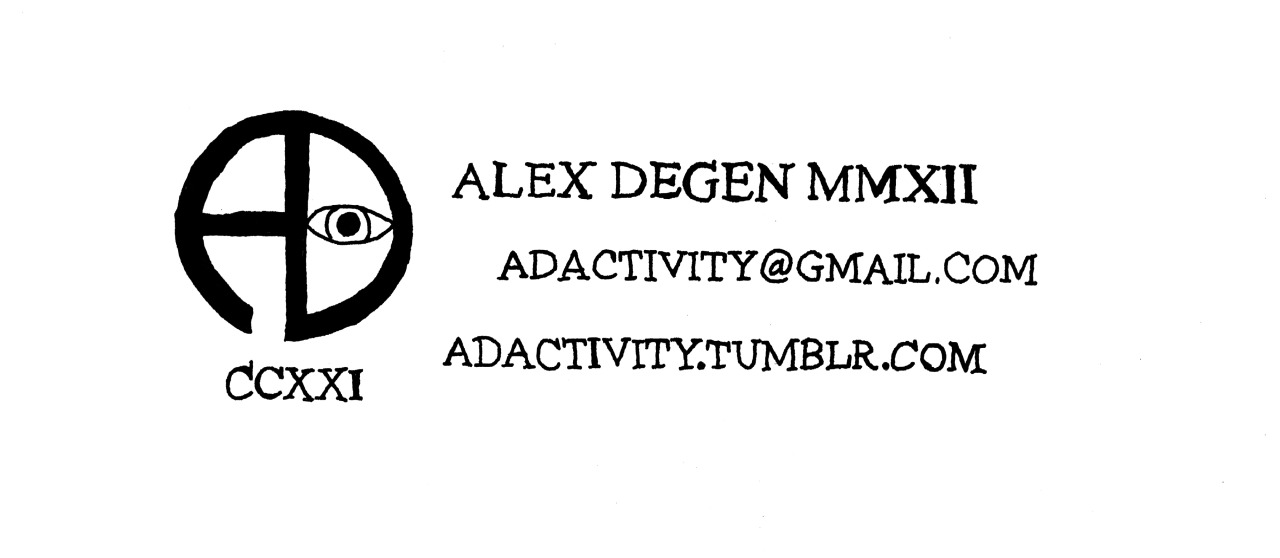
\includepdf[height=7.5in]{assets/6}

\chapter*{Past Lives}
\addcontentsline{toc}{chapter}{Past Lives}

%\includegraphics[width=5.03125in,height=7.55373in]{media/image9.png}

Cash laid on his back in the bed of his truck, staring up at the milky way above. The hill that he'd parked on was just far away from the city to null out the light radiation. He could hear the soft rustle of the tall grass swaying with each small breeze that passed through. Despite the tranquility of the scenery, his heart was racing in his chest.

Next to him, he felt the fox's tail curl in and out at his side. It lightly brushed him, but never lingered long. He thought of moving his a little more towards it, so that their tips might touch. Every time he tried though, the signals from his brain stopped just shy of letting him actually do it. The moment was right, but he couldn't bring him to move an inch.

Cash licked his lips. They felt more dry the longer he just lay there on his back saying nothing. If this was the closest he could get to admitting his feelings, that'd be fine too. He just enjoyed Wade's company and that was almost enough to satisfy him.

"You think Mr. Owen will assign us a pop quiz tomorrow morning?" The fox asked, referring to the chemistry class they shared.

Cash shrugged at first, saying, "Maybe." His head was a little too scatterbrained to focus on the question.

He listened to Wade shuffle a small amount, and he turned his head to face him. The fox had moved onto his side, gazing into his eyes. It made his muzzle turn hot and he almost wanted to turn up and face the stars again. Cash didn't though, just staring back.

Wade had a nervous smile, lifting the unique white patch of fur on his cheek. "What're you thinking about?" he asked.

A lump stuck inside the otter's throat. Everything about this seemed right, like a fairy tale romance. The crickets and wildlife on the hill surrounding them seemed to quiet, as if they too were holding their breath. Tears welled at the corners of Cash's eyes, the emotions too strong to hold back as he answered, "You."

It was the right word.

Wade reached a paw forward halfway between them as a grin formed across his muzzle. Cash took it, rolling his fingers gently around in the fox's paw pad. Both scootched forward the slightest amount, their muzzles just inches apart for only a second. Then, they folded the distance with their lips.

Cash let out a small coo inside the fox's muzzle. He grasped his paw tighter before interlacing their fingers together. Wade reached around, scooping the other teen's head gently. His claws ran through his hearfur, gently making a circle around his ear.

They remained kissing for a minute, holding onto one another. It felt like the whole universe was rippling inside him. There was a sensation like no other, and it almost became too much to bare. He had to break from the kiss, opening his eyes to see a wolf staring back at him.

\emph{Who the fuck?!?!}

Immediately, Cash's first reaction was to pull back. He tried to will his body to move, but there was nothing. All he could do was lay there frozen. His mind was racing, taking in the environment around him. This wasn't the bed of his truck anymore and he was laying in the dirt. There were trees surrounding him and the glow of camp fire illuminated the other boy.

The wolf pulled back from the kiss, asking, "Killick, why must we do this to one another?"

\emph{Killick?}

As his mind was racing, he felt his muzzle open to say, "Natar, I love you. I love you more than anything. I can't keep myself away."

Cash's thoughts were jarred, speaking words to this wolf without meaning to. Unwittingly, his gaze trailed down the wolf's body, seeing his nakedness. At the corner of his vision though, he could see his own body. It wasn't the short brown fur he was born with, but instead, a canid's bushy mix of black and silver.

His body didn't feel right at all. It didn't hurt, but it felt off. Like his muzzle was too long, his tail too light, and he felt cold air between his fingers where there would usually be the webs on his paws. No matter how he tried to move anything, he was just frozen reliving an event that wasn't his own.

The wolf's smile faltered a small amount and he said, "Like the ocean yearns to kiss the moon, we shall never be together. Our destinies are written and we must walk our paths."

Tears welled up along the sides of Cash's, now Killick's, eyes. His chest felt like it had been kicked in, and he experienced this wolf's sorrow. Killick's paw reached up and touched a small white patch of fur on the other wolf's cheek. It was similar to the distinct markings on Wade's face.

"Is it really written? The kiss of the dreamer? Do you really have to go?" Killick asked.

Natar nodded his head, holding back tears himself. With a shake of his head, he tried to ward off his sadness. "It's not so bad. It's an honor to be the vessel of a god, but this is only a dream. I must awake from it," he said, reaching a paw forward to touch Killick similarly. "But the oracle told me something amazing."

Cash listened with Killick, feeling his ears perk up. Both himself and the body he was inhabiting asked at once, "What did the oracle say?"

Natar brought back his smile to its fullest and whispered, "She said that in the dream that is now, I am destined to be with the one I love. Always and forever."

With that, the two wolves moved closer and wrapped themselves around one another. Their lips met, the warmth of their bodies mixing, and just as they were pulled into their passion, Cash ripped himself away.

Wade, startled, let out a small yip as Cash's paws pushed him back. "I'm sorry," the fox blurted quickly, starting to pull himself upright on the bed of the truck.

"What the fuck?!" Cash cried out, flipping his head back and forth. "Where's Natar?" he asked, feeling a longingness, like the love of his life had just been ripped from his paws.

The fox curled himself away, ears folded back and looking around for whatever Cash had been searching for. "Natar? I--- I don't understand?"

Cash put a paw to his chest, his heart thrumming like a drum. It took him a second to even realize where he was again. He placed his paws on the bed and lifted himself up, still breathing hard through his nostrils. Tears rolled down the sides of his muzzle, but he wiped them away quickly.

"I'm sorry," Wade apologized again, now pulling himself to his feet. "I thought that---"

"---No!" Cash said with a paw out to stop him. "No, I do--- I like you a lot."

Wade's head cocked in confusion, not understanding the situation. Cash barely understood it himself. "I'm sorry," the otter said, trying to calm himself down. "I thought I saw something."

The fox stepped to him, reaching a paw down. Cash didn't take it immediately, scared of the touch. He cautiously reached for it though, holding his breath before touching his finger's to Wade's. Nothing happened. A long sigh of relief escaped from the otter and he took his paw, helping himself up.

When they were standing in the bed of the truck together, Wade stepped forward so they were close. "You like me too?"

Cash, relaxed now, interlaced his fingers with the other teen once more. They stood together under the stars. "Yeah. I like you a lot," he said, and they bowed their muzzles and touched their foreheads together.

Wade asked, just above a whisper, "Will you be my boyfriend."

Their muzzles went up, just barely apart, as he said, "Yes."

That night, Cash drove Wade home with the fox curled against his side in the cab of the truck. He planted a kiss on his cheek before he dropped him off in front of his house. When the otter got home though, he spent the rest of his night on his computer searching for the names Killick and Natar. It was a fruitless search, and he only gave up when the dawn was peaking through the curtains of his window.

\secdiv

Weeks went by, the two only growing closer with each passing day. Cash made no mention of the vision and he gave up trying to scrounge the internet for anything that would remotely make sense of what he saw. Trying to look up past lives or anything supernatural was an even dumber pursuit. Most sites he found seemed closer to fantasy than anything factually useful.

The news of Cash and Wade being together came as a surprise to absolutely no one. Most of the comments rang out as, "Finally." shared amongst most of their friends. Even the otter's parents knew it was coming when he shared it with them. Wade's parents were cool with it too, and that was the biggest relief to him. Things were working out.

They were in their friend's basement, with the fox's head resting in Cash's lap. He rested a paw against his boyfriend's neck, scratching at it softly with his claws. Trevor, a chubby badger seated on a loveseat next to them, took a hit of his blunt, exhaling it out slowly before stating, "You two can just get a room, ya know?"

Emma, the raccoon reaching a paw out for Trevor to pass the joint, asked, "Get a room where?" The badger handed it over and she took a small hit before saying, "I think it's cute."

They all laughed at that and when Emma offered to pass the joint to Cash, he shook his head. Wade however, turned his paw out and she leaned over to give it to him. He watched as his boyfriend took it into his lips, breathing it in before letting it out slowly. The smoke rose, tickling the otter's nose until he let out a sneeze.

Wade giggled and said, "Sorry," before he turned it over to Trevor again.

When the fox turned back to Cash, he stared down into his eyes for a second. In a blink though, his amber irises shifted to emeralds. He tried to squint, thinking it might've been smoke blurring his vision. But there they were, two green eyes staring up at him. He tried to blink, but when he couldn't, he knew it was another vision. He tried to gasp but nothing happened. Again, he was trapped in another's body.

Wade was no longer Wade. Instead, seated with his head on his lap, was a beautiful snow leopard. He was the same age, a boy just like his fox. Instead of the T-shirt and jeans though, this feline was bare chested. He could see at the corner of his eye that the trousers he wore were unbuttoned.

Involuntarily, his head lifted and his friends were gone. It was an empty study, extravagant, with a fire cackling softly to the side. The room was massive, with shelves trimmed in gold lining every inch of the walls. Books were packed into them, half of the texts he knew he must've read, but he wasn't sure how.

"Jean?" the snow leopard asked, getting his attention back to him.

Cash, now seeing through Jean, paused a second and whispered, "I'm sorry. I thought I heard someone."

The snow leopard smiled and shook his head. "We checked. Your father won't be back from Amsterdam for weeks. Your mother is with her sister. It's just us."

Jean let out a sigh, reaching a paw down to stroke between his ears. "Dion, I cannot be paranoid enough. If I could, there'd be guards lining the building at every corner with bells in their paws."

That got a chuckle from both of them, though Jean was still nervous. Cash could sense that the aardvark's sentiment was true\ldots{} Aardvark? Cash could now see the fur on his arms was thin and short. His nose at the end of his snout looked vastly different and he wanted to wrinkle it. It didn't move. Instead, he just kept his attention on Dion below, focusing on the touch of his fur. There was that same white mark on the feline's muzzle that Wade and Natar shared.

Cash fought against the vision this time. He was going crazy and he just needed to tell himself he was back in Trevor's basement smoking weed. Maybe it was the contact high that was causing it, but he'd smoked with his friends dozens of times and never had this happen before. The otter focused hard, trying to get back to reality.

His vision started to crumble and he could see Wade mixing with Dion underneath him. Involuntarily though, his muzzle opened and he heard himself and Jean say, "You are the most precious gift in my life. I am humbled by you. All my riches, my status, my being is all but shades of pale gray compared to the kaleidoscope of your love. You are the blood in my heart and the breath in my lungs."

Cash watched as tears weld both in the snow leopard's and the fox's eyes. Without meaning to, his muzzle dipped down and he gave a soft peck to his lover's lips, just as Jean did to Dion. As he pulled back, the bright colored study began to break away. He turned his head to the fireplace until it disappeared, and only Trevor remained with his maw gaped.

"Dude," Trevor chuckled, and Cash shook his head, now fully out of the vision.

Emma reached her paw towards the badger, though her muzzle was also facing Cash. "Wow, that's intense," she commented.

Cash took a gasp, like it was the first time he could breathe air again. His muzzle flipped down towards Dion--- no, Wade, on his lap, but the fox didn't sense the worry. His eyes just listlessly stared up at him and he had an open-mawed smile on his face. "Where'd that come from?" he asked in a chuckle of disbelief.

Cash slowly shook his head and said, "I dunno."

The vision was still crisp in his mind, but he didn't mention it. He didn't want all of his friends to think he was losing it. Instead, he just shrugged it off and the night and went on like normal. They continued to smoke until they had to walk back home. Jean and Dion were still in the back of Cash's mind.

\secdiv

"Faggots," a tiger named Austin called out as the Cash and Wade walked between classes paw in paw.

Cash stopped, and he felt Wade's grasp squeeze between his web fingers. The fox leaned into him, whispering something, but he didn't hear it. His head spun quickly to the bigger boy, asking, "Excuse me?"

Austin was leaning against a locker, but had now pulled himself off of it to turn and face Cash. "Deaf and queer?" he started, puffing himself out a bit in a show of intimidation. "I said, Faggots."

Cash let go of Wade's paw, but the other boy still held onto it. Even when he turned to face Austin, his boyfriend still held onto him, saying louder this time. "Just ignore it."

Austin gave a mean smirk, muzzle pulling back on one side to show some fang. "Listen to your bitch and keep walking. In Fact, just keep going right off a bridge," the tiger said, getting another step towards the two.

Wade gave him another tug, trying to lead the otter away. Cash yanked his paw free and got closer to the tiger. His arms were already up, and he gave a push to Austin's chest. The tiger was forced back only a slight bit, and he could hear feet shuffling around him as other students circled to see the commotion.

"Don't fucking touch me!" Austin shouted and then swung a fist straight for the otter's muzzle.

It collided against his cheek hard, and Cash was knocked off his feet. He landed on the ground hard, panting through his mouth. The side of his face stung, but not quite like his knuckles. When he pulled himself up, he was still on his knees, but there was a kangaroo underneath him.

Cash gasped in shock, seeing the marsupial's bloodied face. It was a man, not much older than himself. He was reduced to shallow breaths, his head leaning to the side. His eyes seemed to be peering into nothing as he stared at a red brick wall in an alley.

\emph{Not again}.

"Reese!" he heard a voice call back to him.

Cash's muzzle turned behind him, though it wasn't of his own volition. Standing in the alley's entrance was a possum with his paws clasped around his muzzle. He stood frozen, and an overwhelming sense of guilt flew through Cash's mind. "Keith? What're you doing here?"

At that, the other teen rushed over. His head turned back behind him in concern, and it seemed like he was hurrying over as silently as possible. Cash, now Reese, looked down at the kangaroo and said, "He followed me into an alley. I had to defend myself."

Even Cash knew that was a lie, though only partially. He tapped into Reese's memories unwittingly, seeing himself walk into the alley knowing Jeremiah was following him. But he had led him there, and jumped him the second he could. He could still hear the kangaroo begging for him to stop echoing in his head.

Keith got to his side, pulling him up. When Cash saw his own bloody knuckles and claws, he could see they were feline. He stared at them in horror, shocked at what he was capable of. The possum pushed him to the side against a wall and hissed, "What'd you do?"

That guilt that he had remained, but Reese shrugged it off. "What needed to get done. He wasn't gonna leave us alone," he said, eyes averted away.

Keith shook his head with a deep frown on his muzzle. "I don't like this side of you. It scares me," he said, tears falling down the sides of his muzzle.

Reese tried to reach a paw up to wipe away some of his lover's tears, but Keith pulled back. He saw the blood dripping from his paws and the possum took a step back. He shook his head once, and then turned to walk away.

"Keith, please. It won't happen again," Reese begged, but that didn't stop him from leaving.

Reese let him leave, shaking his head in disappointment at himself. He pulled out a handkerchief, wiping his paws as clean as he could. There was one final glance to the kangaroo, beaten and bloodied before he turned to the entrance of the alley and started a quick jog to catch up with the possum.

As he did, Cash, still inside of Reese's head, could make out the street. There were cars along the road, but they were older vehicles. He'd recognize them in old movies from the fifties and sixties. Across the street from him was a theater, bright and polished now, but long since abandoned in his own time. This was\ldots{} his hometown, but half a century ago.

Reese caught Keith hurrying down the street and held up a paw towards him. "Keith. Wait!"

The possum stopped in the middle of a crosswalk, turning his head to face him. He stood there for a second, eyes full of sorrow. Reese started to move forward, but at the corner of his eye, he could see a car coming from the street. Cash and Reese let out a gasp, watching in horror as the driver was just inches from colliding with Keith.

"Keith!" Cash screamed out as he flung himself forward on the ground.

The entire hallways seemed to flinch at once, everyone drawing backwards. Cash lifted his head, flipping it around back and forth. It took him a second to realize where he was, or even, who he was. Reese still lingered in his mind, his memories conjoined with his own. He could see himself, a tabby cat with his partner, Keith.

He felt paws on his back, grabbing his shirt hard enough to cut tears into the fabric. "The fuck's wrong with you, freak?" Austin asked as he hoisted him back to his feet. "You want a fight? Let's g---"

Cash spun around, his arms knocking away the tiger's as he got to his feet. Instinctually, he clasped both of his fists together at once and swung at Austin's muzzle. His strike hit him hard, and he watched a fang and blood spit out of one side of his face. There was a dazed look in Austin's eyes, and he wasn't fully there anymore.

Before he could let him react, Cash's knee went up into the tiger's gut. Austin couldn't even brace himself, body folding forward as the wind was knocked out of him. The otter watched as the other teen let out a nasty sound from his throat. Then his body collapsed to the ground with a slump.

Cash, with Reese still in him, was burning with rage. This wasn't over for him yet. Without thinking, he got down on a knee over the tiger. His arm went back, fist clenched tightly. A single punch went to the side of Austin's head, and he heard his skull bounce against the tile floor underneath.

Cash drew his arm back again, ready to hit him another time, but a paw wrapped around his wrist. His head spun back in anger, and he let out a growl. Only when he noticed it was Keith--- no, Wade, holding him back, did he realize what he was doing. He stared back at the fox, slowly coming down from his rage.

A whistle blew, and Cash's ears ducked to the sharp pitch. All the students came into view, and he realized the crowd that had gathered to watch. His head began to spin, the eyes all on him too much. He pulled his paw from Wade's grasp to place it over his brow. Murmurs surrounding him mixed with the groans of the tiger beneath.

The campus security broke through the crowd, and Cash was quickly taken to the vice principal's office. He didn't see where Austin went, but he figured he was with the nurse. He'd never hit someone before in his entire life, but the way he went after the tiger was unnatural. It terrified him.

Three day suspension and detention for a month was his punishment. It couldn't have come at a worse time. Cash was at the last stretch of his senior year and it was going to be spent an hour after school in the detention ward. His parents were livid, and there was even talk about sending him to anger management therapy.

"I didn't mean to do it," Cash whispered, leaning against the seal of his bedroom window.

Wade nodded his head up and down, though it was reserved. The fox had snuck into his backyard and leaned inside of his bedroom. He'd tried to come earlier that night, but Cash's parents assured him that he was grounded and wasn't allowed to have visitors or boyfriends over until he had learned what he'd done.

Wade, nervous, said, "I've never seen you do that before." There was a small pause before he added, "It scares me."

Cash remembered Reese and Keith, that same thing the possum said to his boyfriend. The otter's lips trembled a bit and he wanted to tell him of the visions he'd been having. It felt more like an excuse though. All he'd really done was channel Reese's skills. He couldn't deny that the anger was his own, and anyways, he didn't want to worry him about something he could barely explain himself.

"It'll never happen again," Cash promised, reaching a paw across the window and grabbing hold of Wade's.

The other boy took it, but his clasp was loose. There was something on his mind. "Is everything--- I mean, outside of this, is everything alright?"

Wade's eyes turned from the otter's eyes and he gave a small nod. "Yeah, just shooken up a bit," he started. He could see the fox put effort into meeting his gaze and he said with a small chuckle, "Everyone's talking about you. I didn't know I was gonna be dating a celebrity."

Cash let out a small laugh and shook his head. "They'll forget about it before the weekend. It's not like there aren't fights that happen," he said, and then, trying to play it off, he flexed his arm and added, "Bet no one's gonna mess with us now."

Wade's eyes narrowed and he quickly pointed out, "You said it'll never happen again."

Cash quickly put his arm down and blurted, "Yes, of course. I mean, I don't even think I could do that again. I just mean---"

Before he could continue, the fox leaned forward into his bedroom and stopped him with a kiss. Cash let out a sigh through his nostrils and crooked his head to return the kiss. Their muzzles locked for a minute, both boy's tongues touching against one another. It only broke when Cash heard the sound of a creek just outside his bedroom door.

The otter's mom opened the door, and Cash was sitting, hunched over his desk. She flicked her head to the open window before turning his attention back to him. "Were you talking to someone?" she asked, though, it seemed like she knew the answer.

Cash turned his entire seat to face her, and then back down to the textbook in front of him. "No, just to myself. Helps with math," he lied.

She studied him a second longer, took a step into the room but then stopped. His mom waited there with a paw on her hip before exhaling. She turned back to the door, stepping through it and saying, loud enough, "Cash, can you make sure to close the latch to the side gate before the end of the night. It was left open last time."

A grin worked its way up the side of the otter's muzzle and when the door was closed, he got back to the window. Wade appeared with his ears ducked and a sheepish smile on his muzzle. "Oops," he mumbled, before they resumed their kiss.

\secdiv

The suspension blew by quicker than Cash would have thought. Wade brought him his homework each day to keep his grades up. He needed them to see if he was gonna get into school with the fox. As the semester was drawing to a close, the anticipation for acceptance letters grew.

Returning to school was mostly normal. Austin didn't bother him once. In fact, the tiger was quick to scurry away if Cash got anywhere near close to him. It wasn't just that though. Students in general seemed to stay a safe distance away from him when he was walking with Wade. Even his friend group seemed a little nervous to disagree with him.

Cash needed another side of these visions. He knew they weren't just his imagination or some sort of mental breakdown. They were so clear to him, and he could see them at the corners of his eyes whenever he was close to Wade. Sometimes, he could even make out the sounds of small whispers gathering just beyond ear shot.

"Cash," Wade said, trying to get the otter's attention.

Cash turned his muzzle to his boyfriend, only realizing now that he was being talked to. "Yeah?"

They'd been on the bed of his truck, legs dangling above the unfolded gate. The fox put his arm on his, and stroked him up and down. Both had been quiet all night, but Cash had just assumed that it was because they were enjoying each other's company. It was clear now though that something was on the other boy's mind.

"Did you get any acceptance letters yet?" Wade asked with some hesitation.

Cash scoffed and shook his head, "Nah, not yet. Why?"

The fox ducked his head low, brow furrowed in thought. He paused for a small while and then said, "I've been meaning to tell you."

He leaned into his boyfriend, afraid for the worst. Wade was smart, active, and unique. Any school would be so lucky to have him. Cash pulled the fox's arm to him, trying to comfort him. He didn't return the affection and said, "I got into UC Golden."

Cash's ears perked up, a smile forming on his muzzle, "Dude! You did it!" He pulled his boyfriend into a tight hug that was only met with a small grasp. He pulled back, trying to read his boyfriend's muzzle. "What's wrong?"

Wade turned his muzzle to the side and whispered, "I've\ldots{} I've known about this for about a month now."

Cash cocked his head to the side. "Why didn't you tell anyone? Why didn't you\ldots{} why didn't you tell me?"

The fox reached a paw up, rubbing at his eyes as tears began to form. "I just--- I was waiting to see--- you're sure you haven't gotten any mail?"

It was at that point that he realized why he'd not told him. A vice gripped over his heart. Cash had to shake off the dread and said, "We're both in the exact same classes and we practically get the same grades. Maybe my letter is just lost in the mail or something. I'm sure we'll both be going to UC Golden."

Wade nodded but it lacked any confidence. "Yeah, probably," he agreed, but then added, "I'm just nervous."

Cash, trying to add some optimism, said, "Look, no matter what, we'll be fine." He dipped his muzzle underneath Wade's and kissed his neck. The fox leaned against his shoulder, letting out soft murmurs. "I love you."

Wade pulled suddenly, muzzle hot with embarrassment. He didn't say anything, and Cash opened his muzzle to try and take it back. Or at least, play it off. Maybe he was rushing things too fast, but the sound of a fire cackling distracted him. He turned his muzzle back, seeing a fireplace in the middle of the hill the truck was parked on.

Then he turned his head back to Dion, the snow leopard sitting on the chaise lounge with him. He was Jean the aardvark again, and they were back in the study. The other boy had a concerned look on his muzzle. His maw split in a dismissive smile.

"You do not mean that," Dion said, shaking his head back and forth.

Cash watched himself lean in, reaching a paw out for the snow leopard. "Of course I do. I love you. I mean it more than anything."

Dion continued to shake his head, rejecting the paw out towards him. "You don't love me. You order me. This is not romance. It's a transaction. I am not your lover. I am your courtesan."

Cash felt Jean's hurt, and his paw recoiled. His head went down, and he sheepishly looked at his crotch. He thought for a second before saying, "It is only because the roles we were given that it is like this, but you cannot deny it. What we share is true. What we feel is real. And\ldots" he paused, looking up to Dion again before finishing, "our love is undeniable."

Tears welled up along the corner of the snow leopard's eyes. He reached a weary paw up, brushing away a tear with his claw. "I don't want your love. I want your money," he said, trying to make a stern face.

Jean lifted from his seat, walking towards the other boy. "Take it," he said. Dion took a small step back, but Jean closed the gap and repeated, "Take it all. I wasn't born to want it anyways. You can have every penny of my wealth if that's all you care for."

Dion turned his head to the side, like he'd be caught bluffing. Reached his paw up, clasping the snow leopard's cheek and pulled him forward. Their muzzles locked and their chests pressed against one another's. Before they could continue though, there was a sound from outside the study. Footsteps. Lots of them.

"Hide," Jean said as he broke the embrace.

Before Dion could even get a step away, the doors across from them bursted open at once, and a taller aardvark dressed in a uniform came rushing in. Jean stepped in front of the snow leopard, maw opening to speak, "Father, this wasn't---"

"Do not lie to me," the older aardvark said, charging towards him. "You've brought enough embarrassment to this house!"

Jean took a step towards his father, paws out to slow him. Lightning fast though, the older man lifted his paw up and a backhand came rushing towards his face. Cash hit the side of the truck, falling onto the bed just as Jean took the hit. The otter grabbed at his own muzzle, feeling heat as if he was just struck.

"Cash!" Wade cried out, rushing to his side as he watched him go down.

Cash flung his arms up, crying out, "Father! Don't hurt him!"

The otter flipped his head back and forth, trying to find Dion. It was nothing but the bed of the truck and the surrounding hill it was sat on. He couldn't see the fireplace nor the bookshelves anymore. Only the tall grass and the distant lights of the city could be seen.

Wade pulled back, asking, "Cash? What's going on?" His muzzle was full of concern and he looked like he was about ready to tear up.

Cash put a paw to his head, still split between his own memories and Jean's. He had to piece together where he was and\ldots as scary as it sounded, \emph{who} he was. Slowly, his own timeline began to come together, but he felt like he was seeing double.

"It's nothing," he said with a grunt. "I'm just--- I got a headache."

Wade, shaking his head and snout scrunching up, growled, "It's not nothing. You've been acting weird. The fight. These little outbursts. What're you not telling me?"

Cash scootched himself off the truck's bed, standing on the ground. "It's just a headache. It doesn't matter. I'll be fine, Dion--- Wade."

The fox caught it, brow going up, "No, see. Right there! You called me---"

Cash, waving a paw out quickly in front of him like he meant to push away the other boy, hissed, "I said it's fine!"

Wade stepped back, muzzle going down to the ground. The fox stood there silently as Cash tried to collect his thoughts. He was almost too focused on himself to see the hurt he'd caused. Only when he looked at his boyfriend clearly, did he realize what he was doing.

Wade mumbled, "I'm sorry. I\ldots I love you, too."

Cash quickly folded the distance between them, embracing his boyfriend and stroking him down his back. He could hear Wade start a small sniffle and he quickly shushed him. "Shh, no no. I'm sorry. I'm so sorry. I want to tell you, but\ldots" he thought of what to say, if he could be honest, and instead said, "I'm still figuring things out myself."

Wade was quick to calm down, but they didn't have much to exchange afterwards. They got into the cab of the truck, and he dropped off his boyfriend. All the while, he had to fight off the memories still floating in his mind. He could remember poetry lessons, horseback riding, the first time he'd purchased a night with Dion, and even a little bit of French he'd never learned before.

There were cracks of lives lived leaking into him.

When he walked into the house, the first thing he noticed was his dad on the couch. His mom was with him, and they were wrapped under a blanket snuggling one another. He couldn't take his eyes off his father and the older otter noticed it.

"Did everything go well?" his father asked, reaching for the remote to pause the TV.

There was an anger, not his own, that stuck with him. It ate at his insides. He had never been scared of his dad before, but part of him said to be terrified. Like this man he'd known all his life, a kind and gentle otter, was willing to strip away all that he loved in order to save face.

"It went well," he said a little sharper than he meant. That got his dad to cock his head towards him, and he quickly corrected himself with, "No, it went great. Thanks for asking. You two watching anything good?"

That night, he sat on the couch and watched a goofy Doug Riot film with his parents. He had to remind himself who he was, who his family was to him, and which life he was living. At the end of the movie, he kissed his parents on the cheek before going to bed, knowing now just how lucky he was to have them.

A week passed and the letters did come. Cash's parents sat at either of his sides as he unfurrowed them in front of himself. He set the one with \emph{UC Golden Admission Department} aside, saving it for last, and grabbed the one for his backup schools first. La Jolla State was the first one he opened, holding his breath.

"I got in!" he shouted with a breath of relief. His parents hugged his shoulders.

There was a mix of rejections and acceptances, but eventually it came down to the one. Part of him knew what it would be, and he took in a gulp. With the letter opener, he cut through the envelope's lip and read the letter to himself. He didn't even need to scan the entire thing.

\emph{We regret to inform you\ldots{}}

\emph{*****}

"Dude, that sucks," Trevor said, slumped into the couch. He dipped his muzzle towards the lips of the bong and took a rather big hit before blowing it up to the ceiling of the basement. "Sorry," he started before letting out a couple coughs, "you didn't get in."

Emma, a little bit more self aware, didn't reach for the bong. She sat on the floor, watching Cash with her ears splayed. "What're you gonna say to Wade?"

It was on his mind all week. School was ending, but even then, the fox had to pass on their session so that he could cram in studies. If Cash did that more often instead of smoking his buddies, he probably wouldn't even be in this situation. That guilt had been growing in him the longer he had put things off.

"I dunno," Cash said, leaning in and grabbing the bong from Trevor. He needed a hit.

The otter lit the stem with a lighter, muzzle wrapped around the lip. He took in all the smoke, pulling back and holding it in his lungs. Even as a mustelid, the smell was a bit too strong for him and it felt like his whiskers were on fire. Trained though, he leaned his head back and let it all out into the air.

The weed fuzzied his mind a bit, and without thinking, he said, "I guess we'll just break up."

He didn't notice the silence that followed after. Cash was lost in the high for a minute, just existing. Emma had to snap him out of it, waving a paw in front of him as she said, "You're gonna break up with him?"

Cash turned his muzzle to her, a little frazzled. "No? I mean, um, I'm just spitballing ideas. What am I supposed to do?" Trevor took the bong from the otter, and placed it on the coffee table in front of the couch. Cash sighed and asked, "Do you guys ever get the feeling that some things weren't meant to be?"

Emma looked at the bong and snickered, "Do you ever get the feeling you might've smoked too much?"

Cash grumbled at that, shifting uncomfortably on the couch. "I'm being serious."

Trevor shrugged his shoulders and said, "I dunno? Maybe? I guess the only thing we can do is try our best?" His words lacked confidence.

The otter thought of what he said, pulling out his phone. Emma saw it and the raccoon's muzzle scrunched up. "You're not gonna call him, are you?"

Cash's muzzle turned hot and he flicked the screen on and off quickly, "No," he said defensively. "Just checking the time."

Emma rolled her eyes and sighed. "Hey. It's gonna be alright. You got into La Jolla, and that's a good school to be in. It's not even that far away from UC Golden. Certainly much closer than University of Apple is," she said with a small pinch of disappointment.

It was that time. Emma would be going off across the country to study law soon. Trevor would probably stick around here and take some community college courses. And Wade, if he wasn't going to be an idiot about it, would be going to UC Golden. Cash felt a little bad making this night about himself.

"Hey, um, congratulations on Apple though. That's a pretty big win," Cash said, hoping to instill some optimism in the conversation.

She nodded, saying, "Thanks. I'm excited." before reaching to the table and grabbing the bong for herself. These precious moments with his friend group were fleeting and he needed to make the most of them. So, they got high, and spent the rest of their night laughing their asses off.

\secdiv

Wade was sitting on the otter's bed later that same week. Cash's parents let the fox back into the house, figuring he'd learned his lesson about the fight. The door was cracked open though, a new rule for having boyfriends over, even when it was the weekend.

Two letters sat on his desk, but he hadn't brought them up all night as they watched videos on his laptop screen. He was meaning to talk to Wade about it, but every time he wanted to say something, his mouth felt dry.

"You want another soda?" Cash asked, getting up off his desk chair.

The fox reached over to the nightstand, wiggling his can before saying, "Nah, it's still mostly full."

Cash nodded and walked out of the room. He made his way down the stairs, turning into the kitchen to grab another soda. Curiously though, he peaked his muzzle into the living room to \emph{see what movie his parents were watching} and noticed that the TV was off. Checking the couch, he saw it was empty.

Quietly, Cash walked around the house, just so happening to find his parent's room. He tiptoed to the door, looking at the floor to see if any lights were on. Just like the rest of his home, it was dark. The otter pressed one sharp ear against the door, holding his breath. Softly but surely, there was the sound of two distinct snores.

His heart was racing as he got back to his room, forgetting the soda he meant to grab. Wade was still on the bed, sprawled out on it and looking a little tired eyed. Cash was anything but tired at that moment. He closed the door behind him, and turned the lock.

Wade heard the click, eyes going up to the otter curiously. "I'm probably gonna have to go home soon," he said quietly.

A smile flicked across Cash's muzzle as he whispered, "My parents are asleep."

The fox didn't seem to immediately get it. "I guess I really should go home then."

Cash's brow furrowed and he shook his head. "No, um, maybe you stay the night?"

At that, the two triangles atop of Wade's head danced upward. A soft glow of pink spread across his muzzle and he whispered back, "I dunno if my parents or your parents would like that."

Hormones answered for Cash. "Who cares what they think. I just\ldots I want it to be us tonight."

Wade got to a sitting position with his legs dangling over the bed. Cash took a spot next to him. They sat there for a second, paws on their lap. Every passing moment felt like hours, and it was a full possibility if neither moved, they'd just stay like that until morning came. But Cash took a shaking breath in, and slowly moved his paw onto Wade's.

And that night, it \emph{was} just them.

Cash woke up next morning, slightly startled when he felt the warmth of fur at his front. He pulled back, waking up Wade in the process. The fox took a sharp breath in, rolling over and looking at him curiously. Their muzzles grew hot and Cash dipped his muzzle sheepishly.

"Um, good morning," he said with a small chuckle.

Wade leaned in and gave him a kiss on his cheek. Cash returned it. "Good morning," the fox said back listlessly.

There was a stickiness on the otter's fur, reminding him what they had done and the only thing Cash could think of to say was, "Last night. I--- I hope you enjoyed it."

They didn't exchange much more than love yous before passing out the night prior. Now, they were sitting in an awkwardness Cash had never shared with anyone before. Wade seemed content though, and he said back, "I did. I love you."

They kissed once more before Cash got up off the bed. He placed an ear to the door, and could hear his parents up and walking about. His heart sank and he turned back to Wade, looking like he might pass out again. "My mom and dad are up," he said.

Wade looked to fully awaken at that, a small nervous smile spreading along his muzzle. "Should I go out the window?"

Cash rubbed at his wrist at first, feeling like a bad boyfriend at first. Then his eyes lit up with an idea and he gave him a grin. "Yeah, but then just come around to the front door and pretend that you just got here. I'll see if dad can make us breakfast."

A devilish grin was shared between the two boys. Wade got off the bed, finding his clothes scattered across the floor. Cash went to his drawers, grabbing his weekend PJs and putting them on as well as a loose fitting shirt. He was about ready to go to his door, turning back to see the fox with a leg out the window.

But that's when he noticed it. Wade was frozen, head and body still inside the room. His eyes were pointed downward to the desk. Cash followed his gaze straight down to the admission letters he'd left out. He was staring at them with his maw open.

Wade's eyes turned to face Cash, and he sputtered, "I was---"

"Cash? Are those?" He stopped speaking and got back inside the room.

The otter walked to him, whispering, "We can talk about it later. I promise."

Wade shook his head, grabbing the letters off the desk and pulling them up to his muzzle. Cash tried to snatch them out of his paw while still trying to be silent. He could see the other teen's eyes darting across the page before they stopped. Then he looked up at the otter.

His bottom lip trembled. "You\ldots{} you knew?"

Cash averted his to the side. "I was going to tell you, but\ldots I just---"

The fox squinted his eyes closed, brow furrowing like a headache was forming. He practically threw the letters behind him and then pushed past Cash. He walked straight to the door, opening it before slamming it behind him. Cash spun around pleading, "Wait!"

He grabbed the handle and swung the door open, only it wasn't his hallway in front of him. Instead, there was a crowd of wolves, their backs all facing him. It wasn't morning anymore. It wasn't even a house. Instead, it was outside in the deep of night with torches illuminating the scene.

Killick stepped forward, and Cash was moving with him. The wolf reached his paw forward, pushing past two of the wolves. He muttered apologies as he fought his way through the crowd. There was an intense feeling of grief and regret in Killick's chest, and it overlapped with Cash's own thoughts.

The crowd seemed to thicken, less eager to part for the wolf right up until he could no longer pass. Above, Natar stood on a raised platform to be seen by everyone. Right behind him was a long stone slab. To the wolf's right was their chieftain and to his left was the oracle. The wolfess's gaze wandered along the crowd, stopping on Killick briefly.

When their eyes met, her lips formed a small frown, but she didn't hold it. Instead, she pretended not to notice him and then continued to look out towards the crowd. A sense of being cheated overwhelmed him and he tried to move ahead again. Even when he managed to get to the front, a large wolf stood facing him. His arms were folded and he peered down at Killick with a sense of authority.

"Let me through," he ordered, and Cash felt that same anger that he shared with Reese, but he didn't know how to share his skills.

The wolf shook his head. "Killick. You cannot stop from awakening the dreamer."

Killick looked up, and saw Natar had peered down at him. The other wolf teen gave him a shake of the head, telling him to stand down. There were tears forming on his face, but he worked up a smile for him. He mouthed to Killick, "Always and forever."

Their chieftain stepped forward, arms out as he called to the crowd, "Tonight, we send our beloved dreamer back to her place amongst the gods. Natar has agreed to relinquish his vessel so that she may wake up once more and we will be blessed by our offering."

It was met with an applause that Killick couldn't share.

The oracle reached inside her gown, pulling out a blade. She turned and faced Natar, who took it with a bow. Killick stepped forward, but a paw landed on his chest. He looked up at the guard's face, but the other wolf seemed stern as he said, "He wants this. Don't make me restrain you."

Killick looked back up to Natar, who had turned and faced their chieftain. The larger wolf took the blade, and when he leaned down to accept it, he kissed the teen's cheek. Then Natar sat himself on the slab, laying down across it. That was the last time he would see his face.

Killick pushed again, and this time the guard wrapped his arms around his shoulders. He embraced him, keeping him still while the chieftain turned from the crowd. At that point, Cash, Killick, Reese, Jean, and a hundred other voices were all screaming at once. They fought hard, but they couldn't do anything as the blade went up.

And then came down.

"No!" Cash screamed as he slammed his muzzle and body into the hallway across from his bedroom.

In a wild fit of rage, he began clawing at the wall, trying to break through it. He pounded fists against it with hollow thuds. Cash was reduced to tears, and folded in on himself. The otter lay in a fetal position on the floor of his hallway.

"Cash!" he heard the voice of his dad call him.

In seconds, the older otter was over him, arm slung over his shoulder. Cash quickly moved up, embracing his dad in a tight hug. He bawled into his shirt, tears soaking into the fabric of his shirt. His father stroked his back soothingly, whispering shushes in his ear.

"What's going on? What's wrong?" his father asked when Cash had run out of tears to give.

Cash pulled back, looking into his father's eyes earnestly and said, "I think I lost him."

"Wade? We saw him storming out? Did he spend the night here?" his father asked him, and though the questions came fast, he didn't seem angry or upset.

Cash turned his gaze away, still experiencing all of his past lives at once. They fought over his memories, all trying to answer at once. With wet snort, he grabbed hold of his own self, gripping it tightly until he could answer, "I did something bad."

Cash was led to the dining table, and he explained what happened to both his mom and dad. He didn't even exempt what they'd done the night prior. They weren't very happy with that, but his parents reserved judgment to the end. When he finished, they brought him into a hug and that was more than he could have ever asked for.

For the first few days back at school, Wade avoided him. He didn't show up to their group at lunch or after school. The classes they shared, he didn't talk to him and didn't even look his way. It was awkward. Almost enough to overshadow the even more awkward conversation he had with his parents about safe sex and some scolding over his actions. That weekend, he learned how to replace wallpaper.

With only two weeks left to school, Cash finally was able to reach Wade. It was at the end of classes, and with no more after school detention left, he was able to catch the fox after the final bell rang. He had to race across campus, but he managed to get to him before he could start walking home.

"Wade! Please!" Cash cried out, finding him just as he was leaving the campus.

There were students around, but he called loud enough to break through the voices. Wade stopped for a second. Then he continued along the sidewalk. That brief moment though was enough for Cash to catch up and get to his side. He reached a paw up, grabbing the fox's shoulder and giving him a small tug.

Wade spun around, flicking an arm up to brush Cash off of him. "Don't touch me," he hissed.

Cash pulled back, startled by the words. They'd been best friends for so long now, it hit hard that he could speak to him like that. There was genuine hurt in both of their faces, and the fox paused to look down at the ground. Cash was hesitant to speak, but he needed to say something.

"Please, Wade. I didn't mean to hurt you," he said. "I miss you so much."

Wade's head pulled back, like he was trying to keep in tears. "Yeah, well, you did. I didn't realize I was just gonna be some quick fuck for you before you left."

There were enough students around to gain some eyes on them. Ears were pointed in their direction, even when their muzzles weren't directly facing them. Cash looked around awkwardly, before getting closer to Wade and saying, "Can we talk? Like, somewhere else?"

Wade rolled his eyes, and tracks of tears fell at either side of his muzzle. He seemed to notice the unwanted attention too, and gave a single nod. They didn't hold hands on the way to Cash's truck. With the way they were walking, it wouldn't even be apparent they were going to the same place.

The ride up the hill was silent, and even when they were sitting on the bed of the truck, they were still quiet. Cash was hoping the fox would be the first to speak, but when it didn't look like it was going to happen, he said, "That wasn't what I meant for you to think."

Wade bit his lip and a small glare was sent his direction. "You knew we weren't going to uni together and you didn't tell me. How does that look to you?"

Cash dipped his muzzle in shame. Seeing the optics more clearly, he said, "I didn't mean--- I wanted to tell you, but it was so hard. I'm not even sure I want to go to La Jolla."

Wade rolled his eyes at that. "Of course you're gonna go to La Jolla, like I'm going to go to UC Golden. We'd be fucking stupid not to," he said, finishing that last part with a sob that built in his throat.

Cash leaned his head back, but the tears came rushing out the sides of his eyes anyways. He took in a few sniffles, thought of his words, and then said, slowly, "That's not everything."

Wade cocked his head to the side as he stared at Cash in silence. The otter brushed the back of his paw against his nose, and then wiped an eye with a palm. "I think. I've been seeing things."

"Things?" Wade asked in a whisper.

The fox just listened as Cash explained Killick and Natar, Jean and Dion, Reese and Keith to him. He went over every detail, the settings and the different situations. His paw reached over to Wade's to hold it, trying to find comfort. The two's grips were tight when the otter finished telling him about what he saw.

"You think you're seeing our past lives?" Wade asked at the end.

Cash nodded and then shook his head. "Yeah, or I dunno, something. Whenever we're close, it happens and I see them and their memories. I don't think I'm going crazy. It's just way too real to all be in my head. I'm sorry for not telling you everything."

Wade stroked along Cash's arm. "It's okay. I knew something was wrong, but I don't think I would have known what to say if I was going through that."

It felt like a relief that Wade believed him, but it was a small weight off his chest. "There's one more thing. In all the visions," he paused to let out a sigh. "They never end up\ldots we never end up together."

Wade withdrew his paw for a brief second. "Are you seeing anything now?"

"No, but, I always feel it," Cash said, keeping his voice low as if he were hiding his words from himself.

Wade fell into the otter, wrapping his arms around him. He sobbed into his shoulder, saying, "I don't want to believe it. I've never felt so strongly for another person. It killed me inside not to see you, but I can't anymore."

Cash stroked his back and said, "I think this is it. We're gonna be so far apart, and I don't think it'll be fair for either of us to try and fight it. It won't be so bad. There'll be tons of other people."

He didn't really believe that last part. Actually, he didn't really want to believe any of it.

Wade pulled back, looking into Cash's eyes and said, "If this is it, then I want to make the most of it."

Cash wiped away some more tears and furrowed his brow. "You want to keep this going? Even after what I did? Even if you know it's going to end?"

Wade reached down, grabbing the otter's palms and pulled them up. He interlaced their fingers together and asked, "Will you be my boyfriend, even if it's just for a little bit?"

Cash licked his lips. This felt like it was prolonging the inevitable. They'd only have the rest of their senior year and some of summer before they'd leave. Even knowing that, he nodded his head once and said, "I'll be your boyfriend, even if it's just for a little bit."

They kissed and in the blink of an eye, he was standing at the bus station with Wade. The months didn't seem to last nearly as long as he wanted them to. It felt like they had just thrown their caps in the air and walked straight through time. Emma was already off to Apple. They spent one last night getting high in Trevor's basement, and now they were at the end. There were no more visions in-between.

"I can't believe this is it," Wade said, backpack over his shoulder.

Cash nodded. Wade was leaving first. His parents said goodbye to him at his house and Cash agreed to be the one to take him to the station to give them time alone. They watched as all his luggage was being packed into the bus. He'd be on it for almost a full day before he would arrive in Golden. Cash would be taking his own trip not too long after.

"I'm gonna miss you," Cash said, trying not to choke up. They spent the night prior saying goodbyes, but it never felt like enough.

Wade hugged Cash tightly as he heard the call for the bus to be boarded. "I'm going to miss you too," he said into his fur.

Then he turned to the line, noticing it was already moving pretty fast. They let go, paws holding onto each other for as long as they could before they had to separate. Wade got to the back, giving one final wave as he left out a door. Cash waved back and then watched him go.

With his head low, he walked out the station. As he got outside, he turned to see the bus that Wade was on. It was just pulling out. He stopped and watched it go down the road. Tears built up along the corners of his eyes, but he wiped them away, not wanting to cry anymore than he already had.

He took a step towards his truck before he heard the screech of brakes. Cash turned towards the bus, his heart stopping for a second. There was a small fear something bad had happened, like with the rest of the visions. The bus was stopped along the side of the road and he watched the doors open.

Wade stepped out. He turned back and forth a couple times before he saw the otter standing in the parking lot. Then the fox started running towards him.

At that moment, Cash couldn't see Wade anymore. He saw Emilia and Tony, a tiger and a wolf cub chasing each other in a field. He saw Parker get down on one knee in the middle of a restaurant to propose to Andrew. Cash watched through Danielle's eyes at the top of a ferris wheel, sharing her first kiss with Eve.

Cash stood in awe on an orbital platform just outside of Jupiter. Though millions across the galaxy and solar system were there to see the event, Jianyu managed to find a place where it could be just him and Avi. They were inches apart on a bench, staring through the large glass panes in front of them.

Jupiter's bands had made up most of the view in front of them. There were screens above, showing a close up on Metis. The moon's orbit was decaying so rapidly, they could see the trail of hydrogen it was dragging across the gas giant's face. Metis's body began to rotate under the sheer strength of the planet's gravitational pull, mantle ripping apart in a fiery blaze.

A smile was fixed on Avi's muzzle as the cacomistle crawled his fingers to the other boy's paw. The mouse turned his head, at first looking down at the touch. Then he looked up into Jianyu's eyes. Just as Metis spiraled into the gas giant's body, did they close the distance between them. Their lips met right when the two orbital bodies collided.

Cash nearly missed it as Wade reached out with both paws. The otter caught him, embracing him as Wade cried into his shoulder. "I don't want to do it. I can't leave---"

Cash shushed him, holding him close. "It's fine. It's fine. You don't have to go. I won't leave you either."

The two stood in the middle of the parking lot, rocking back and forth. Cash tuned out the hundreds of thousands of lives, both past and future, humming in the background. Wade was the only life that was important to him right now. The beep of a car got them to pull apart quickly, and they gave apologetic smiles as they got out of the way.

"My parents are gonna be pissed," Wade said in a mix of a sob and a laugh.

Cash squeezed the fox's paw and nodded his head. "Yeah, I think Mom and Dad are gonna be upset too," he said, but then gave a shrug. "We'll figure things out."

Wade ducked his muzzle in embarrassment as he added, "And all my stuff is still on the bus."

Cash looked up to his truck, an added step in his walk as he pulled Wade along. "Then we better be quick. We'll catch up to them and pick it up at the first stop."

When they hopped in the truck, Wade scootched over to the otter's side. He curled against him, and Cash turned on the engine. They were off on the road when the other teen asked, "Do--- Do you think this will work?"

He didn't need to admit how far into his future lives he saw to know the answer. Cash just wrapped an arm around the fox and pulled him in close. With his eyes on the road ahead, he dipped his muzzle in and kissed the top of Wade's head before whispering, "Always and forever."

\cleartoverso
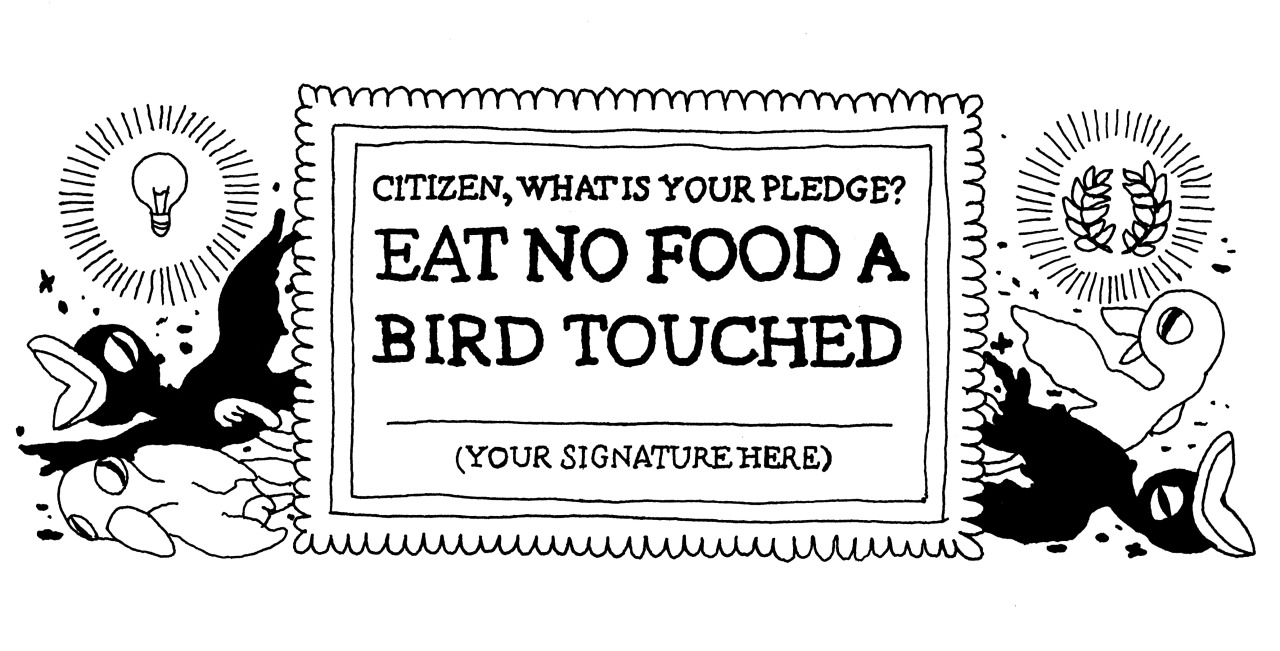
\includepdf[height=7.5in]{assets/5}

\chapter*{Taco Tuesday}
\addcontentsline{toc}{chapter}{Taco Tuesday}

%\includegraphics[width=5.03in,height=7.5399in]{media/image4.png}

Mitch grumbled to himself outside of Juanita's Bar and Grill. When his coworker, Desmond, had asked him to go out for Taco Tuesday, he'd thought it was a date. He had crushed on the wolf for so long, he didn't realize that his invitation was a part of a work outing. The raccoon didn't really want to be tagging along with the rest of the office.

Moreso though, he didn't know that the wolf already had someone with him.

Wrapped around Desond's arm was a platinum fox, chatting away giddily with all of his coworkers.

"Yeah, I go up around 7pm," he heard Richie say to a mink standing with the group.

Mitch kept an uncomfortable awkward foot away from the circle. He did his best not to look like a sour raisin, but it strained his muscles trying to fake a smile in front of everyone. His eyes kept moving to the vulpine, and a pang of jealousy would overcome him every time. Richie was beautiful, charmy, funny, and apparently a talented musician as well. He had everything going for him.

"That's so cool," the mink, Andrea, said, leaning into the couple. "How long have you two been seeing each other?"

Desmond's ears turned a slight shade of pink, and he bashfully turned to the fox. "Oh, I dunno. Almost a month now, right?"

The raccoon's ears flicked to the conversation, a small hope that this wasn't anything serious. Richie snuffed that thought out as he leaned in and gave a peck to the wolf's cheek. "It feels like longer. We've been hanging out almost every night. He's very supportive."

They shared a giggle and the wolf returned the kiss before saying, "It's hard not to be. You're very good. I just like getting into the venues for free."

The group laughed at that and Mitch rolled his eyes. Never once did the wolf seem interested that he could play music. He was actually pretty good at playing the guitar himself. Mitch could play any of the silly love songs that he would want to hear. In truth, he wanted to play them all for him.

\emph{B}zzzz

Mitch looked down at the humming pager in his paw. "Um, I think our table is ready," he said to the group.

Everyone cheered, "Taco Tuesday!" and began folding into the restaurant. Mitch was last to walk in, bringing the pager back to the stewardess. "Mitch, party of seven?" she asked and he gave an affirmative nod.

They were led to a table, the raccoon taking a seat first. Around them were pictures of desert landscapes and sombreros hanging off of the walls. Ribbons of green, white, and red were strung around the ceiling. All the staff were wearing ridiculous looking ponchos that bordered on offensive. There was even a flag in the center of each table, in case anyone forgot what cuisine this was.

And just his luck, Desmond and Richie had picked the spot directly across from him. Beside Mitch sat his other coworker, Josh, a hefty ringtail. He was the loudest in the office, and of course he'd be sitting closest to him. This night couldn't get any worse.

A twinkish hare approached the table with a tablet in hand, "What can I get started for you?"

"How bout a round of shots for everyone?" the ringtail bursted out.

It made Mitch's ears duck, and he gave a small scowl his direction. Before he could say anything, Andrea laughed and said first, "It's a weeknight. I'm not doing shots when I got cubs to go home to. Just a water for me, please."

Richie raised his paw and said, "Same. I'm going to be performing and I don't wanna be sloppy on-stage."

The hare looked at Mitch with a small smile, "Shots for you?"

Flustered, the raccoon grabbed the small drink menu from the center of the table and looked it over. Not wanting to hold up the group, he pointed to the top and said, "Just a Mai Tai for me. Thanks."

Only Desmond had taken up the offer of shots, but Josh just laughed it off. "More for us, amiright?" Then he ribbed at Mitch's side.

He inched his seat away from the bigger man, annoyed that he was in this situation. The table turned to light conversations with Mitch mostly leaving himself out of it. When he was asked for his input on something, the raccoon just gave small answers. His attention was mostly watching the fox and wolf playful nudge and hold each other across from him.

"And your Mai Tai," the hare said, smile wide.

"Oh, ugh, sure," Mitch said dismissively as he accepted his drink.

Before the hare left, he leaned in and said, "I made sure this one was made extra special for you." Then he spun around quickly, a small giggle following him.

Andrea, holding her glass to her lips, repeated with a smile, "Extra special, aye?"

Mitch, having hardly registered it, waved off her words and said, "Someone wants a tip."

Her eyebrows went up, and she took a sip before asking, "So what sort of music do you play?"

Mitch was about to open his muzzle, before he saw her gaze turn to Richie. \emph{Oh right.} The platinum fox leaned against his boyfriend for support and said, "Oh, just some solo stuff. I play the guitar and sing. Mostly covers but people seem to like them." He began to list off a bunch of pop songs, Mitch knowing how to play all of them.

Josh leaned forward after taking a shot. "Oh, that one's my favorite," he exclaimed loudly. They weren't that special, Mitch thought to himself.

On the topic of things that weren't special, the raccoon took a sip of his Mai Tai and let out a small sigh. Josh noticed and turned to face him. "What's wrong buddy? Not what you wanted?" he asked, and then gave a pat on his back.

This whole night was not what he wanted, to be honest. Specifically though, he didn't want this Mai Tai. There was a cross fox sitting at a table across from him with a salt rimmed margarita that looked absolutely delicious. He finished his drink anyways before getting out of his seat, mostly to escape the ringtail. "I'm just gonna use the restroom," he excused himself and walked towards the bathrooms.

He practically burst open the door, walking straight towards the sinks. Mitch turned the handles of the faucet, letting water spray loudly. Looking behind him, he made sure all the stalls were empty before stomping his foot on the ground. With his head in the sink, he yelled into the water, letting all of his frustrations out in a scream. Then he splashed the water into his face, hoping that it would cool him off a bit.

He grabbed a handful of towels from a dispenser. That's when he heard noises coming from a door opposite of the one he came through. Curiously, he stepped towards it, ears perked. It sounded like another restaurant was attached to the Jaunitas, but he was sure that there wasn't. It was a single building surrounded by nothing but a parking lot.

Cautiously, he reached towards the doorknob, grabbing hold of it and giving it a twist. It was unlocked, giving way at the slightest amount of pressure. His head turned back to the door he came from, only noticing now that it wasn't there. It was just a tiled wall, and he thought for a second he must've got turned around in his frustration. No, that wasn't true. This door hadn't been here before and the one he came from was completely gone.

Mitch pushed forward anyways, stepping into the restaurant. It was similar to the Juanita's, though, none of the Mexican flags and tacky decorations were no longer on the wall. Instead, they were now replaced with different sports gear and team colored shirts and flags. He recognized the orange and black of the High Kick's football logo.

"The fuck?" the raccoon whispered to himself as he walked around confused.

A guest pushed past him, forcing him out into the open as they raced for the bathroom door. That's when he saw his table, with Richie raising a paw towards him. The fox was still sitting next to Desmond. Still confused about the setting, he got back to his table and asked, "Did they change Juanitas when I got up?"

Josh gave a weird look to Mitch and then laughed loudly, "Juanita's? Jeez, those books must've been hectic today." Then, like the ringtail would, he jabbed at him with an elbow and said, "Bro, it's Wing Wednesday. We're at Hot Stuff."

Mitch recognized the name, the national brand of a sports bar and grill. Desmond, leaning forward, pointed at the margarita in front of him. "Maybe you should take a sip. Work's got you all mixed up," he said, getting a small concerned laugh from the table.

"I didn't order--- we were just at---" he cut himself off, looking at the salted rim of the margarita glass. The wheels in his head began to turn, and he reached forward to grab the stem. Carefully, he put the glass to his lip and took a sip of his drink. It was as delicious as he hoped it would be.

He put the drink on the table, looking around at the group. Everyone had eyes on him, mostly confused at the raccoon's own bewilderment. Then, with a chuckle, Mitch said, "Wow, the waiter wasn't kidding. He did make it special." That seemed to ease the tension.

Andrea, putting her elbows on the table, gave him a wink and said, "I think he likes you."

Mitch nodded his head dismissively saying, "Yeah, yeah. Anyways, when do you go up?" His attention turned towards Richie.

The fox's eyes lit up, and he could practically hear his bushy tail wagging behind him. "In, like, a little bit. I'll probably have to start getting ready in thirty."

Mitch turned his head, looking all about him at the restaurant. Most things were the same: the waiting staff, his coworkers, the cross fox sitting at the other table, and the stage ready for Richie to play in front of. But it was definitely a Hot Stuff restaurant with all the sports regalia on the walls. The staff was now wearing colored jerseys instead of the ponchos. Josh remained the same, rubbing into the raccoon again.

"Hey, don't you play? I think you mentioned that before?" he asked, strumming at an invisible guitar.

Mitch nodded his head, making a similar gesture. "Yeah, I'm alright. I know a few songs," he said modestly, still a little jarred at the change of scenery.

Josh laughed, continuing to wave his arms about like a fool. "I bet you're not as good as this guy. Maybe you should have him teach you a few things," he said, pointing over to the fox. Richie ducked his head sheepishly, and Mitch gave a frown towards the ringtail.

"Yeah, hey, I think I need to use the restroom again," he said, getting out of his seat. "I'll be right back."

Josh said something , getting another laugh from the group, but Mitch was already halfway to the bathrooms. He did not like Josh and he definitely didn't want him to be at this outing with him anymore. Mitch thought about the margarita, how much he wanted it when he left for the restroom. With the ringtail on his mind, he stepped through the bathroom door.

Everything looked the same, at least, what he imagined looked like the first time he walked in. The tiles on the wall were gray, the stalls, three of them, were black, and there were two sinks in a granite countertop. There was no door across from him. At first, he thought just to go back to \emph{Wing Wednesday} and play it out, but his curiosity led him to the sink once more and he turned on the water.

He dipped his head in, thinking to yell again but chose differently. Just brought his paws up, scooped water into them, and ran it over his muzzle. He let it cool him, grabbed some paper towels from the dispenser, and wiped his fur dry. Then, with a smile, he turned towards the door he came from, only to see it was now a tiled wall. Mitch looked over to the otherside, noticing the sounds of a restaurant coming from his right.

He walked to the new door, grabbing hold of the handle and pausing. Would it be \emph{Thai Thursday}? That didn't make much sense. Mitch tried thinking of all the things that he might have been walking into, wondering what game he was playing wandering through dimensions. Taking a deep breath, he remained stumped, but pushed open the door anyways.

Instantly, he was met with an accordion playing on the speakers overhead. There were Italian flags everywhere, along with pictures of Venice's iconic canals. The raccoon stepped out of the way of a waiter carrying a pizza tray. He looked confused at it, then turned his attention to the table. There, Richie raised his paw, waving him over.

Mitch took his seat, noticing an absent ringtail beside him. He looked over to Andrea and asked, "Where's Josh?" even though he was sure of the answer.

The mustelid cocked her head to the side in confusion and asked, "Josh? Ugh, I guess he's at home getting smashed, I assume? Were you expecting him?"

Mitch looked down at his margarita, nodding his head before giving a quick shake, "No, I guess I just thought he would've wanted to come out tonight," he said, trying to play it off. Then he asked, "So it's pizza Thursday?"

Desmond and Richie gave a look to one another and laughed, before the fox said, "I think you all called it Thin Crust Thursday? Little bit of a stretch, don't you think?"

Mitch snapped his fingers and nodded along. "Yeah! That's right. \emph{Thin Crust Thursday}," he said, as if he was supposed to know that all along.

Desmond, with some concern, raised an eyebrow and asked, "Everything good? You've been a little off all night?"

The raccoon gave a wide smile, feeling some control over his situation now. "Never better," he said, bringing his margarita to his lips. He took a long sip of it, almost tipping the entire glass back before sitting it on the table. Richie, across from him, noticed and then he began to wipe at his whiskers politely.

Mitch raised an eyebrow at the motion, before he gasped, now feeling the salt hanging from his own whiskers. He grabbed a napkin and brushed his muzzle clean before giving a silent thanks. The fox nodded and then turned towards his boyfriend, giving him a kiss on the cheek. Desmond blushed, but returned a similar peck.

Mitch didn't like that.

"You know, this margarita is really going through me. I gotta dip into the bathroom again," he said.

Andrea furrowed her brow and asked, "Are you sure everything's alright? You don't have to stay. It's just a little get together. We'll see you at work tomorrow."

Mitch held out a paw, nodding up and down, "No, it's fine. Trust me. Everything will be alright," he said, trying to hold back his devilish smile.

Then he got from his seat and walked towards the restroom. In his mind, he kept repeating what he wanted. \emph{Desmond and Richie aren't together. Desmond and Richie aren't together. Desmond and Richie aren't together}. He was so focused on the phrase that he almost ran right into the hare waiter.

"Whoops, sorry," the waiter excused himself as he took a step to the side.

Mitch looked bashful for a second, dipping his muzzle down. "No, sorry. That was my fault," he said, trying to walk around him.

The hare held up his paw, slowing him down. "Oh, um, hey. I recognize you. I think we go to the same bars?"

Mitch nodded his head before shaking it. "Yeah, um, maybe. I usually go to The Lark," he said, eyes not leaving the door to the restroom.

"Yeah, that's the one. I was wondering---"

"---Yeah, yeah. Anyways, got to go. I'll see you around," Mitch said, walking past him. He didn't even care to register the hurt on the lapine's muzzle. If tonight went well, he'd never need to go to The Lark again.

Again, he walked into the bathroom, but didn't even need to go to the sink this time. Already, a door waited directly across from him. He turned his head back to the door he just stepped through, but to no surprise, there was nothing behind him. Ignoring that, he just walked to the other side of the restroom and stepped through.

Admittingly, he was excited for \emph{Fried Chicken Friday,} but that wasn't the case. Before him, the restaurant was covered in pictures of boats surrounding him. There was a plastic Marlin hanging against a wall with nets and wooden ship wheels littering the place. Grumbling, Mitch muttered to himself, "\emph{Fish and Chips Friday}. Of--- fucking--- course."

To his surprise, Richie was still seated next to Desmond. He cocked his eyebrow in confusion before the fox noticed him and flipped up a paw for him. Mitch cautiously waved back and then walked over to take his seat. "Hey, did I miss anything?" he asked curiously.

Richie shook his head, still wearing that same smile that he had on all night. "No, you were only gone a second," he said gleefully.

Mitch, leaning into the table, asked, "So, how did you and Desmond meet?" His words were slow, cautious not to reveal anything.

Desmond and Richie turned their heads to one another, a little confused. The wolf was the one to answer. "Um, we've just been hanging out for a little bit now. I saw him play at a bar and we've just been chatting here and there."

Mitch nodded and then carefully asked, "Are you twoooooooo\ldots?" He let that last part hang until the fox's ears went up.

"Oh, haha, no. We're just friends," Richie interrupted, ears folding back.

The two shared a blush, but Mitch didn't even give them a chance to feel embarrassed, "Oh good. Haha, was just curious is all."

Desmond's muzzle twisted at that, something on his mind about the word \emph{good} in his sentence. Before he could let him speak, Mitch said quickly, "So, Desmond, you like music. You know I can play a little bit myself." He motioned playing a guitar for him.

Desmond's head went up and down in a slow nod. "Oh yeah? That's cool. Maybe you and Richie could play together sometime?" he asked, but didn't seem to be very interested in that.

Mitch, leaning in with a smile, asked, "Maybe? Or maybe I can play something for you sometime?"

Desmond nodded again, but turned his attention to the fox. "So yeah! Um, Richie, you have to go up soon, right?"

The fox let out a gasp and pulled out his phone. He glanced at the time, before nodding up and down. "That's right! Almost got caught up. Thanks," he said, getting out of his seat. "Wish me luck!"

Desmond and Richie shared a smile, one that seemed just a little too genuine. It made the raccoon's muzzle twist and he followed Richie with a glare as he walked away. Thankfully, no one noticed it.

Andrea, with a wry smile, asked, "So, this Richie fella." Her nose was pointed to Desmond.

The wolf turned to her before sinking a little into his seat. "He's great, right?" Desmond asked redundantly, but he knew what she was getting at.

She let out a giggle and said, "I think he likes you."

The wolf shook his head, but couldn't wipe away the embarrassed smile on his muzzle. "Nah, we're just friends. I dunno if he wants anything like that."

Desmond's head turned back towards the stage, ears folded back. Mitch could tell he was looking for the fox, but he tried to catch his attention. "Um, say, Desmond. Maybe you can come over to my place sometime. We could hang out. I can show you some of my guitars or we could watch a movie or something," he said, trying his best not to sound like he was pleading.

The wolf turned his head only slightly towards Mitch, giving a half nod and muttering, "Yeah, sure. We should do that sometime."

Despite it being an affirmative answer, nothing about it made Mitch feel good. It was that damn fox ruining everything. He knew what he'd have to do. Getting up again, he got a single step towards the bathroom before Andrea interrupted him. "Again? What're you doing bumps of coke in there?"

His head snapped back and he almost growled out, "No, I'm just---" He caught himself, noticing everyone at the table was now staring at him. Breathing in, he let out a long sigh before saying, "I'm just fixing something. Don't worry about it. I'll be right back."

There were murmurs shared between his coworkers, but Mitch just ignored them. They couldn't understand how important it was that he got this right. Richie was ruining everything that he wanted, and all he needed to do was remove him from Desmond.

That fox gotta go.

Mitch wanted nothing more than for Desmond to have never met Richie. He grabbed hold of the bathroom door, thinking about his wish carefully and then pushed through. At the opposite side of the bathroom was the door waiting for him. Waiting to give him everything he wanted. He took quick steps towards it, reaching his paw out to grab the handle. Before he could, Mitch caught the sound of sniffling coming from a stall.

He paused. There'd never been anyone else inside this bathroom all the other times. It almost felt like an invasion of his space, like someone else was using \emph{his} portal through dimensions. That was silly, because it was a bathroom for anyone and whoever was in the stall was free to cry to themselves. He turned the knob.

A soft sob stopped him again, and he cocked his head slightly to the side. Everything he wanted was just on the other side of this door, but he couldn't ignore the quiet whimpers coming from the stall. Not when he'd been feeling like he wanted to cry all night himself. With a sigh, he let go of the doorknob and turned around.

"Everything alright?" he asked, stepping into the middle of the restroom.

There was a soft squeak of fright before he heard someone loudly blow their nose. "Everything is fine," a familiar voice called back.

Mitch recognized the voice, and furrowed his brow in confusion. "Richie?"

On the other side of the door, he heard some shuffling before the fox opened his stall. He had a wad of toilet paper in his paw, wiping away at his muzzle. When he stepped out, he looked just as confused as the raccoon was. "Do I know you?" he asked, throwing the wad into the bowl behind him.

Mitch closed his eyes, realizing he got what he wished for. Without Desmond meeting Richie, the fox had no idea who he was. He thought fast and said, "Um, yeah. I recognized your voice. You're playing tonight, right?"

Richie nodded his head up and down, trying to clean up the matted fur on his face with the back of his wrist. "Yeah. I didn't realize I had any fans. Sorry I look like such a fucking mess," he said, giving a laugh that croaked into another sob.

Mitch leaned himself against the sink, asking, "What's wrong? You're gonna go up in a little bit, aren't you?"

Richie nodded his head up and down at first, but then shook his head sorrowfully. "I don't think I can do it. I don't even know why I bother trying," he said, waving his paw and slunking against the side of the stall. "All I do is play stupid covers for no one. Nobodies here to see me."

Mitch shook his head, realizing what he'd just done. Desmond had been the one to give Richie courage to go out there on that stage, and he selfishly had cut him off from one of his biggest supporters. His eyes went back to the other side of the bathroom, but there was no door. Just a gray tiled wall. There was no way to take his wish back. This isn't what he wanted.

The raccoon's ears folded on the back of his head and his maw was left gaping. "I'm so sorry," he apologized in a whisper.

Richie, turning his head up to look at Mitch, shook his head and said, "It's not your fault. I'm just dumb." His words were shaky and he seemed ready to crumble into sobs again.

"No, I---" Mitch cut himself short, thinking hard about what he could do to fix this. They stood in silence for a second before the raccoon found the courage to do what he had to do. "Hey, buddy. You don't have to go up there alone. What songs are you playing?"

Mitch and Richie left the bathroom a couple minutes later. It was \emph{Steak Saturday} now, and though he certainly liked the sound of that, there was no time to order himself anything. The fox had cleaned up his muzzle enough to hide his tears. Mitch only stopped by his coworkers for a second, telling him his plan. Desmond seemed confused, and though he thought he could have his opportunity with him now, he just gave him a wave goodbye. Then, going on stage and borrowing a guitar from another musician, he began to play.

The two played for an hour straight. Mitch was glad it was all the cheesy love songs that he'd practiced alone hundreds of times before. He joined in on some of the vocals but mostly supported Richie in the center of the stage. The fox didn't fumble a single note, turning back around to smile at Mitch every now and then.

When they'd finished, the two met backstage. Richie pulled Mitch into a tight hug, letting some tears fall onto the raccoon's shoulder. "Thanks. For everything. I don't think I could have done this without you," he said, brushing his eyes as he pulled away.

Mitch nodded his head up and down, still feeling a little guilty for what he'd done. Knowing there was still one last thing to make right, he pointed the fox towards the dining area and said, "You did great out there. Actually, I think one of my coworkers, the wolf, really liked your performance. His name is Desmond." Then, working up a sly smile, he added, "I think he likes you."

The fox's muzzle turned a slight shade of pink, and he asked bashfully, "Am I that obvious?"

Mitch laughed, watching Richie poke his head from behind the curtain to see who he might have been talking about. "Just, call it a hunch," he said. Then, looking over to the bathrooms again, he nodded his head and excused himself. "Why don't you sit with us? I just gotta run to the bathroom really fast," he said and then left with one more parting hug from the fox.

When he got back into the bathroom, he expected to see a new door, but there was nothing. He walked to the sink, trying to recreate turning on the water and washing his face, but no door had appeared. As goofy as it was, he tried to yell into the water again, but he no longer had the frustration from earlier. No matter what he did, the gray tiled wall remained just a wall.

Though he would be glad if he got to skip his entire workweek hopping through dimensions, he kind of just wanted to go back home. Mitch turned back to the door he came from and stared at it. He could hear the restaurant still bustling on the other side. Curiously, he walked towards it and placed his paw on the handle. He wondered for a second if he was going back to \emph{Steak Saturday} or maybe even forward to \emph{Sushi Sunday}. With some courage, he pushed through the door.

Immediately, he was met with Mexican flags, sombreros, and desert landscapes hanging along the walls. Mitch let out a small sigh of relief, turning towards his table. Richie, as always, was sitting at the table next to Desmond. He had one arm wrapped around the wolf's while the other went up to wave at the raccoon. He smiled and waved back.

When he got back to his, Josh was sitting next to him, already finishing his second shot. "Hey buddy! You ready for a show?" the ringtail asked, giving him a rib to his side.

Mitch laughed, elbowing him back hard enough to get an \emph{Umph}. "Yeah, Richie's going up in another half hour?" he asked, turning up and smiling at the fox.

Richie's ears perked up, and he pulled out his phone. "Oh shoot, that's right! I gotta start getting ready. Thanks for the reminder," he said, quickly getting out of his seat.

He gave a peck to the wolf, getting one in return. Before he could get a step away from the table, Mitch called out, "Best of luck, buddy!"

That got Richie to pause, muzzle growing hot for a second before he gave a thumbs up to the raccoon and left for the stage. Andrea took a sip of her drink before saying, "You're in a good mood."

A paw went to the back of his head and he scratched it bashfully. "Yeah, sorry about that guys. Just needed some perspective. Thanks for letting me come out with all of you for \emph{Taco Tuesday,}" he said, and then turned to Josh. "You know, I think I might join you for a shot."

The ringtail's head lifted up in surprise, and then he pumped a fist into the air. "Yeah! That's my guy," he practically shouted and then flipped around looking left and right for the waiter. As Josh signaled for the hare, Mitch reached out and grabbed hold of a pen in the center of the table. He pulled a napkin towards himself and began jotting something down.

The waiter got to their table, Josh getting shots for both him and Mitch. The raccoon nodded, but before he let the hare go, he held up the napkin for him to take. "Hey, ugh, I think you dropped this earlier," he said to the waiter.

Confused, the lapine's whiskers twitched. He looked to say something, but his muzzle clasped shut as he unfolded the napkin and peaked inside. Then he nodded and left. Josh hadn't noticed the exchange, but Andrea did and asked, "What was that?"

Mitch grabbed his half dranken Mai Tai and said, "Nothing," he said before turning back to eye the waiter. He could see the hare was sneaking peeks in his direction. He tipped the drink to his lips and finished the rest of it before saying, "Just call it a hunch."

\cleartoverso
\includepdf[height=7.5in]{assets/10}

\chapter*{Saying Goodbye to Mayberry}
\addcontentsline{toc}{chapter}{Saying Goodbye to Mayberry}

%\includegraphics[width=5.13in,height=7.6899in]{media/image3.png}

Johnathan wiped at his face, still a little sleepy eyed. Even after being on the road for several hours, the sun was only just rising behind him. He could see it in the rear view mirror poking up just over the clouds. Seeing it, he let out a big yawn until his vulpine ears popped.

It was a long drive up the mountains, one that he made every year for the past decade. Back when he was a teenager, his parents would have a billion questions asking where he'd been all day, but he would just lie and say he was with friends. Now that he was older, the only person he had to tell was Sasha. Even then, he lied and told him that he was doing something for work.

A weary grin split the fox's muzzle as he saw the sign for Mayberry ahead. The long abandoned mountain town was only fifteen more miles ahead. His muzzle turned down to the dashboard. There seated a faded picture of himself, age fifteen, with a pine marten wrapped around his side. Tears built up at the corners of his eyes, but blinked them out quickly.

It wouldn't be much longer.

The trees grew thick as he turned onto a dirt road. He'd done this trip enough times not to need a map or voice assistant. Not that one would be much help. Mayberry wasn't listed on any service and most maps don't even include it anymore. He knew the way well enough.

His truck bounced up and down, the path having not been cleared in decades. Johnathan always worried that someday he'd get stuck in some hole that formed or a tree would topple over and trap him there. It wouldn't be too bad, cause he wouldn't be alone.

Even as he pulled in, he could see another car driving towards the town. It wasn't a secret, per say. No, he only needed the internet and days of desperately scrounging the deepest folds of the web until he found what he was looking for. That was when he was sixteen, and no doubt anyone older could find it if they wanted to and some others had.

Johnathan wasn't sure if the government or some shadow organization knew about this place, but if they had, they didn't care and weren't interested in what it had to offer. If anything, they probably left Mayberry alone out of pity for those who wished to seek it. The fox's ears folded back, thinking about what he was doing.

But he was already here, and turning back now would just hurt worse.

The town itself had existed up until the early sixties. There were a handful of buildings, a grocery store, a gas station, a park, and some residential homes along the sides of the road. Johnathan did what everyone else did. At least half a dozen cars were parked in the grocery store's lot.

He recognized a teenage raccoon leaning up against the side of her station wagon and picked a spot close to her. She was decked out in black, piercings all over. Black eyeliner, black lipstick. Johnathan hadn't remembered the septum piercing in her nose, figuring she must've added it in the year they'd been away.

"Becka," Johnathan greeted, stepping off his truck.

She nodded, pulling a flask out and taking a swig before lighting a cigarette. He cocked a brow and shook his head. "Aren't you like, seventeen? You shouldn't be doing that," the fox chided, but she shrugged her shoulders.

"What're you? My fucking dad? Mind your own shit," she said, turning her head to face the bulletin board against the wall of the grocery store. "Better put your picture up. It'll be starting soon." Her words had a bite to them and he knew why.

When he first came to Mayberry ten years ago, he thought this place was a miracle. He thought that this was a gift and couldn't understand why so many people came here looking distraught. Now, he was older, he knew the truth of this abandoned town: it was a curse.

Still, he'd done this trip to break free from it, and he'd only have to do the ritual one more time. He grabbed the picture from his dashboard and walked to the bulletin board. His head turned at the sound of another car's door closing. The fox watched as an older looking skunk got from her vehicle.

She looked like she needed help, but when her gaze turned to Johnathan, she only gave him a frown. It was deep, brow furrowing and her muzzle twisting. Mabel had been coming here the longest, but she held a certain disdain towards anyone new arriving. Especially for Johnathan though.

The skunk never said a word to him. At least not now, like this. She'd get better in a bit.

Johnathan walked towards the bulletin board, seeing maybe a dozen pictures on it. Some were like his, faded photographs that had been properly filmed. Some were printed papers that looked like someone had just made it today. One, he recognized as Becka's, was just a crayon colored drawing of her and an ermine.

All were couples.

The fox let out a sigh, turning his head down to his own picture. \emph{Just one final time.} He whispered that to himself and then took a tac and thumbed it against the bulletin board. It was done.

He turned, noticing Mabel was standing behind him. With a bow, he stepped out of the way, noticing her follow him with her eyes. She stepped forward, placing a picture of herself and another skunk against the bulletin board. With some impatience, she raised her paw, snapping her fingers until Johnathan passed her a tac.

She pressed the photo into the corkboard and turned back towards her car without a word. Johnathan didn't have anything to say himself and just headed towards his own vehicle. Becka was still leaning against the side of her wagon. The fox approached her, holding out his paw expectantly. She gave a half smirk before pulling her flask from her pocket and passing it to him.

He took a small sip of it, whiskers straightening out as soon as the alcohol touched his tongue. He had to pull it away from himself, gulping down what was in his maw before coughing. "Jeeeze, Becka. What the hell?" He asked, passing back the flask.

She shrugged and said, "We all cope in our own ways." Becka turned towards the rest of the buildings. "It's about to start, get ready" she said, noticing some more cars pulling up. "They better move fast."

Johnathan nodded, pulling out his keys and phone from his pockets. Looking down at them, he could see he was still wearing his ring and pulled that off as well. Other cars pulled up, parking quickly with the drivers hopping out quickly to put their photo on the bulletin board. The fox checked the phone, seeing there was only minutes before 7am.

A boar came last, parking his rig and slowly working his way out of his car. Johnathan watched as a border collie, Joseph something, raced towards him. They had no quote unquote leader, but the dog was the closest thing to one, making sure everyone got their pictures in. The hog was elderly like Mabel, not able to move very fast. His photo was grabbed from him and the canine charged towards the board, putting the photo on it just before the hour struck. He gave a thumbs up to the crowd watching.

\emph{Ding-dong.}

Jonathan turned his muzzle up towards the front of the grocery store, noticing the intercom. Then he turned towards the crowd of a dozen that had gathered. Most of them weren't talking to each other. Only Joseph has said anything, giving a pat to the boar before standing alone. They didn't come here to meet strangers, though, he recognized almost all the faces. There was one new guy this year: an otter around his age. His muzzle was stuck to the ground, and he looked foolish.

"Does it really work?" the otter asked to no one specifically.

The boar, Dylon, let out a sigh, nodding his head up and down. "Yeah, it works," he said, almost regretfully.

Jonathan blinked, and in that half second, the abandoned grocery store, once unkept and unloved, shown new again. His ears folded back, never seeming to catch the moment that it came back to life again. It just happened so fast. The white building glowed with an eerie shine, like it was just built a second ago.

The fox turned towards the street, noticing most others had. The entire town had come to life in a second, the once dirty road now clean. The lawns in front of the houses were crisp, all the weeds removed and freshly mowed. Even the park, with its rusted equipment and trashed grounds was now perfect. It was pleasant. Almost heaven.

To the sound of footfall, Jonathan's ears lifted and he couldn't help but smile the slightest bit. He watched as a dozen walked from the edge of town towards the group waiting. Out of the corner of his eye, did he see the otter trembling. He let out a small gasp, and then shouted, "Melanie?"

He was the first to leave the group, running as fast as he could towards another otter. She wore a smile on her face, looking a little confused to see him so excited. Her paw went up, waving to him like it was just another day. She was scooped in his arms, and twirled around in circles. Jonathan knew that feeling once.

Coming just behind the otter was his pine marten. The fifteen year old boy raised a paw towards the fox, and he smiled back. He raised his arm to wave back, turning around to grab the keys, phone, and ring to put them in his pockets. It was only then that he realized he wasn't wearing jeans anymore.

It was jarring, every time. He was just a little closer to the ground, but those inches made all the difference. He was wearing the khaki shorts and a t-shirt, just as he did in the picture. Looking around him, he'd notice everyone else has undergone their transformation as well.

Mabel was no longer a hunched hag. Instead, she was standing taller than him in heels and a yellow polka dot dress. She now looked to be in her thirties or early forties. The boar had changed similarly, probably the same age as her. Becka had the biggest transformation of the group. The raccoon was now just a little cub in a pink top and a white skirt. All of her tattoos, piercings, and makeup had disappeared.

"Emily!" she cried out, giggling like the little school girl she was. Jonathan saw a white mink, similarly dressed and about the same age as Becka was now. She immediately raced forward only for the raccoon to spin around and shout out, "Bet you can't catch me!"

The two cubs started in a sprint as they chased one another around the town. Jonathan knew that with the regression came the feelings. He almost had to will those teenage hormones back down, knowing he was an adult in his twenties. Even as he tried though, he couldn't help but tear up as the pine marten got to him.

"We're here? Again?" the mustelid asked, stepping to his side.

Jonathan nodded up and down, choking back a sob as he said, "Yeah, buddy."

The pine marten looked confused for a second, seeing right through the front he tried to put up. "Everything alright, Jon?"

Jonathan nodded his head and shook it, trying to compose himself and saying, "Yeah, no. Everything's great." He tried to hold himself back, but those wild teenage emotions got the better of him. He lunged forward and gave the marten the tightest hug he could, saying into his neck, "I missed you so much, Alex. I missed you so much."

Alex returned the hug, not quite as tightly, but did so all the same with some light pats to his back. "I just saw you yesterday," he said, and then paused as if he was just remembering something right then. "Right?"

Jonathan pulled back from the hug, looking into the marten's eyes. Tears had blurred his vision, but he blinked them out and said, "Yeah, right. It's fine." Then, unable to stop himself, he pushed Alex into a kiss. They locked maws for a minute, the fox knowing this was wrong, but couldn't keep himself from doing it.

Alex returned the kiss, murmuring into his muzzle and when they pulled apart, he smiled at him brightly. "Wow, you really did miss me," he joked and that got a smile laugh between the two of them.

"You're such a dork," Jonathan said, and then pointed to his vehicle. "Hey, I got you something."

The two walked paw in paw, the fox noticing Mabel looking on at them. She furrowed her brow at them, like she'd never seen two boys hold paws together. Before she could say anything, a man called from behind, "Mabel!" It was loud enough to duck everyone's ears.

Jonathan didn't need to turn back to know who it was. Her husband, or what he assumed was her husband was a thick skunk with a nasty scowl. He never said anything nice and ordered her around like a beast. Jonathan didn't know why Mabel always brought him back, but that was her choice, and it wasn't his business. She just skipped along towards him, no doubt to occupy one of the houses to play home in.

All the other couples greeted their friends, family, and loved ones with tight hugs. Jonathan left them alone to spend time with his pine marten. He reached into his shorts, grabbing hold of his keys in his pocket and unlocked the doors. Alex got up next to the vehicle, asking, "This is your truck?"

Jonathan paused a second, looking at it curiously and then remembered, "Oh right, I had the sedan last time. Yeah, I got a new one for work. It's pretty good. Speakers are pretty loud." He said, trying to joke.

The pine marten just furrowed his brow in confusion, "Don't you work at the sandwich shop?"

Jonathan waved it off, opening up the passenger side door and grabbing a walkman and a pair of headphones off the seat. He flipped them around, showing off a cd case. "Check this out," he said, passing it over.

The pine marten looked like he had more questions, but when he saw the case, his eyes lit up. "Oh shit, dude! Yonderland's got a new album?" he asked, flipping it back and forth to look at the tracks.

"Yeah! Thought we could go listen to it together. There's a bench over at the park," he said, pointing in that direction.

The pine marten's head went up and down quickly, and then he leaned forward and gave a peck on Jonathan's cheek. They brushed whiskers together, the fox unable to contain a coo. He murmured into his ear an, "I love you," and then pointed to the grocery store. "Let's go get something to drink first."

Alex followed by Johnathan's side, but when he noticed that he wasn't holding his paw, the fox asked, "It's alright. Nobody's gonna bother us."

He was always a tad more skittish in the closed off places, but Johnathan didn't want to spend a moment not holding him. He tangled his fingers between the other's and then stepped through the front of the grocery store. There were people already inside, though, nobody walked in.

An older gentleman, a beaver, greeted them as they entered. "Good morning, sirs," he said, bowing his head. He was wearing an old 60s style white grocer uniform with a matching white cap on his head. "Gonna need a cart?"

The fox just waved him off, barely mumbling a no and then walking right past him. Alex, with his ears perked asked, "Do you guys have any Surge?"

Johnathan was about to interject, but he hadn't needed to. The gopher just stood puzzled for a second, then asked, "Gonna need a cart?"

Alex stood perplexed, trying to read the man's muzzle. He looked ready to ask something else, but the fox just tugged his paw. "We'll see what they got," he said, trying to distract him.

The pine marten didn't fight it, and Johnathan was glad. He knew well enough that all the \emph{residents} of this town were just shadows or something. Their interactions were simple, like they were stuck on repeat. He had tried for a conversation with one once, only for the shades to revert to scripted lines of dialogue.

They walked back to the coolers, noticing some more residents just walking around aimlessly. They'd start from one side of the aisle and work their way down, picking up a loaf of bread and examining it before putting it back and starting all over. They all were dressed from another era, making the two boys stick out. None of them seemed to care though.

"Looks like they only got coke and sprite," Johnathan said, grabbing two sprites. He knew what Alex liked, and passed one to the other boy. He accepted it eagerly, and they snatched a bag of potato chips from the shelf before getting to the counter. A doberman was already there, punching in each soda manually before giving him the total, "That'll be seventy cents."

Alex whistled, looking down at his soda and saying, "Man, we gotta come here more often."

That got a snicker from the fox who passed over a dollar bill and said, "Keep the change."

The dog snapped open the till, placing the dollar in and then moved to the exact position he had been in earlier. Though he smiled at the two of them, there was something in his gaze that let Johnathan know that he wasn't really looking at them. Just mimicking the idea.

Just as they left, the boar was ambling in with a small cub by his side. His paw was wrapped around her's, but seemed to grow tighter as they crossed paths. Johnathan recognized that he did the same, and they eyed each other cautiously. Alex didn't notice, getting to the small boar's level and said, "Hey Shannon, it's good to see you."

She waved, smiling brightly up at him. "Hey Alex. Daddy and I are getting hot dogs. We're going to the park," she said before turning to her father. "Can Alex and John come?"

Johnathan watched the older boar's eyes flick over to him, and quickly interrupted, "We'll be there, but we're gonna be listening to some music for a bit. If there's any free time, we'll join you two."

That answer seemed to satisfy the group, and the boar gave a small tug to his kid. When the grocer offered a cart, he took it, placing the cub inside the basket and started off. Johnathan knew well enough that these precious moments were fleeting fast, and sharing them was hard to do for all those that had come here.

The walk to the park was short, and there were already a few occupying it. Becka and Emily were on the swing set, seeing how high they could go before jumping off into the air. The otter newcomer had taken a spot in the shade with his lover. They seemed to be in a deep conversation while holding onto one another. There was a fox kit on a spring horse rocking back and forth endlessly. He knew that one was one of the shadows.

Johnathan led the pine marten to an unoccupied park table. Like the dork he was, he watched Alex crawl up on top of it, rather than use one of the seats. He did the same, pulling out his keys and using a bottle opener to rip off the cap. He passed the soda in his paws over to Alex just as he received the other and did the same.

"Cheers," Alex said, extending the bottle.

Johnathan clanked the two against each other and said back, "Cheers."

He looked down at the soda with a small hesitation. Usually, he only drank diet soda nowadays, but there wasn't ever any in the store. Alex was already down half of his, so he put it to his lips and took a small sip. To his teenage taste buds, the drink was sweet, way sweeter than he remembered and he almost ended up spitting it out.

Alex noticed the face he made and laughed out, "Too fizzy?"

"Something like that," he said and then pointed to the cd. "You wanna open that?"

The pine marten nodded, practically tearing through the plastic cover. As he pulled out the cd, he asked, "When did this come out? Weren't they breaking up?"

Johnathan nodded, remembering that the band was ready to split back when they were teens. They did eventually break up, but came back together a few years later. Alex wasn't around for that.

"Yeah, no. It's a miracle. It was all just publicity, and they were really working on a new album all along. Celebs, am I right?" he lied, shrugging his shoulders.

He flipped open his walkman and took the cd from him before putting it in. The walkman wasn't easy to find, but he managed to get one online. Finding authentic headphones like they used to have was impossible, so when pulled out the earbuds, he was met with more confusion.

"Are those new?" Alex asked, but Johnathan already had his head bouncing up and down.

"Yeah. You know my dad. He always likes to get things just as they come out," he lied again.

He passed the earbud over, and the pine marten took it, examining back and forth before putting it in his ear. Johnathan pressed the play button, and they just listened to the music. Alex immediately started bobbing his head up and down to the beat of the drums. The fox just closed his eyes and enjoyed the moment.

They only got through two songs before the pine marten let out a sharp squeak. Johnathan was about to ask what was wrong before he felt the small pinch of his own tail being tugged. He let out his own yipe, flinging his head backwards only to see Becka and Emily giggling to themselves. They each had a tail in their paw, letting go when they were spotted and taking a step back like they might be chased.

"Hey! Don't do that," the fox said, pulling his tail back towards himself.

Alex, seeming to be annoyed, said, "Don't you two have matches to play with or something?"

The two girls fell into their own giggle fit before Becka said, "What're you two love birds doing?"

Johnathan glowered at them and said, "Can we get a little privacy. We're just listening to music."

"And kissing," Alex added.

The fox turned his head and before he could say a word, the pine marten gave him a quick peck on his lips. Johnathan smiled and pecked back, only to be met with two girls screaming, "Ewwwwww." He caught them at the corner of his eye, making mock gagging faces before running away, squealing to one another.

Then Alex asked, "Where's Caleb and Ashe? Haven't seen them in ever."

A frown grew over the fox's muzzle, but he quickly fixed it into a half grin. "They're busy this weekend. I think Ashe is with her family and Caleb's probably jerking himself off in his room."

They shared a laugh, Alex slapping Johnathan's arm. "We should call them and see if they wanna hang," he insisted.

The fox had to hold back a wince, and he shook his head. "Nah, I wanna spend time with you alone," he said, and then leaned a paw forward to stroke at his arm.

Alex looked at the touch, eyebrows furrowing as he asked, "Are you\ldots{} are you not telling me something?"

A pained expression fell over the fox's muzzle, but the sound of rustling distracted the two of them. Johnathan turned to see the otters, the man still on the ground while the woman got to her feet. "Melanie, please, just hear me out," he said, trying to stand up.

She shook her head, wiping tears against the back of her arm. "No. No, no, no, this isn't right. You shouldn't be doing this," she said, starting to take steps away from him.

The man scrambled to his feet, trying to ease her with his paws up in surrender. "This is fine. I just---"

She turned back, cutting him off. "We have kids! You need to be home with them," she said before marching away from the park.

Johnathan had seen this before, in others. It was something he specifically avoided with Alex, afraid of what his own reaction might be. Nobody had told the otter that it doesn't really go well when people are honest, but no one really talked to each other about the proper customs. He hoped that they would work things out, but with the way the woman was walking away, he didn't think so.

"What's their deal?" Alex asked, staring at the two of them.

Johnathan saw another couple, a kangaroo and a muskrat approaching the park. The kangaroo he recognized as one of those that came to Mayberry, the muskrat, one of the ones brought back. The kangaroo too saw the commotion and turned a knowing look to the fox. They shared a nod and he tapped Alex on the wrist. "Dunno. Hey, wanna get something to eat? There's a diner right down the way."

The other teenager turned his head to him and then slowly nodded up and down. "Yeah, sure. Let's do that."

The fox grabbed him by the paw and helped him off the table. They walked down the road, and that's when he saw Mabel with a little table in front of a house. She had a white and red checkered apron on and two oven mitts over her arms. There was a tray on the table, as well as a thick glass pitcher next to it. Her paw went up, waving to the boys.

Becka and Emily came right between the boys, racing as fast as they could towards the table. Some others had seen Mabel setting up and approached her as well. "Cookies and Lemonade for everyone," she said, beaming a smile.

The boar and his daughter were walking towards them too. He had a big paper bag in his paw, and ushered his kid forward. "Get me one too," he said and just as she grabbed a cookie off the tray, he added, "And what do we say?"

She looked up at the skunk, smile wide, as she said, "Thanks you, Mrs. Mabel."

Beck and Emily joined along, pouring themselves cups of lemonade. "Thanks, Mrs. Mabel!"

She seemed happy, even turning up to look at Jonathan and Alex and said with a fake smile, "You're free to them too."

Johnathan was ready to tell her no thanks, not wanting anything from the skunk, but Alex was already walking forward and grabbed one. He took a large bite of it and said with his mouthful, "Thanks, Mabel. These are delicious."

She rolled her eyes, shaking her head as she said, "Boys. Don't speak with your mouth full of food."

Johnathan grabbed one for himself, figuring he might as well try it. In all the years that he came here, he never wanted to interact with her. She had older views that just reminded him too much of why he was here to begin with. Still, he held it up and said anyways, "Thanks."

She gave a small bow, eyes on the boys like she was hiding her disgust. "Mabel!" Screamed a voice from inside the house. "Mabel! Get me another fucking beer! Where are you?"

The skunk turned her head, frantically bowing to everyone before returning to her front door. In all the time Johnathan had been here, he'd never seen Mr. Mabel leave the house once he got in it. He didn't seem like a very nice man and was glad he stayed inside.

"C'mon," the boar said to his daughter, pretending that he didn't know what went on in that house. "Let's go grill some hotdogs."

Johnathan pointed towards the diner, and they continued down the road. A bell jangled as the fox pushed open the door. Inside was fairly busy, a mix of both residents and visitors in the booths. A doe waitress was dealing with some shades, two ferrets seated across from each other, pretending to take their order. When she finished with a paper pad, the border collie walked over to them and asked, "Table for two?"

Johnathan nodded and they were led to an open booth and they got in on the same side, letting Alex go in first. Two menus were placed in front of them and the boys flipped then open. Though he suggested the diner, Johnathan wasn't actually very hungry. Alex seemed to flip through the menu, though, he didn't really look interested in the food either. There was something else on his mind.

"Hey hun," the fox asked, pointing at a picture on the menu. "You wanna split a milkshake?" he said, trying to insert as much enthusiasm as he could into the question.

Alex's head turned, a smile breaking his thoughtfulness. "You mean, like, the way they do it in all those movies?" He stuck his tongue out and said, "That's silly."

Johnathan pecked him on the lips and said, "You're silly. C'mon, I'll even let you have the cherry on top."

Alex agreed and when the waitress came back around, they told her they wanted one chocolate shake, two straws. Jonathan leaned against the other teenager, resting his head on his shoulder. He cuddled up to them as they waited for the dessert. When it arrived, they were nestled into one another and she placed the glass down in front of them without a single word.

"I've always wanted to do this," Johnathan said, noticing the two cherries on top. He said, taking off one and holding it over the mustelid's muzzle.

Alex snatched it between his teeth, pulling the cherry from the stem and the fox flicked it on the table. He let him do the same, getting fed the cherry before he grabbed one of the straws in the shake. They started giddily into one another's eyes as they sipped their drink together. Johnathan felt like he was falling in love all over again.

He noticed Alex's eyes turn to the side before he pulled off the straw and asked, "Hey, hun?" Johnanthan followed his gaze, seeing the doe taking the order from the two ferrets again. "Why does she keep taking their order?"

She jotted something on her notepad again and then walked away from them back towards the kitchen. "Maybe they're having a hard time deciding," Johnanthan blurted out, reaching a paw up to pull his muzzle back to him.

Alex fought him, pushing his paw off him and shaking his head. "No, she keeps writing something down and then walking away. She's done it three times now," he said, touching a claw to his temple. "Why am I here? We didn't--- this isn't where we live. I don't remember coming here."

Johnanthan started to panic, his heart picking up speed in his chest. "We're just, um, visiting. It's fine. Don't worry about it," he said, trying to calm the marten down.

The more Alex tried to think, the more frustrated he was becoming. "I need to think. Just let me get some air," he said, trying to scootch out of the bench.

Johnanthan didn't budge, holding up a paw against the pine marten's chest and keeping him put. "No, let's just finish our milkshake and---"

Before he could have anticipated it, Alex pushed his shoulder against the fox's chest, forcing him off of the cushion. He reached out, grabbing hold of the table and rocking it enough to knock the milkshake over. The glass spilt all over the table, but Alex didn't stop. He just shoved Johnathan until he was left stumbling out of the booth.

"Alex, wait!" he cried out, watching the mustelid get to his feet.

Alex shook his head, turning in a circle and looking throughout the diner. "No, I don't want to be here. I want to see my family! Where is everyone? Where the hell are we? I want to go home, right now!" he cried out, then stormed his way out of the diner.

Johnathan was left leaning against the counter opposite the booth. The waitress scurried over, looking at the mess. "Uh oh, looking like you had an accident," she said in the same cheery tone she used when taking their order.

The fox looked over at her, brow furrowed and murmured, "Oh, fuck off."

The cervine looked confused at that, head cocking as she tried to think of a response. Johnanthan turned his attention to the rest of the patrons. The shades just stayed put, forever trapped in their own conversation; the real people kept to themselves, whispering things to each other and trying to keep their own partners from noticing the outburst. When the waitress finally did say something, all she asked was, "Would you like your tab?"

He just shook his head in disbelief. Trying to compose himself, he pulled out his wallet and placed a dollar bill on the table. He didn't even bother with an apology as he walked out of the diner. Alex was stomping away, head not even turning back.

Johnathan picked up his pace as he started a jog towards Alex. He didn't go into a full sprint, trying to think of what he might say to him. At first, his teenage mind began to put together more lies; twist this reality further to keep things together. But he wasn't a teenager anymore, and he had to fight those instincts. He didn't come here to keep this going any longer than it already had.

"Alex, wait!" the fox cried out, extending a paw into the air.

Alex slowed his trot gradually, back still turned. When finally did stop, he turned around with his ears folded back. There were some tears already running down the sides of his muzzle. There was a pained expression on his face, and he asked as Johnanthan approached, "What's going on?"

The fox hadn't noticed it, but tears were already building up at the corners of his eyes. Alex didn't fight him as he was pulled into a hug. They embraced each other tightly. "I'm sorry. I didn't mean to shove you," Alex whispered, but Johnanthan had apologies of his own.

"No, I'm sorry. For everything. Alex, I think it's time to tell you the truth," he said, pulling back from the hug.

Alex stared back, some determination in his eyes and then nodded his head. Johnanthan led them back to the park bench. They sat on top of it, Becka and Emily still playing in the distance. The boar was standing over a grill, taking one of the hot dogs off and placing it in a bun before handing it over to his daughter. The otters had calmed down, but now were quietly huddled into one another.

They sat there for a minute, Alex letting Johnanthan think over what he wanted to say patiently. There was a question on his mind though, and when he couldn't hold it in any longer, he asked, "We're not fifteen anymore, are we?"

Johnanthan nodded his head up and down, and said, "No. At least I'm not." Then he turned to him, taking a small sigh before saying, "It's been almost twelve years since."

Alex looked down at his paws, then back over to the fox. He studied him, eyeing him up and down before asking, "Twelve years? It feels like it's only been a few weeks."

The fox reached a paw up and stroked at Alex's muzzle, feeling his fingers through his fur. He did the same, running his palm to cup at his cheek. Everything felt so real, but it was just the curse. Johnanthan knew that and nodded his head again before saying, "When we were fifteen, some guys saw us together."

Johnanthan had to work out a sob, before continuing, "They didn't like us being together, the way we were. When they got physical, you fought back." He looked over Alex's muzzle, remembering how he looked after the fight. Tears were flowing openly now. "They hit you. A lot. And when they left, you were really messed up. I had to pick you up off the ground and you told me it was fine. I tried to say that we needed to go to the hospital, but you just said you were a little dizzy. You didn't want your parents to worry, so we went back to my place after."

Alex nodded his head up and down, as if he was agreeing with his own decision at the time. Johnanthan's head shook slowly, and his muzzle twisted up bitterly. "We went to sleep on my bed, and in the morning, you just--- You wouldn't--- You were sooo still and---"

Johnanthan's entire body crumbled on Alex's, and the teenage boy wrapped his arms around him. The fox was bawling into his shirt and fur. He heard the sounds of shushes. Through it, Jonathan kept repeating, "We didn't do anything to anyone. We didn't hurt anybody."

Alex continued to stroke his back, remaining silent. Most times, it didn't go well when someone had been informed of their passing. He just remained there though, comforting Jonathan until he had the strength to continue. When he finally lifted his muzzle to see him, the pine marten's own face was matted in tears.

He reached a paw up, wiping away at some of it, but Alex just pulled himself back. The other boy let go of him, wiping off his own face with the back of his wrist before asking, "What did you do?"

Jonathan hung his muzzle down slightly with his brow furrowed. "I obsessed. When I couldn't grieve, I just went to message boards, digging deeper and deeper until I found this place. People come here with a picture of themselves and the one they loved, and on this day, we get reunited as we used to be."

Alex lifted his head, looking around at the people. It was like he could finally see them: Becka and Emily, the boar and his daughter, Mabel and her husband. Jonathan could see Alex thinking, the pieces all coming together. Then he turned his head down to face Jonathan's and said, "You can't keep doing this."

That got a wounded sob to release out of the fox's chest, but he nodded up and down in agreement. Then, he reached down into his pocket and pulled out the thing he'd really meant to show him. "I'm sorry. It just--- it just happened."

Alex reached down into Jonathan's palm, pulling up a ring to his muzzle. He twirled it around between his fingers, examining it carefully. His bottom lip sucked into his muzzle and he closed it eyes tight. His lungs filled slowly and then he let it all out in a long exhale. "Tell me about him. Or her," he whispered.

He returned the ring and Jonathan sat up straight. "His name is Sasha. We met a little after I took my trip here last year. He was a friend of a friend and everyone has always been trying to set me up," he said that and gave a choked laugh. "I didn't really intend to meet anyone\ldots{} after you."

Alex didn't laugh at that. He shook his head and wiped away some more tears. "You deserve someone nice. Someone who will treat you right," he said, pausing a second before adding, "Someone that's there."

Johnanthan closed his eyes and fought back crumbling into a mess again. "It was supposed to be you," he said.

Alex just turned his head towards the distance, not really looking at anything before saying, "I think that would have been nice."

Jonanthan could see into his mind's eye. He was thinking about all the things he missed out on: finishing high school, learning to drive a car, going to college, getting married, having cubs of his own with the fox that he loved. It was all so clear as he just looked into nothing. Then he blinked and shook his muzzle before asking, "What happened with Caleb, Ashe, and my family?"

The fox's ears went back, and he said, "They all moved on with their lives. Me and your sister got really close for a while. We don't have to talk about it though."

With some strength, the pine marten shook his head and straightened himself out. He turned his full attention to Jonathan and said, "No, actually, I think I want this."

So Johnathan pulled out his phone, something that was a little confusing to Alex at first. Technology had really changed over the decade he'd been gone. They flipped through photos, things that he'd kept and explained what happened to the group. Caleb has gone off into the military, and Alex joked, "Of course," right after he'd mentioned it.

Ashe had cubs of her own now, having gotten married as soon as she had her high school diploma. When Alex asked if it was Russel, the guy she'd been seeing at the time, Johnathan furrowed a brow. He'd forgotten who that was, realizing only now that Ashe had gone through a couple boys before she found her future husband.

When he asked about his family, Alex only knew so much. They didn't want to see Jonathan much after the memorial, and that was understandable. He did however, spend time with his sister, who was a freshman at the time. By the time she was a junior, she'd come out of the closet herself and last he'd seen her, she was moving out west.

"Ha, figured she was a lesbo," Alex said with a chuckle.

Jonathan elbowed the pine marten's side, and said, trying to hold back a laugh, "You can't say that nowadays. Actually, probably shouldn't have been saying that to begin with."

He nodded up and down, a smile on his muzzle. "Yeah, sorry. I'm glad she figured it out. Maybe you can find her again. See what she's up to," he said, blinking out some tears before wiping his nose dry. Then he grabbed the walkman and asked, "Do you wanna finish the album?"

Alex tried to hold onto a smile, though he could see the sorrow in his eyes. Jonathan nodded and said, "I'd like that, very much."

So they sat together, shoulder to shoulder for the first song they left off at. Then they traded positions back and forth. Sometimes it was Alex cradling Jonathan. Sometimes it was Jonathan, holding Alex's head in his lap. For the last song, they held each other into a hug and whispered their love yous into one another's fur.

When they were finished, Alex insisted that they go around to everyone in Mayberry. He gave one finally a shake to the boar, and a tight hug to his daughter, Shannon. They stopped by Beck and Emily, drawing chalk paintings on a driveway. Alex complimented them, ruffling each of their headfurs before wishing them well. Finally, they each took a cookie for what remained on Mabel's tray and nodded a goodbye to the house.

Jonathan walked towards the bulletin board, showing him his picture. Alex laughed and said, "I remember that."

"Yeah, I do too," he said, and then turned to face the pine marten. "Alex, what happened to us--- you, was so unfair."

Again, tears began to work up in the fox's eyes, but Alex reached up, cupping his cheek. "Yeah, maybe," he started, nodding his head up and down. "But what you're doing to yourself isn't fair to you." They hugged one final time, tighter than they ever had before the pine marten broke the hug and said, "It's time to move on."

Jonathan wiped away the last of his tears and agreed. Then he stepped to the board and grabbed at the picture. He took off the tac, pausing briefly as he turned to face Alex. He hadn't disappeared when he removed the picture, to some relief, but he knew their time was short now.

They got into the truck together, and Jonathan turned on the engine. With some care, he put the picture onto his dashboard and imitated the smile he made to himself. Then he pulled out of the parking lot and onto the road, staring at where the town ended and the forest began.

Alex, straightening himself on the seat, looking forward past the trees. There was a bit of worry on his muzzle and he asked, "What'll happen next?"

Jonathan looked at his paw on the armrest and he reached out to hold it. They tangled their fingers together and the fox said, "I'm not sure, but whatever happens, we'll see each other again. When the time's right."

Alex gulped as the car started forward. Then, with some bravery, he turned back to face Jonathan and said, "Live your best life, buddy."

And right as they crossed the paved road onto the dirt path that led out of Mayberry, there was no paw to hold onto anymore. Jonathan wasn't a teenager anymore. He had to adjust himself on the seat, getting used to his body again. All the magic, the curse, was gone. The only thing he had left was the memories, saying goodbye to Mayberry one final time.

It was a few hours later that Jonathan arrived back at his house. He stepped inside wearily with the picture in a frame he'd picked up along the way. Sasha was sitting on the couch with a tablet in paw. The ringtail smiled up at him and asked, "Hey babe. I thought you weren't gonna be home til late?"

Jonathan took a seat next to him, and Sasha got close. "Yeah, plans changed," he said, accepting the warmth as his fiance leaned into him.

The ringtail looked at the picture, recognizing his fox, but not the pine marten. "Who's that?" he asked, with some curious excitement.

Jonathan took a breath in, holding the picture for him to see it better. Then he exhaled slowly and started his story with, "Let me tell you about my boyfriend, Alex."

\cleartoverso
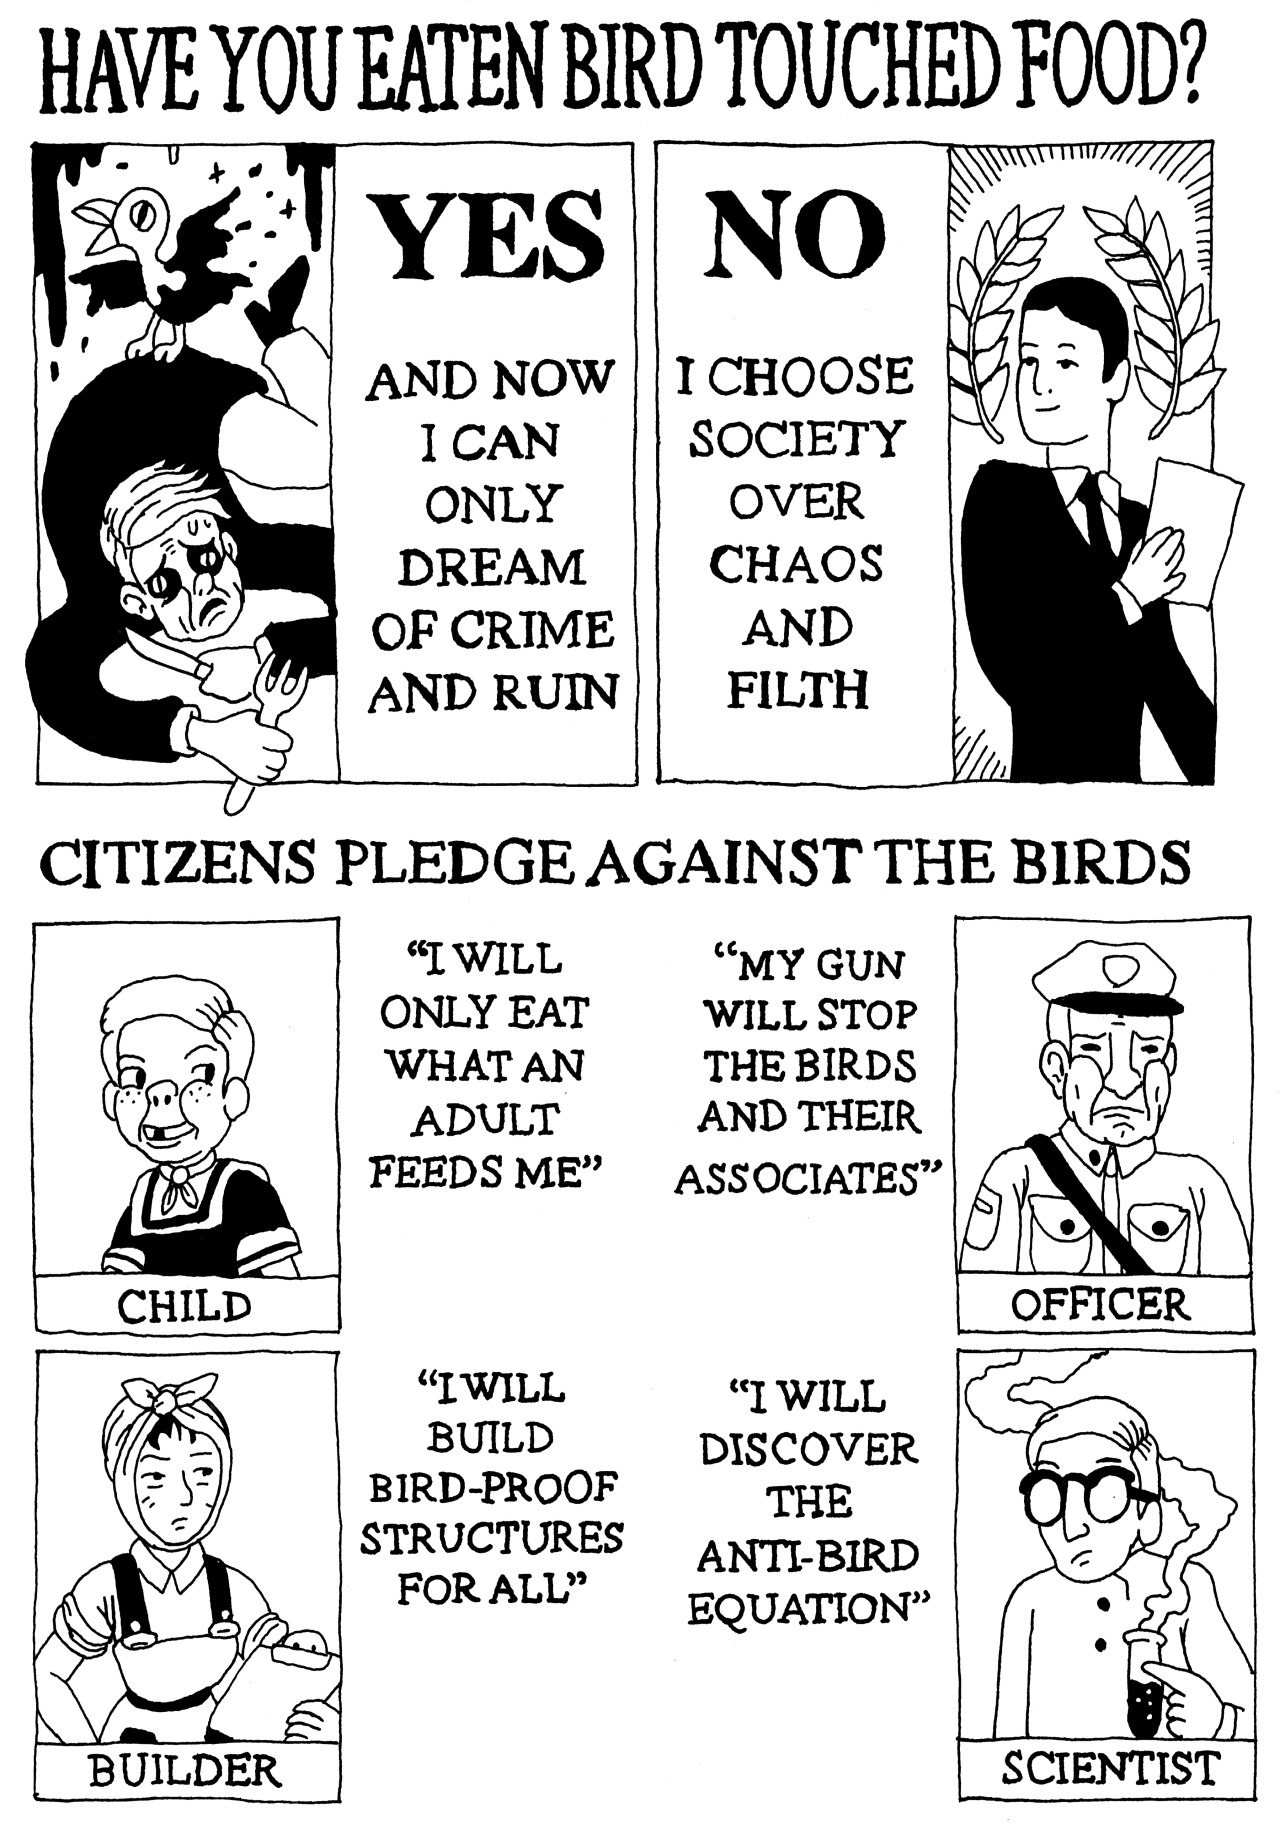
\includepdf[height=7.5in]{assets/4}

\chapter*{Hi, I'm Jack and I'm Not From This World}
\addcontentsline{toc}{chapter}{Hi, I'm Jack and I'm Not From This World}

%\includegraphics[width=5.12in,height=7.6698in]{media/image2.png}

I slap my paw on the table and shout, "And then Bethany says, 'What Sandwich?'"

The entire group erupts in laughter as I finish my story. Kenneth, the elk in front of me, throws his head back so hard that his antlers bump against the wall behind him. My boyfriend wraps an arm around me tightly, and it feels good to have the husky by my side again. It feels like it's been years since I've been able to make people laugh that hard.

The table winds down and a vixen nudges the elk's shoulder, "Hun, you're gonna get us kicked out again."

"Yeah, yeah," he waves his hooves, trying to settle himself down. "I just forgot how funny Jack can be at times."

I know what he means, though only slightly. The waitress comes around, a pug with a tablet out for us. "What drinks would you all be having?" She asks with a perky ring in her voice.

I look up at her with a wide grin. "I'll take a Coke," I say, and then immediately realize my mistake.

So does the rest of the table.

Everyone stops laughing, their eyes all on me. This happens every single time. I get ahead of myself and say something too fast and now everyone is confused. It's like I just unbuckled my pants and shat right in the middle of the table.

"A what?" she asks, turning her eyes to the rest of the group in confusion.

My boyfriend, Tre, touches a paw to my leg and mutters, "Jack?"

I grab my menu, flipping open to the beverages and point at the one on top. "Ugh, sorry, I meant a Pepsi. I'd like a Diet Pepsi," I clarify. It's not actually the soda I want, but it's the only one that I recognize.

The waitress eyes me a second longer before moving to the bear on my left, Dannon I learned. He's my best friend, I think, but it used to be Kenneth. "I think I'll have a Cane," he says, trying to act like nothing is off. I think that's the equivalent of a Coca-Cola, but I'm not really feeling adventurous enough to find out.

Everyone else orders their drinks, and just as the pug leaves, the vixen, Trish I think, asks with her eyebrows raised, "Did you try to order cocaine from the waitress?"

I wave my paws out in front of my chest. "No, no, sorry. I just got mixed up. Don't worry about it," I say, knowing she's not worth the explanation. She's just the flavor of the month with how fast Kenneth goes through girls.

"It's his condition," my boyfriend says, and I fold my ears back. I really wish he didn't, but Tre always likes to explain it so everyone's on the same page. "He was lost in the woods for half a year and so sometimes he gets the names of things mixed up."

She nods her head up and down with some sympathy, and I feel a little guilty cause that's not the truth. It's just the explanation that makes sense to all of them. I kinda hate having to live with the lie, but I put on my smile and wave a paw. "Yeah, what he said. It's not a big deal."

I try to blow past it as quickly as possible and the conversation starts up as normal again. It always feels like a close call, this whole lie I've constructed. See, I didn't get lost in any woods. No, about a month ago, I walked straight into them and knew exactly where to go cause a witch gave me a map.

Alright, none of this is making any sense to you so lemme catch you up. Hi, I'm Jack, and I'm not from this world. I'm from your world, where I graduated from UC Berkeley with a degree in computer science and my favorite football team is the Packers. Not here though.

See, I wanted to go to this world for some reasons I'd rather keep to myself, and in this world I'm not the meerkat that hates Disneyland and loves Buffalo Wild Wings. I walked through a cave and suddenly, I'm Jack that graduated from UC Golden, my football team is the High Kicks, and everyone drives on the left side of the road. That blows, but worth it.

Trish leans in, not wanting to drop the conversation. "You poor thing. What was it like, being out there all by yourself?"

Oh right, and this world's Jack took a camping trip seven months ago and is probably dead. "Harrowing," I say flatly, and that's enough to change the subject.

"We still on for Sunday?" Kenneth asks quickly, wrapping his arm over Trish's shoulder to try and bring her back in.

"Hell yeah! Doug Riot's Wyldstar!" I confirm, and though I'm not actually a big fan of movies, spending time with Kenneth sounds good again. Back in my world, we fell out when I was being a depressed piece of shit.

The bear, Dannon, leans in and taps his big claw on the table. "Uh, actually, I thought we were watching the High Kick's game on Sunday?"

I cock my muzzle to the side, and then slap myself on the forehead. "Aw, shit, I did promise that, didn't I?"

In the month I've been in this world, I've come to learn that Dannon is the guy I hung out with all the time. He's my old college roommate, I think, and kinda clingy as all fuck. I don't know what this dimension's version of me sees in him, but he's been trying to hang out alone and I guess I owe former me that. Heck, this world's Jack could still be out there in those woods and I don't wanna ruin what he had going.

"Let's shoot for Saturday," I promise Kenneth, and he nods. It must be a little weird with me wanting to spend so much time with him. We just seemed to be Facebook, I mean, Faceshare friends in this world.

Tre, my wonderful boyfriend, leans in for a peck on my cheek. My Tre did that all the time too, usually before he wanted to tell me something. I peck him back the way I do. He's the one thing that's a mirror replica, the treasure the witch promised when she helped take me to this universe.

"Don't forget, we're having dinner with my parents on Saturday," he reminds me.

Ugh, they're the same too, but that's no big deal. "We'll figure out something," I promise Kenneth, but he looks a bit disheartened. How the fuck am I supposed to keep track of every new thing, and my schedule. It's kinda a chore.

Saturday rolls around without too much excitement. I only mix up a few things throughout the week, but it's nothing crazy. My coworkers had to wheel me to the correct desk only once, and I call my phone an Android, which makes no fucking sense to anyone.

"Still driving on the wrong side of the road?" Tre's mom asks in the mocking half-joke. half-putdown that she's so good at.

I pour my wine glass close to the brim. "All the way here," I joke, trying not to let her ruin the mood.

Tre's parents are dressed nice, something they like to do when they have company over. He made me put on a dress shirt too, even though I wanted to come in a t-shirt and flip flops. Even between dimensions, some things never change. "It's just part of his condition," Tre says, always to my defense.

I put on my smile and nod up and down. Tre's father coughs and shuffles in his seat. The husky is large and always intimidated me a little bit, but he says in his deep voice, "It's good to have you back, regardless."

I kinda feel like it's a lie. They probably tried ushering Tre towards some bitch the day I didn't come back home. They always wanted grandkids, but me and Tre aren't interested. At least I hope we still don't want any cubs.

"I'm glad to be back. Missed eating real food," I say, patting the little bulge that has grown over my tummy.

His mom snickers at that, pointing over to me. "I bet. You were fur and bones when they found you."

It's true. I stopped eating altogether back in my world, and when I think about it, it wasn't fair to let everyone watch me waste away.

Turning to Tre's father, I quickly change the subject. "How's the firm holding up? Still protecting millionaires from tax evasion?" I joke, something I could do with him from time to time.

It falls flat.

His muzzle scrunches up, brow raising. "Firm?"

Tre's mom leans back into her seat with the wine glass to her muzzle. "Here we go again," she says before taking a loud sip.

Tre darts a glare to his mom and says, "His condition---"

If I have to hear about my condition one more time, I'm gonna lose it, so I interrupt, "Sorry. What is it you do again?"

"State prosecutor. I make sure the millionaires don't evade their share," he says bluntly, and I can see why my blunder rubbed him so wrong.

"And I'm an astronaut, don't you know?" Tre's mom jokes at my expense.

My husky straightens himself out on the seat, saying in a strained tone, "Mother, that's not funny. You're a professor of Biology at Calitazs State."

Biochem at Stanford University, but I'm glad he said it so I couldn't mess that up too. Just little things that're off, and I feel bad for not doing my research. Like a fraud, cause that's what I am. Still, I put on my smile and nod like I belong here because I'm not going back.

I let them do most of the talking and the rest of the night moves on rather smoothly. I can tell that my husky is putting on a show though. There's just something in the way that he talks that lets me know he's getting that much closer to the truth. I need to start doing better.

I arrive at Dannon's house with a six pack of Sunnyvale, and I did my due diligence this time. It's the equivalent of the beer I used to drink, good ol Hefe, so I feel a little proud of myself. "Game day!" I shout as the bear opens the door for me.

He gives a wide toothy smile at my cheeriness and says, "Guess you've been excited about this too, haven't you?"

Dannon leans in, gives me a brush on the whiskers, and I almost pull back. This world's me was a lot more affectionate than I was. I'd never be so intimate with my friends, but I go along with it and brush whiskers back.

"It's the High Kicks against the Calitaza Miners. Of course I'm excited!" I lie.

I'd much rather be watching Aaron Rodgers throw a laser thirty yards down the field, but the High Kick's stallion, Blee, seems to be good enough. Football is football and I'm gonna have fun anyways.

"Yeah, I guess we can watch some sports after," he says as he leads me in.

I laugh cause I think he's joking. Games about to start in ten, and I'm not really sure what \emph{after} is. I'm lead into the living room, noticing that there's no game day snacks, and that's a little disheartening. I'd have at least had some chips out if I was hosting a game.

Plopping my beers on the table, I flop down into the couch and look expectantly at the TV. Dannon seems to know what I'm waiting for, so he takes a seat awfully close to me and grabs the remote. He flicks on the screen, flipping through the channels until he finds what he's looking for.

My eyes grow wide, and I cough out. "This isn't the game?"

No, it's certainly not. It's two foxes fucking like mad. Their moans of pleasure are blaring through the speakers, and the slap of one of the dudes' balls is just loud enough to overcome it. "Oh god, oh god yes," the one getting dicked screams out as he's beating his cock like it owed him money.

"The fu---"

Before I can finish my thought, there's a thick wet ursine tongue deep into my muzzle. It's running up against mine, his lips locked firmly to my face. A paw finds its way into my shirt, claws running through my fur straight to my nipples. I panic and pull back as hard as I can with my paws pushing against the bear's chest.

"Holy fuck, dude?" I scream out, trying to back into a corner of the couch, but not getting far enough.

He barely seems to register my discomfort as he forces another kiss against my lips. "Ohhhhh, I've missed this. C'mere you sweet fuck," he mutters out as he gropes against my leg.

"No!" I shout again, and this time push the big bear back with enough force to throw him down on his own couch. "What the fuck is this?"

The foxes are so loud, I only realize now that he can barely hear me. He grabs the remote with some confusion and hits pause on the TV. I'd rather he just turn off the damn thing, cause now it's stuck on a close up of the foxes railing. Dannon says with some puzzlement.

"What we always do when you come over for the game. Or is this part of your \emph{condition}?" He asks with a grin.

"Maybe? Yes? I don't wanna fuck you, if that's what I've been doing," I spit out quickly.

``Jack, you can drop the act. It's just me,'' Dannon says, and my heart sinks in my gut. He lets out a low lusty growl, desire still in his eyes. "You joined some sex cult out there in those woods. Got into the really freaky shit, didn't ya?''

I'm a little disturbed, but mostly relieved he's wrong. ``You're always wanting to hang out with Kenneth nowadays. You fucking him too, little slut?" he asks, and not maliciously. It's twisted. Like I'm supposed to be getting off on the idea of fucking around behind Tre's back. Like I probably did.

He's not reading me right at all, and he leans in again to run a claw right up my inner thigh. I hate it, because I know he knows exactly where to touch me. Only my Tre knew that spot. Blood rushes to my groin, my body betraying me. He doesn't get to touch me like that again.

My fist swings wild, knocking him right on the nose. It sent the message home as he completely rolls to the other side of the couch. Paws are clutching his muzzle and I can see blood pour between his fingers. He says something like, "Fuck! My nose!" but I can't really make it out when slamming his front door behind me.

I stomp towards my car, fist still clenched tightly. I practically scrape up my paint job trying to get the keys in the door. As soon as I get in, I'm out on the street. It's not until I almost run head first into another car that I realize I'm on the wrong side of the road again.

There's a few blocks difference between me and Dannon's house before I pull over. Guilt builds up in my chest for hitting the bear the way I did. He should have stopped when I told him too, but I wasn't as angry at him as I am myself. This other me.

How did he not know how special Tre was? How could another me have taken his husky for granted like that? He couldn't have understood the lengths I've gone to get back to Tre. A bad thought crosses my mind, glad that this world's Jack went missing. It's not good, because I don't think anyone deserves to die.

I want to go home, but I can't. It would look too suspicious and I got the jitters anyways. I'm such an awful liar, I have no idea how Tre hasn't found out already. My first thought is to go to a bar and watch the game there, but football is ruined for me at the moment. Then I remember Kenneth, my actual friend.

The elk agrees to see Wildstar with me. I'm glad that we can just sit in the cool movie theater. It gives me time to collect myself. The explosions distract me, and by the time we walk out, I'm feeling a little better. Kenneth points at a shop, some chain called BlueTops. It's sorta like Starbucks where I'm from, but everyone drinks hot cider instead of coffee around here. I think it's gross, but I do wanna chat with him, so I agree.

"How was the football game?" Kenneth asks casually, and it's a little bit of a surprise to me.

"Oh, uh, I didn't end up watching it," I say, and I guess with us not being friends in this universe, he wasn't interested in football, else he would have known that. Maybe I should have asked my Kenneth if he ever really liked watching the games with me.

He cocks an eyebrow and asks, "Did something happen with you and Dannon?"

There's a lump in my throat. I want to tell him everything, the way I'd tell my Kenneth, but he's not him and I don't want to dump everything on him. "I don't think I want to hangout with him anymore," I admitted, and that was mostly the truth.

He nods, pulling up his cider to his muzzle and taking a sip. There's a little bit of an awkward silence so I blurt out, "How's things with Trish?"

The elk snorts, the steam coming off the drink blowing all over the place. "We split up. She had too many issues with my rack, and truthfully, I wasn't a big fan of hers either," he said, waving his hooves in circles.

I laugh, "Same ol' Kenneth. Always on the hunt for something better." As I finish, I take a big sip of my cinnamon apple cider and try my best not to wrinkle my muzzle. I don't know how they do it here, but they replaced ketchup with buffalo sauce, so, I guess it's a fair trade.

His brow goes up, but his smile doesn't fade. "You say that like we know each other. This is the most I've seen you in years," he states, though it's not a challenge.

"Why did we never hang out? You're awesome," I say, because I'm still not sure what happened in this universe.

He scratches his chin with his hoof, looking at me shyly. "I guess I never was your type? Your friends usually seem to be more your speed," he says carefully, skirting around the issue and it finally clicks with me.

I wasn't--- this Jack wasn't friends with someone unless they were sleeping together. And it was a dirty secret that everyone knew. Man, I was such a loser in this world cause Kenneth is the best. Well, I guess I am a loser in my own world too, cause I let my Kenneth go as well. That wasn't going to happen again.

I lean over and say with a smile, "I'd like us to spend time together more. You watch football?"

Coming home, I'm feeling a lot better. Kenneth agrees to come over next Sunday so I can teach him about the game. I also make a note to pick out some movies to watch together, because this Kenneth seems to enjoy doing that. No foxes fucking on the TV this time. I open the door to my house, and hear Tre call me from the basement.

I get to the top of the stairs and knock on the open door. "You down here babe?" I ask, slowly descending the steps.

"Yeah! Come down here. I wanna show you something," he calls back, and I can hear him fiddling with things.

It's dimly lit down here, and I can see him in a corner with some bikes on the rack. "What're you up to, hun?"

He doesn't turn around as he continues messing with the bikes. "Just looking at old pictures of us at Cinderland. We look so goofy in the photos. You remember that?" He says chipperly.

Ugh, another thing different. I know Cinderland enough from the ads to know it's Disneyland and I hate that place. Not only was this me a cheating bastard, but he was also one of those Disney nuts. I'd never willingly go to that shithole. I roll my eyes and put on my best smile.

"Oh yeah. That was a lot of fun. Can't wait to go back," I say, and it's hard for me to keep that same cheery tone.

"Photos in the desk," he says, but his voice sounds a little different.

I turn to the desk, and it's not my Dad's cherrywood, but a blocky metal workstation. I pull open the long drawer handle and freeze as I see nothing inside at all. I turn to face the husky and say, "Um, hun, there's nothing in--- oh."

Whelp, this is different. My Tre didn't own a gun. But now this Tre was pointing one right at me, paws shaking. Tears are running down the sides of his face and his muzzle is twisted in an angry frown. "Hun---"

"Don't you fucking \emph{Hun} me. I don't know who you are, but my Jack would never go to Cinderland. My Jack hates that place, but you wouldn't know that cause you're not him," he says, legs spread like he's bracing himself for the gun to go off any second.

My heart's pounding, and I slowly raise my paws over my head. He's shaking so bad, it's just as likely he's gonna shoot me on accident as much as he is on purpose. Not gonna lie, but a little wee comes out. "My condition---"

"STOP IT," he barks, thrusting the pistol forward. "Stop lying! You're so fucking bad at it, and I'm done lying for you."

He's been taken way past the edge, and It's killing me to see him so distressed. I should've known he could see right through me. My Tre always could, and I shouldn't have expected any different.

"It's not what you think," I start, my heart breaking as I'm forced to admit the truth. "But I'm not your Jack."

"I knew it! I knew it from the start that you weren't him! And you just lied to me and took advantage of me," he says, fang sinking so hard in his lip that he's drawing blood. "Who the fuck are you? What the fuck are you? Are you some furwalker? Some sort of demon?"

I gulp loudly and try to explain all at once, "I'm Jack, but I'm not from here. A witch gave me directions to this cave where I---"

"I swear to God," Tre says, and grips his pistol tighter.

My muzzle cracks, I can't hold anything back because I don't want to say it. I don't want to relive it. The lengths I've gone to escape that hell. I don't want to say it, but he deserves the truth and so I shout through a sob. "It was you!"

His maw opens and there's a look of complete puzzlement on his muzzle. He's about to speak, but I snort up snot and explain. "Where I'm from, you went on that camping trip seven months ago. Not me. And when you left you just---" I choke down mucus building up in my throat. "You just vanished"

"I spent months in those mountains looking for you. Every time the rangers went out, I was there. All the money we saved was spent on private expeditions when everyone else gave up. I stopped eating. I stopped sleeping. I stopped talking. People couldn't even stand to look at me anymore. I got so desperate, I started going to psychics and paranormal shit for help. Anything just to have you back."

I fall into the workbench, and drag the back of my paw over my eyes. He's barely visible through my tears. I can tell he's still got the pistol out, but it's pointed slightly downward. There's a small sniffling as he tries to work out everything I've said.

He shakes his head back and forth before he says, "It scares me like nothing else. Since you've been back, you've told me nothing but lies." I brace myself, thinking it might be it for me, but he finishes, "You're such an awful liar, but I think for the first time, you're telling me the truth. Or whatever you think the truth is."

I let out a small sigh of relief and hold out my paw towards him. "I'm sorry I lied, but I'm telling you the truth now and truthly, I want you to put down the gun so we can just talk about this."

Tre looks down at the pistol like he hadn't realized he'd whipped one out on me. He scoffs, rolls his eyes, and then tosses it my direction. I panic, floundering as it goes sailing through the air. I cup out both paws, bracing myself for it to go off and take a finger with it.

It clanks softly against my paw pads, lighter than I expect it to be. Only when I feel the slosh of water do I realize that it's not a real gun. In fact, looking at it close up, it's pretty obvious it's a squirt toy. I look up at him and he takes a step back, ears red hot with embarrassment.

The husky's lip is quivering as he whispers, "I'm sorry. All I wanted was the truth."

I set the squirt gun behind me, but I'm a little afraid to approach Tre. His muzzle is to the ground, like he did something wrong. I mean, it wasn't very nice that he pointed a gun at me, but I guess I kinda had it coming.

"Sorry, for all the lying. I thought if I stayed here long enough, you'd never notice," I admit.

He rubs his eye, letting out a small pitiful laugh. "You've always been a bad liar. He was always a bad liar too: About Dannon, the other guys, football, and all that."

My ears go up, and I feel some collateral guilt from what he just said. "You knew he was cheating on you? And you stayed with him anyways?"

His legs wobble before he can't even hold himself up anymore. He takes a weary step back, thumping against the wall and slowly sliding down it. When he's on the floor with his head between his knees, he says. "I knew. You used--- he used to think he was so sly, but I always knew. He wouldn't even know the scores when he said he was out watching football. But I stayed cause losing you--- him---"

He pauses to look up at me, and I feel connected with him in an awful way. The way that I never stopped looking in those damn woods. I gave up my friends, my life, my family just for the sheer hope of seeing him one last time. What we shared was the inability to let go, and I see it in his eyes like he sees it in mine.

"I guess it doesn't matter anymore," he starts, waving a paw lazily around. "I lost him anyways, and he's never coming back."

It's the words he needs to say, just as much as the words I need to hear. Cause truthfully, my Tre is gone too. My Tre is never coming back. For the first time ever, I have to accept that. So I walk over, pick a spot close, and get down on the ground with him.

It feels like we just stay there in silence for hours. Maybe it is, because there's a million things for me to think of doing next. I could probably go back and find that cave again. Repair things with my Kenneth, make things right in my world. Not everyone gets a second chance like this, so instead I say.

"I don't know what happened to your Jack, and I don't know what happened to my Tre. They just disappeared, and I don't think they're coming back," I say, then lift my head and turn towards him. He's done the same, and our noses are just a few inches from each other. He's not crying anymore, though his eyes are red.

"But what I do know is that you're the only Tre I have left, and I think I might be the last of me that exists. So how about this?" I gulp, and hold out a paw towards him. "Hi, I'm Jack, and I'm not from this world."

He laughs, cause it does sound a little goofy. I could always make my Tre laugh unintentionally, and it gives me confidence I can make this one laugh like that too. He doesn't take my paw yet, so I continue, "I like Buffalo Wild Wings, though, I have no idea what you call it here. I hate Cinderland, but we call it Disneyland where I came from"

"Kenneth was my best friend, and I didn't hang out with anyone named Dannon. I actually watched football when I said that's what I was doing. I wasn't perfect, but not once did I ever cheat on my Tre, and I promise I would never cheat on you either," I say, and it starts to make my eyes water thinking about the things this Tre has gone through.

He looks at my paw, thinking about it for a minute, before his eyes turn up to mine in a stern look. "No more lies?"

It's a big promise to keep, but I've gone too far to turn back now. I nod and repeat, "No more lies."

With a sigh, he reaches out and clasps my paw. "Hi Jack. It's nice to meet you. My name is Tre. Welcome to my world."

\cleartoverso
\includepdf[height=7.5in]{assets/9}

\chapter*{Tribute to the Basking God}
\addcontentsline{toc}{chapter}{Tribute to the Basking God}

%\includegraphics[width=5.01563in,height=7.518in]{media/image8.png}

Olin sat with himself, twining together bishop's lace flowers. The otter was careful to string the green stems, spacing out the white pedals equally along the bracelet he was making. He wanted it to be perfect. It had to be if it was going to be for the Basking God.

He looked up from the boulder he was sitting on. Between the trees, he could see the Basking God doing what he did best. The coyote was on his back laying the grass, staring up into the clouds. At least, it appeared so, though it was hard to tell with the visor he wore over his eyes.

He wasn't sleeping, that was for sure.

Three other otters, all women and a third his size, were on top of him. He made no moves as one rode his cock, not suppressing any of her moans. Her hips went up and down, the full length of his rod inside of her pussy. The other two had sat on his paws, squirming delightfully at either of his sides while his fingers played with their delicate flesh.

It was common for the ladies to be adorned with The Basking God's blessings throughout the day. Mated or not, he provided all the women of the tribe with his gift. The men held no jealousy. In fact, they treated it as an honor to share their partners. Afterwards, they would listen as they would share their love making with the Basking God.

One of the otters being fingered was outright panting, muttering words strong enough to hear, "My Lord. My God! I'm approaching."

The Basking God grunted, and said through gritted teeth, "Never\ldots confirmed nor\ldots denied." It was something he always said whenever someone referred to him as a God. He was a modest deity, something Olin admired in him, even though it was clear he was a god.

She flung her head back in her third or fourth orgasm today, crying out in pleasure so loud that it echoed in the forest. The Basking God had a small smile across his muzzle, pleased to participate in their worship.

Olin's cock was hard underneath his white tunic. It was distracting him, and though he wanted to please himself, he had more important matters. Tomorrow was his day of age, the day where he would finally be allowed to take a maiden and please her the same way the Basking God would. But he had no interest in doing that when he had a god in mind.

A feminine voice came suddenly behind him. "Enjoying the view?"

Olin nearly leaped out of his fur. His head twisted back and he came almost nose to nose with his sister, Leia and wrinkled his nose back. "What're you doing here?" he asked defensively, more startled than angry.

She shrugged lazily, lifting her nose towards the trees. "Same as you, I suppose. Tomorrow is a big day for both of us," his twin said nonchalantly.

Olin rolled his eyes, and in his brief momentary forgetfulness, she peeked at his bracelet. "For him?" she asked curiously.

"Shut," Olin hissed, trying to hide the bracelet to no avail. Then he quickly recovered. "Irani. It's for Irani." He only named the first girl off his head.

Leia nodded and crawled up onto the boulder with him. She sat thoughtful for a second and then peered up at The Basking God. Her gaze lingered on him and the other otters as she spoke, "You know, it looks really good so far."

Olin looked down on the flowers he was twining, wondering how true that could be. He had confided in her when they were little of his love of The Basking God, but had gone quiet about it the closer he got to his day of age. She hadn't forgotten. When he turned up to her, he asked with some reservation, "Will it be good enough?"

Leia leaned in gently and brushed her whiskers to Olin's. He returned the affection, as awkward as it was while still stiff. Her giggle might've told him she knew, but she pulled back and kept her eyes to his. "That's up to the Gods," she said playfully.

"Pff, some help you are," he said, giving her shoulder a nudge of his own.

She pushed back with a wry grin. "I dunno what you want me to say? He's ancient. Rode in from the stars generations ago only slightly after the great exodus. It's hard to tell what he would do or think if you asked him to be your mate."

That was true. At least, if the stories were true. They say there was the mountain god before him, and one day the mountain had gotten angry and spewed hot liquid onto their village. Angels intervened, scooping up the survivors and brought them to this island paradise. And then the coyote came afterwards, and all he ever wanted to do was bask.

Leia, seeing Olin stuck in his own head, waved a paw in front of his muzzle and said, "Don't overthink it. He's kind. He likes you well enough. I don't think he'll get mad and," she paused to give him a quick peck on the cheek. "I don't think any of us will be mad either."

He returned the peck and she got up off the boulder. Leia gave a small bow and Olin put himself back into his work. By the time he finished the bracelet, the girls were done. All three lay spent, curled up all around the coyote and grooming him. One was busy licking him clean of her juices, while another had taken to massaging his feetpaws. The last was busy feeding the god grapes that she had brought as her tribute to him.

All three chittered away casually to themselves, the coyote mostly remaining out of their conversation. It pleased him to just listen, giving only small nods whenever he was included in their gossip. Everyone in his tribe of a hundred or so appreciated the Basking God for his tranquility. He was a kind and very giving deity.

A chirp rang out from the coyote's bracelet, one of his magical devices. Only The Basking God was allowed to use them, but he was forgiving enough when the otters would examine his trinkets curiously. He turned his bracelet to his muzzle and gave a couple clicks of his tongue. All three girls were off him, and then they feebly tried to help him off the ground. The coyote was too large for them to assist much, but they patted his nude figure from dirt and grass that had collected on his fur.

"Easy girls, you'll have more of me tomorrow," he chuckled, giving them all pets along their muzzles. They fell into a giggle fit, each of them taking a turn to kiss his extended paws. The god gave a stretch before saying, "It's story time."

Olin's thick otter tail slapped against the boulder behind him. He loved The Basking God's stories, almost as much as the coyote himself. The coyote had endless adventures that no one else could provide. The otter had often imagined himself being able to go on such a journey. One with villains and heroes and monsters, but there were none on this island paradise. All he had was the Basking's gods tales.

It was enough though, but when the otter tried to get up off the boulder, eager to join everyone in the amphitheater, he felt his erection slide against his tunic. Quickly, he was back on his butt, feeling a little flush with embarrassment.

He could trust that it would subside by the time he arrived back to the rest of his village, but he didn't necessarily \emph{want} to do that. After having watched the coyote please three of his tribe members, Olin was feeling eager to please himself. Everyone would be working their way towards the amphitheater by now, though no one would mind him if they caught him masturbating. All were free to pleasure themselves in the realm of the Basking God.

And so Olin did.

The otter placed one paw on the boulder, lifting himself as he pulled the belt off his tunic. Olin unwrapped his clothing, spreading his legs and sitting back down on his bare ass. His lower half exposed, he reached a paw down and grabbed hold of his member. It wasn't nearly as impressive as the Basking God's nine inch canid rod, though he wasn't too small for his size. In fact, he was quite endowed for an otter.

He began to pump all five inches of his cock up and down. Olin squeezed his eyes shut, nostrils flaring as he took in quick sharp inhales. He didn't realize how pent up he had been from watching the Basking God work with the girls. Picturing in his head, he imagined if he was one of them sitting on the coyote's paw. With a wet slurp, the otter shoved two fingers into his muzzle and slickened them with his spit. Carefully, he brought his paw to his behind and touched it to his tailhole.

Ever since he had gotten his urges, he had fantasized about joining the Basking God in his court. He'd only ever seen him with the tribe women, but he could imagine himself as the first boy to be with him. Olin pushed his fingers inside, picturing the coyote pushing one of his large claws inside of him. Just the thought was enough to have him squirming and whimpering to himself.

There was no one he wanted more than the Basking God. None of the otters came close, even the other boys. Olin wanted to feel small and vulnerable to the coyote. He wanted his god to handle him, use him however he wanted, whether that be mounting his backside or deep throating that massive canine cock of his. No matter what his god asked of him, he would do it happily.

The thoughts were enough, the otter coming up past the point of no return after barely two minutes of stroking himself. Olin plunged his fingers inside of himself, even trying to wiggle in a third just to better imagine it as the coyote's. He let out a muffled moan before he was caking himself in strings of cum. His orgasm was intense, almost blinding. His eyes rolled back into the back of his head, and soon his entire consciousness was only the sensations of his climax.

Olin's chest slowly stopped heaving, and he had to blink himself back to reality. He wasn't sure how long he was laying there relaxing with a pool of cum drying on his tunic, stomach, crotch and paws. It felt relaxing and he knew it was going to be ten times better when he actually experienced it with the Basking God.

The otter gasped, practically jumping off the boulder and scrambling to find his belt. He was missing story time! He'd missed, maybe, only a handful of the coyote's nightly stories. Quickly, Olin rushed to his own hovel, putting on a new tunic and racing to the amphitheater.

If Olin could have made a scene, he would have screamed and thrown himself on the ground like a little cub. Tonight, the night before he was to approach the Basking God, every single seat in the amphitheater had been taken. Of course, it was always packed, everyone wanting to listen to the coyote's tales. Just usually he was the first to arrive, getting a spot in the front center.

Instead, he had to stand in the back and watch from afar. Despite that, The Basking God noticed Olin, or at least had noticed his absence and gave a small wave to the otter as he stepped in. The pause in his story was small, hardly noticeable to anyone else, but to Olin, it made his entire body hot with embarrassment.

The otter quickly found a spot to stand, leaning back against a wall and trying not to bring anymore attention to himself. Thankfully, he'd only missed the recap of the previous night's story and not much more. The Basking God quickly picked up where he'd left off yesterday. Naked on the stage, the coyote loomed over and spoke.

``Just before Neo could return to the mortal plane with his mentor and friends, an arrow flew right at him, striking the portal door and destroying it!'' ---As the coyote spoke, he performed the role of Neo, ducking underneath an imaginary arrow and looking in horror behind him--- ``With the door closed, he turned back to see that the automaton, Agen Smit walking into the tunnel.'' The Basking God moved himself to the other side of the stage, ambling forward calm and steady as he continued, ``Mizdar Andarson, the automaton said, taunting Neo by referring to the name he no longer recognized.''

Gasps and cries from the audience rang out, and even Olin was getting caught up in it. He remembered the description of the automaton from last week: a soulless being that could rebirth itself at will. Several listeners reached their hands out, shouting for Neo to run, and it took all of Olin's willpower not to cry out as well. As if answering, the coyote held a paw up to the crowd and retook the role of Neo.

``No, he would not run. For if he was truly The One, then it could no longer be proven by words alone,'' The Basking God said, drawing an imaginary bow. ``If Neo was to believe the prophecy, then it would have to be proven with actions" ---The coyote released his bow, whistling just as he pretended to dodge an arrow himself--- ``The two fired their arrows at close range from one another, moving so fast that both were only just able to dodge the other's shafts while drawing from their quivers.''

It was like the coyote was dancing on stage moving his arms out elegantly while he pretended to fight. Olin pictured the two of them inside his head as the Basking God swung in long motions across the stage. His maw was open, wide eyes drinking in the scene.

``Neo reached for another arrow, but his quizer was empty!" Another round of gasps from the crowd, but The Basking God continued. "The automaton taunted him. 'You're out', but with a wry grin, Neo said, 'So are you.'" The otter's cheered at that and then the coyote had quickly pretended to fight an imaginary figure on stage as he spoke, "The automaton's strikes were so hard, he could punch holes through pillars with just his bare fists. Neo landed a thousand blows across Agent Smit's body and hundreds of kicks, but nothing could stop the monster.''

Now some in the front row had become hysterical, crying out for Neo loudly. A couple otters were even pleading for the automaton to show mercy, but Olin knew it wouldn't show any. He couldn't help but feel a little embarrassed, wondering if he ever reacted the way they were while in the front row. He knew he probably had, and probably would have been acting the same if he was up there now.

The Basking God got into a crouch position, wrapping an arm around an imaginary figure's neck in a chokehold. ``\,`You hear that, Mizdar Andarson?' the automaton said, looking forward towards a tunnel's entrance'' ---The coyote began to wrap his knuckles against the ground in a steady trot--- ``\,`That is the sound of inevitability.' Adain Smit said, watching as a steel chariot was moving full speed their direction.''

Olin leaned forward, heart picking up pace. He didn't think this story would be a bad story, but he couldn't see a way for Neo to escape. Only during the end of the harvest would The Basking God share scary stories, and it was only the start of the year. Without thinking, Olin shouted from the back, ``Get up, Neo! You need to get up!''

People joined in, crying out for Neo to fight the choke hold. The Basking God was cruel, his knuckles wrapping faster and faster on the ground, the chariot drawing closer from the tunnel's entrance. Just when the audience was screaming louder than the coyote's gallop, he flung his arm up into the air, silencing the whole crowd. Then, he took position back onto the floor and resumed the end of the scene.

``Neo, at the last second, found his foothold on the ground and turned his muzzle to face the chariot. Then he said to the automaton, `My name\ldots{} is Neo!'. With his superpower strength, Neo jumped up from the ground, hitting Adain Smit's back against the ceiling,'' the coyote said, and then tried to perform the leap as best he could. It wasn't nearly as impressive as the backflip The Basking God performed immediately afterwards, and everyone could visualize Neo barely escaping.

``Swhoosh!'' he said, whisking his arms in the air back and forth. ``The chariot just narrowly missed Neo, while the automaton was crushed and swept away underneath its wheels!''

The entire amphitheater was roaring. Olin was part of it, if not the loudest in the back. Everyone was stomping their feetpaws and thumping their tails to their seats. The Basking God waited, and the sly smile on his muzzle settled the crowd. When the otters had mostly subsided, he picked up the story. "But the chariot only made it a small distance, not even out of the other side of the tunnel, before the wheels came to a halt."

There were murmurs of confusion whispered between ears, but The Basking God didn't wait for them to settle. Instead, he held up his paws and said, "Next time, we will see if Neo truly defeated the automaton and how he plans to escape the dream worlds back to reality."

Applause erupted for the coyote and he bowed deeply in gratitude. He was such a humble god, even when they adorned him with gifts. Several had rushed the stage, presenting platters of food for him to take. He grabbed a small morsel, taking it into his muzzle as he helped himself off stage towards the communal eatery.

Olin followed along, taking his normal spot, but mostly remained to himself. Even as his friends prodded him with questions of tomorrow, curious queries and suggestions for ladies to pair with. He waved them off, and they mistook it for sheepishness. Though he was shy, he didn't want to tell them of his plans. His judgment would be passed by The Basking God alone.

Though he hoped to be well rested, Olin found little sleep during the night. Thoughts of the coyote kept him turning left and right, as well as a pestering erection. It took all his willpower not to finish himself, hoping to be fruitful for The Basking God. First thing in the morning, he would find out if his restraint would be worth it.

Unfortunately for Olin, rest came late, and so with it, he found himself waking up to a high sun. He scrambled out of his hovel with his tunic half on and a satchel flinging about his side. When he raced towards the grounds of The Basking God, he was relieved to not see anyone with the coyote. As always, the canine was doing what he did best: Basking in the sun.

Olin saw him half dipped into the river. Again, his strange visor was over his head and he was staring up into nothing. The otter started with a quick pace, turning behind him to make sure nobody was following. At first, he thought the coyote did not notice his presence. The closer he got, the more pregnant the pauses in his step became apparent.

When he was ten paces away from the deity, he watched his canid ears flick his direction. Without even turning his head, the coyote brought an arm up and waved him forward. His voice was bolstering as he said, "Olin, my friend! Such a good day to see you."

The otter froze, heart constrained in his chest. It was always awkward and flustering whenever The Basking God called him by name. Of course, he knew everyone's name in the village, but it felt like he should have been above it. Meekly, Olin closed the distance with his satchel in front of him.

"My Lord," Olin started, opening his bag with fumbling paws.

The coyote had a smile and a slight wistfulness in his voice as he said, "Never confirmed nor denied."

Now, The Basking God had shifted slightly, half of his body still in the water. He turned to face Olin, pulling up his visor so he could make out his muzzle more clearly. There was a sly grin curving the side of his muzzle and he looked as if he knew what was on the otter's mind.

Before Olin could speak, the coyote gandered a guess, "You were late last night to my stories. I'm guessing something with your day of age kept you occupied?"

Olin's muzzle went hot with embarrassment, and he gave a small nod. The coyote returned a small chuckle, shaking his head. "You've always been a bright, thoughtful young boy. Any maiden would be lucky to have you, don't you think?"

There was a twinge that coursed through him, but he managed to steady himself enough to draw from his bag. The coyote peeked his muzzle at a package, seeming curious as he asked, "Is this a tribute to the Basking God for a blessing?"

Olin nodded, opening it to reveal the salmon he'd traded the day before. It was only the finest cut, salted and stored with care. White marble lined criss crossed over the pink meat, and it was the thickest he could barter for. He presented it to the coyote who took a piece and indulged.

His eyes seemed to water as he savored the melting meat in his muzzle. He even caught a moan leaving his lips, and the god smiled widely. When he swallowed it all down, the coyote said gleefully, "Well, I feel the one blessed with that. Truly, you spoil me."

Olin ducked his head, and the coyote caught it. Quickly, the Basking God raised a paw. "No, no. I mean, I bless you and your endeavors, Olin. But you seem nervous. What bothers you, friend?" The coyote said, trying to get himself in a better position to talk.

The otter gulped, feeling strength in the coyote's blessing. Hopefully it would be enough. Cautiously, he pulled the bracelet from the satchel and handed it over to the canine. The Basking God took it and looked it over with some confusion, only stating in a question, "If looks perfect to me?"

Then Olin stepped forward, trying his best to convey his offering. A light seemed to flash behind the coyote's eyes and quickly he realized what was being presented to him. He said with a wry smirk, "Olin, you know this is supposed to go to a maiden, right?"

Bashfully, Olin pulled his paws back and his worries seemed to get the better of him. He had a thought to run to his hovel, grab as much as he could, and forever leave his tribe shamefully. Before he could, The Basking God noticed his dread and said, "No, I guess it's not supposed to go to a maiden if it were made for me."

With tears building up in his eyes, Olin watched the coyote take the bracelet from his paws. He examined it for a second and then slipped it onto the same paw as his bracelet. The canine turned his wrist around back and forth, looking over it with a smile and said, "It's perfect."

They were mated.

Then, with a grunt, the coyote reached into the river, doing something Olin couldn't see until he brought an otter out with him from the water. It was Leia, nude with a shit eating grin on her muzzle. The other twin frowned, should have suspected that she would have gotten there before him.

Sensing his displeasure, Leia brushed the back of her wrist across her muzzle and said teasingly, "What? I was just getting our God prepared."

The coyote seemed to take some pleasure in this, pointing a finger up to interrupt, "Never confirmed nor denied."

His sister crawled up the coyote's stomach, then up to his chest to nuzzle underneath his neck. Olin turned his head away, her naked form a little too much for him. She kissed at the bottom of the coyote's chin, and when Olin thought to just turn around, a massive paw reached out and grabbed his arm.

Olin squeaked as he was pulled towards The Basking God. The coyote let go and scooped underneath the otter's tunic, feeling up his bare backside. His entire paw was large enough to hold him, the sensation sending shivers running up where he touched. His fur bristled through his tail and all the way to the tips of his two round ears. He let out a gasp in pleasure, along with some loving chirps.

Olin didn't seem to know what to do with his paws, both clutching into the air at nothing. The Basking God was more than happy to direct him. "Aren't you wearing a little much to show your devotion?" he asked with a laugh.

Flustered, Olin felt it was more order than suggestion. He grabbed his belt, undoing it and then pulled off his clothing. Part of him wanted to be dignified, folding the tunic beside The Basking God like the other women would, but the coyote seemed to want to get things started now. All he did was toss them to the side, erection clear as day.

His sister turned her head, looking over Olin with an impish smile. His muzzle grew hot, and he almost wanted to tell her to look away. Still, this was the Basking God's grounds and it was common for sisters to please themselves with their siblings. That thought settled him some, and he relaxed a little.

The coyote, seeming a little impatient, gave a motion towards his crotch still underneath the water. Olin nodded, the paw on his rear coming loose. With a running start, he took a breath a lept into the water. His dive was perfect, as well as any otter could.

Olin spun around in the river, feeling the current pulling him away. With his thick tail and paws, he swam towards The Basking God. The water was crystal clear and he could see the coyote was seated on some rubble underneath. Above that was his red erection, eager for worship.

The otter swam cautiously close to the rod. He knew he could hold his breath for a long long while, not needing to come up until the coyote was satisfied. Carefully, he placed one paw on his leg, pulling himself so his own erection rested on The Basking God's knee. Then he wrapped a paw around his shaft.

Despite the water being cold, his canine cock was extremely warm. He pumped at it curiously, studying the flesh with his touch. Never before had he held another man's erection, and this was a big one to start with. The Basking God's member was about half of his own height, and his small paws couldn't even grasp half the circumference of it.

Olin wrapped his legs around The Basking God's, keeping himself from being carried away by the current. Then he grasped at his cock with both paws, giving it a nice long stroke up and down. He couldn't hear if he was enjoying it, but the salty change in the water told him he must've.

The otter got down to business, pumping his cock long and slow. He made sure he was steady, knowing exactly how he would have liked it if he was doing it himself. All nine inches of the canid shaft twitched underneath his paw pads. A palm swooped into the water, nuzzling against the back of Olin's head appreciatively.

Remembering how the girls would please the God, he pressed his muzzle against the shaft. The warmth felt good, and he kneaded at it lovingly with his whiskers. An added intensity to the scritches at the back of his ear encouraged him to go further. He kissed along the side of his cock, and followed it with a few small licks.

Even under the water, he could hear The Basking God let out a loud coo of pleasure.

With only small hesitation, he lapped his way up to the tip of his cock. The canine crown was pointed, the saltiness strongest at the head. He tested a slow drag of his tongue around it, circling it like an otter would its prey. He ended with a follow up kiss, and he felt like he was truly a worshiper now.

Olin wasn't sure if he was capable, but fitted his maw around the tip. He couldn't take in much, but he wrapped his lips around what was in his mouth and began suckling. That sweet nectar poured into his muzzle, and he gulped it down greedily. His tongue swirled around the length, eager to taste every inch of his god.

Before he could enjoy himself too much, there came a gentle tug at his ear. Olin ignored it a second, wanting to continue pleasing the coyote, but a sharper pull told him he was needed. He heard The Basking God call his name, though it was soft as ever, like a parent rousing a child.

When Olin got back to the water's surface, he was almost met with his sister's flesh in front of him. She was in the middle of climbing off his chest, standing on the ground next to him. The Basking God was looking down with a wide devious smile on his face and Olin matched it.

This was it. This is where the Basking God would take him like he had thousands of times with hundreds of women. He wanted it so bad, wanted to be filled with his love. Olin had been practicing often with his own fingers and some smoothed figures, and he was sure he could take it.

"Olin, I've been waiting for this day for a very long time," the coyote said, and it made his heart flutter.

"Yes. Please yes, my lord. I want to ride you and moan with my sister," Olin said, excitement in his devoted words.

The Basking God's muzzle twisted and he said with an awkward smile, "Oh, uh, actually." He paused, and turned his entire body, almost throwing the otter off his crotch.

Olin was unsteady, still in the water and having to swim back towards the coyote. He didn't understand. The Basking God was now leaning on his front, his backside in the water and his crotch towards the ground. He grabbed hold of his tail and flicked it to the side, presenting himself to Olin.

"I was hoping you would take me," The Basking God said, a nervous chuckle following behind.

Olin's eyes widened and he buttered out, "Mount a God?"

The coyote lifted a paw, finger pointed upward in a halting motion. "Never confirmed nor denied," he said, as always.

Now there was something distinctly mortal about the coyote. He had an eagerness to the way he presented himself. "Well, you're not gonna make me beg, are you?" The Basking God joked, but in it, there was an actual neediness to his words.

Olin gave his muzzle a shake, snapping himself out of his own head. He stood in the water, the lower half of the coyote dipped enough for him to line up perfectly. With a gulp, he pressed his member between the perfectly plump cheeks and asked, "It'll be fine?"

A cackle flattened his ears, but The Basking God followed it with, "No offense, Olin, but I think I'll be fine. The water should be enough and I've had\ldots let's say, bigger in me."

Olin wondered what The Basking God could mean. No other men in his village had ever mentioned mounting the coyote before. He was beginning to question the coyote's divine status, especially when the coyote turned back again, tongue hanging out of his muzzle in a pant. Still, he pushed forward, and felt his cock pierce his hole.

His cock dragged slowly against the inner ring of his sphincter. The water was enough lube for him to enter easily enough. He grabbed each of the coyote's cheeks and pulled them apart. There was a loud murr of pleasure as he slid all five inches of himself into the canine, his hips hilting against him.

"Oh, Olin," The Basking God muttered just above a whisper.

Olin fell into a rhythm, thrusting and pulling his cock back and forth inside the canine rear. Leia, not wanting to feel left out, crawled into the water at the coyote's side. She reached in and grabbed hold of the Basking God's cock, stroking it in tandem to her brother's motion. Olin felt the god clench and loosen around his shaft.

It was amazing, at least to the otter. He could tell the coyote was enjoying himself as well. The Basking God was panting and muttering to himself, things he'd never seen him do before with the girls. His calm demeanor was gone, the coyote now reduced to whimpers.

Olin wasn't much different, the hole getting him to the point of no return quickly. With the way Leia was pleasuring the god, he knew that he wasn't going to last much longer himself. His thrusts grew more intense and his pace quickened. After only a few minutes of humps, Olin reached his climax and was calling out.

"I'm--- My God! I'm gonna cum!" He alerted him, but the coyote only responded in a howl as he approached his own orgasm.

The Basking God's hole tightened around Olin's shaft, and that was all he needed. The otter hunched down, his rapid pumps shooting sticky strings of cum right into the coyote's ass. Instinctually, he grabbed hold of his tail with his maw and sunk his teeth into him with a love bite. The coyote cried out hard, a moan that could shake mountains.

Olin slumped, weakly pushing in and out of the coyote's hole as the essence was drained from him. His maw loosened, and he shuddered as he noticed the coppery taste on his tongue. He licked at his fangs, realizing he had pierced through The Basking God's flesh. An apology rose to his throat, but he saw Leia coming out of the water just beside him.

He was no god. Just a tall creature that had been squatting in their lands rent-free. Still, after all the coyote had given him, he knew he had to keep that a secret to himself. Letting that thought go, he pulled himself out of the canine and let himself enjoy his afterglow.

All three got out of the water and laid on their backs. The coyote had a paw on each otter at his side, dragging his claws gently through their fur. Olin relaxed, a new sense of appreciation for himself and his new mate. He had accepted his tribute, and he wanted to be the best otter for him, god or not. They basked in the sun together.

Suddenly though, a whirring came from the sky. Olin opened his eyes, looking towards the sound. The coyote lifted himself up, and the otter could sense some panic in his movements. Floating in the air, an angel appeared, like the ones in the stories of their great exodus from the Mountain God's destruction.

It approached and the trees began to sway back and forth. It had no wings, but air swirled from the blades above the angel, singing a song in a language he couldn't understand. Lights shimmered from its base, and a voice boomed out, "You are in a restricted conservatory. You will be removed and tried for this trespass."

Leia screamed, and all three jumped to their feet. Olin cried out to her, "Run! Get to the village and warn the others."

She didn't, turning to him and shouting over the gusting winds from the angel's song, "What about you?"

Olin knew what they were after, but he didn't reveal it to her. He just approached her, hugging her tight. "I need to stay and help The Basking God," he said, and then, even despite the small awkwardness of hugging his sibling nude, he added, "I love you, Leia."

She whispered back, "Take care of him," holding the embrace a little tighter before she left. Then he turned to The Basking God and asked, "What do you need me to do?" As he spoke, the angel grew closer and more intimidating.

The coyote didn't look so worried, and he shrugged almost carelessly. "Nothing. It's time for me to go," he said nonchalantly, and then adding some tenderness to his words, "I'm sorry we didn't get to spend more time together. You really were my favorite."

The Basking God took a step away, reaching a paw to the device on his wrist. Before Olin could let him do whatever he had planned, he grabbed hold of the coyote's arm and pulled him back. For once, the canine looked almost offended. He has never seen the God's brow furrow the way it did other than when he was acting his stories.

Olin held onto that determination, even under the coyote's frown. "No! You're not a god. You bleed just like us and I need to defend you. You're my mate."

With that, he pointed to the bracelet, reminding the coyote of their relationship. The Basking God looked at it, and he could almost see some regret on his muzzle. Then he turned back to Olin and said with some sorrow in his words, "I'm going places, Olin. Far far from here where I won't be able to come back."

Metal clacks erupted from the angel and ropes were cast down from its sides. They scared Olin, but with bravery he replied, "Then I'm going with you."

"Step away from the specimen and raise your arms over your head. Do not resist. Resistance will be met with force!" the angel cried out again.

The coyote, seeming to know he couldn't win this argument , nodded his head. "Alright. Let's do this," he said, clasping onto both of Olin's paws.

Olin's heart was racing in his chest. His world was about to be stretched open, the door to the adventure he always wanted parting right in front of him. He nodded back to the coyote and asked, "What are we going to do? How will we escape the angel? You're not a god."

The coyote winked, giving a smile wider than he ever made before. Then Olin watched in surprise as The Basking God's lower half began to disintegrate into white light. "Never confirmed," he started, and Olin realized that his own lower half was dissolving as well. He took one final gulp of air, prepared for whatever lay ahead of them as The Basking God finished, "\emph{nor} denied."

Both Olin and The Basking God were gone.

By the time Leia had rounded the villagers, the angel was gone. She told them of what happened, told them of what Olin had done. They mourned their loss for a small while, but they quickly turned it around. They deified Olin, the husband of the coyote, the one that he'd been waiting for to take into the stars with him. They shared the story of the otter and his tribute to The Basking God.

\cleartoverso
\includepdf[height=7.5in]{assets/11}

\chapter*{Project Farewell}
\addcontentsline{toc}{chapter}{Project Farewell}

%\includegraphics[width=5.16146in,height=7.73673in]{media/image5.png}

Director Adelaide Fara Castro stepped towards the end of a metal corridor with two armed guards waiting at the end. Her second in command, Harper, a thin dalmatian in a blue tight fitting uniform followed closely behind her. He had a skittishness about him, ears folded and remaining quiet. The two men they approached stood at their post at either side of a door, saluting the skunk with their feet together.

"At ease," she said to them, though it was with a slight grumble in her raspy voice. She was never very good with the formalities of uniformed men.

They stood down and she turned to a panel at the side of the door. Both the skunk and dalmatian had to confirm their identities with blood samples, retina scanners, muzzle recognition, and even special phrases. Harper said his first. It was a mutter and the panel shifted red.

Adelaide laughed and said, "You're going to have to speak up."

The dog's muzzle shifted into a frown and he cleared his throat. "I love you, Mom and Dad," he said clearly and the panel shifted green. He turned his attention to the skunk and said with a bashful blush, "Happy?"

She nodded before a small circular ball swirled on the screen. Then the entire panel turned yellow, waiting for Adelaide's words. She took Harper's spot in front of it and leaned in before saying, clearly, "For the heart of our people." The ball swirled again before turning green.

\secdiv

It was only a day ago that she was standing in front of her entire operation. She was in the middle of the control room unobstructed by the terminals, screens, and a dozen of her crew surrounding her. Adelaide wasn't good at speeches, but they waited on her for one. Her tablet in her paws, she brought up text and began to read.

"Today is a day of great importance. Not just for our tiny settlement of Riven, though we will probably no longer be a quote, passover colony of head-in-the-clouds researchers, like some politicians like to know us by," she said, pausing for small agreements and quiet applause.

"Though Riven was one of the first colonized planets, it never grew over a population of a few million. Most of the native species and sentient tribes had never even seen the hulking spires of our colony that had been built over the millenia. It largely stayed a research colony and hopefully would always remain that way," again she paused, hoping for an applause, but everyone remained intently quiet.

Her eyes flicked up, and she had to force them to not roll before she continued, "We are a testament to our people's restraint and our understanding of conservation. Greedy mining corporations and politicians want to turn this planet into a mining station. Uproot its growth and drill every last bit of lithium, cobalt, and gold from its surface until it is nothing but a metal core. And even then, strip that away until it is nothing but dust where life had been."

Dr. Castro finished by letting silence hang so everyone knew the importance of her words and their mission. There was no applause again, but stern nods of agreement. "We were not a space faring race destined to stake claims on any planet we deemed ours and tear it apart for resources. Our history started when the one planet we had was incinerated. Our ancestors fled looking for a home."

A marten, Reese, threw his paws up and let out a whoop, but shrunk when eyes turned to him. She shook her head, "No, he's right! We must remember our history, and we cannot strip the native species and people of this planet of what we'd lost. They will not be torn from their homes and scattered across the galaxy in reservation settlements. We will remind our people of their culture, their beginnings, and their tragic end!"

A round of calls were being shouted from left and right. Dr. Castro lifted her paw to the screen, Harper behind her flipping his tablet once to turn it on as cued. Everyone turned to see the massive Greetings, an asteroid sized satellite, fill the display, Riven's two moons sat at either of its sides. Caught between the orbits of the two celestial bodies, it would forever remain out of sight to the natives below as part of the conservation efforts.

"A thousand years ago, our solar system was lost to us and today, we will be receiving their last transmissions up to the final month before Rapture 7435 will eat away at the First Home. Our mission is to preserve them as best we can. We will know our people through electromagnetic waves sent a millennium ago."

She turned to Harper, who nodded over to Reese. The weasel began flipping switches along the front of his terminal. ``Slight recalibration. Stand by,'' he said, touchinging his claws to a touchpad. Expertly, he tapped at a nob, twisting and pulling carefully against it. Adelaide turned to the display, watching thrusters ignite along The Greetings. It lazily spiraled on the screen, looking like it only moved inches. She knew well enough that Reese rotated it maybe a mile to find the perfect location.

He placed a paw up to his earpiece, brow furrowing deeply. ``Ba-duh, um. Um! UM!'' He sputtered, snapping his fingers as he tried to remember words. Everyone leaned in as he went on for almost a minute in mutters before his mind finally cleared enough for him to scream, "We're getting something!"

Everyone had jumped. Realizing what he'd done, he waved apologetically, but Adelaide was just as excited as she shouted, "Put it on! Put it on! Let's hear it."

Reese's head bobbed up and down, hitting more switches on the terminal to ease The Greeting's rotation. A dozen other people at terminals were tapping at glass displays in front of them. An otter, her teeth grit as she spoke, "I see a band. It's stretched to all hell. I dunno if we can use i---"

"I got it!" a german shepherd called out in response, like he'd just caught something physical in his paws. "Putting it overhead."

There was a hum showering the speakers above them. Static filled the air and everyone's ears ducked. The german shepherd shook his head back and forth and said, "I thought I heard--- no wait," he said, adjusting things on his tablet.

The static whirred for a second and then there came pitches. Ebbs and rises of something could be made out. Pauses; starts and stops. like a conversation. The crew around the dog began advising, each almost crawling over one another as they gave suggestions and orders until finally--- the static disappeared all at once.

"Tyson scrambling for air! The pockets collapsed. Millmaker is running down the line, past the forty! Past the thirty! Tyson turns, sees the opening. He sends a prayer sailing into the sun! It's going long! Millmaker on the right side and\ldots{} pass incomplete. Couldn't hold onto it as he's shoved out of bounds. That ends the half. We'll be right back after our report."

Everyone in the control room was screaming at once. Adelaide felt arms around her as Harper pulled her into a tight side hug. Then Reese was wrapped around her as well, and a few more followed him. Not a single researcher in the room was seated. Their legs jumped up and down, shaking the entire spire in a cheer as they listened to the first messages they'd received from a dead planet from a thousand years from the past.

\secdiv

"Director Castro?" Harper asked. Her head turned to face him, and she realized she was staring into nothing for a second. "You're doing fine?"

She squinted her eyes at that and said sharply, "Of course I'm fine. Never better." There was some agitation in her words, feeling like she had repeated it a hundred times already.

He seemed to notice, and returned his own frown. "Your mental health is just as important as your physical well-being," he stated matter-of-factly.

She didn't respond, following him through the corridor. They came into another control room, this one significantly smaller than Greeting's and all of its terminals. Only a team of five were waiting. They all stood from their consoles but Adelaide waved a paw. "You all already heard my speech. We don't need a second one," she said dismissively.

Harper, taking the lead as always, pulled out his tablet and tapped on it until the main display in the front of the room flicked on. There, on the screen, was a digital blueprint of another satellite. "How's she doing?" Adelaide asked, browsing through the different readouts.

A rat swiveled his chair around lazily, his thick gut hanging almost over his knees. "The Lingo is fully operational. We're keeping a close eye on it using the equipment on Greetings."

Unbeknownst to the rest of her crew, there was a second satellite, Lingo, but there were two distinct differences: It was smaller, roughly only half the size as Greetings, and it wasn't in their time anymore. It'd been shot back a thousand years in the past to orbit a gas giant just outside of Rapture 7435. It wasn't often that supernovae happen and it was to be observed closely. The research was invaluable to understanding solar events.

"Good. Good, good," Adelaide chimed.

The rat, a little indignantly, said, "You know, you'll be one of the first to make this trip. It's not normal to send people in the past."

Adelaide rolled her eyes, this time so the rat could see, "You guys focus on the star and make sure I get there and back safely. My research into our people is my most important mission."

The rat, with the flick of his head, dismissed himself back to his terminal. There was another corridor for Adelaide and she started towards it. Harper followed along as always. The hallway led her down to another station with lockers surrounding her. The dalmatian opened one up, revealing a suit. Its metallic armor glistened against the harsh ceiling lights.

"This suit will have all the reconnaissance you'll ever need," Harper explained, holding open the chest for her as he further explained, "Invisibility, radio dampers, force field---"

"I don't think I'll need a force field," she said, slipping herself underneath the arms.

"I didn't design it. This is just standard patrol armor," Harper clarified. "It's got power arms that'll make lifting a vehicle like holding your tablet. If you need to go somewhere high, it's got thrusters. You can run at 40---"

"I look like a fucking festival," she interrupted as the exterior lit up. Blue flashing lights spun as it integrated with her.

He let out the smallest chuckle, and held out an earpiece for her to take. "You'll be invisible to them, so don't worry about that. Only we'll be able to hear you."

Then, he reached into the locker again, pulling out what looked like a grenade. "This is what's most important. It'll get you back to us," he flipped open the top of it, and the entire thing turned green. There was a flashing button on top. "It's a transmitter linked to the antenna of your suit. It'll broadcast to Lingo your exact location and time so that we can pull you out."

He flipped the top closed. Harper rolled it around in his paw, examining it cautiously. The dog didn't look like he wanted to hand it over, so Adelaide reached a paw out and held onto it. Then she looked up at him, the two making eye contact as she said, "Don't get so sentimental."

They shared a tight embrace, and she dragged her fingers through the back of his headfur. She couldn't feel the tears with the suit on, but Adelaide knew there were some. "Get back in one piece," he said before parting from the hug.

Both straightened themselves out. Then walked their separate paths: Harper to the control console, Dr. Castro to the jump chamber. She came to another panel, having to do the same protocol to open the door. "To save the heart of our people," she repeated, saying the words as much for herself.

The door opened, the chamber itself was filled with pipes, coolant loudly pumping through. There were a million different lights lit up green, any single of them red and they'd have to start from the beginning. She walked to tempered glass in the center, opening one final clear door and stepping inside.

"Can you hear me?" Harper's voice rang inside her head.

She nodded and confirmed, tapping the earpiece she wore and said, "Loud and clear."

"Lingo is sending us broadcasts in real time. We'll be able to hear you, but you won't hear us. If things get hairy---"

She turned to a camera and waved her paw. "I know its coordinates. No turning back now. Start the jump."

There was a pause, and she knew Harper was probably making some offhand comment to the rest of the crew. After a second, a lock sealed the inside of the chamber. She took a breath and stood directly in the center. "Initiating," he said.

Machines surrounding her all began to wake to life. Whirs that spun her head could be heard bouncing off the glass around her. Something behind the machines began to spin, starting slow, but picking up speed every cycle.

The skunk tensed and relaxed, tensed and relaxed, tensed and relaxed, trying not to calm her heart and not being successful. Every spin of the machine tickled her skin underneath her fur, the hums becoming louder as it picked up speed.

Harper came back on the mic. "Prepare for zero-g."

Just as he said it, she felt her whiskers lifting. All of her fur not covered by the suit was slowly rising from her body. She felt lighter; too light. She clenched her toes in her boots, but there was nothing to hold onto. Gradually, gravity was losing the battle to keep her to the ground. Dr. Castro lifted inches from the floor.

She hated zero-g, something unbecoming of a space faring race. The chamber felt tighter, just like the cramped spaces aboard space shuttles cargoing her between the planets. Except there were no magnetic boots, no safety harness she would strap her into in her bed to keep the dizziness down.

"Everything alright?" Harper asked.

She waved again at the camera. "Don't worry about it. Never got my space legs," she admitted.

Again, another pause. This time, she knew Harper was having someone run vital scans on her. Any excuse to terminate this project for her safety. She took a long slow breath in, finding in herself the strength to be calm. Adelaide remembered the conversation she had with Harper on the ride to the station.

\secdiv

She was sitting in the back of the vehicle with a tablet out. "Seven unique signals. Playing non stop. Who would've thought?" Adelaide said, admiring readings.

Harper turned his head, also in the backseat with her. "I thought you'd hope for more. We barely understand any of it. Some think it's religious broadcasts. Others think it might be a contest or sport."

Adelaide waved a paw in front of her nose. "Bah, that's for the cultural historians to figure out. And seven isn't nothing. We only had five this morning. That's almost a fifty percent increase!" She said with some mild amusement.

The dalmatian, only stone faced, said back, "The Greetings was made to handle millions of transmissions at once. Maybe we over anticipated their capabilities."

Harper was always a wet towel over any breakthrough. She valued him for that, keeping her focused on a bigger prize she couldn't see if it were just herself. Knowing that, she said back, "That's why we're doing this. I'm going there personally to fill in the gaps The Greetings can't hear."

"You're not fit for this," the dalmatian started, like it'd been on his mind the entire time. Before she could defend herself, age, species, training, otherwise, he continued, "You bleed Riven values like no one else. That whole speech about conservation and remembering our past doesn't capture a fraction of how you really feel. I don't think you just want to observe them to preserve their culture," he stopped, making sure Dr. Castro was listening intently. "You want to save them."

She thought over his words. It was a thirty minute drive to the secret location of the jump site. Dr. Castro spared herself three before answering. "Do you know the story of the native Riven prince who came to our settlement?"

Harper snorted, "Yes, I might not have been alive, but everyone knows that story.*

"Did you know it's not told the same way on Totoso?" she asked, referencing one of the massive twenty billion souls planets a few light years away.

He thought for a second, and then said, "I'll bite."

"It took up the news streams for a month. Against his father's wishes, a native prince took a mount a hundred miles north with his little sick brother riding on his back. He came to our spire pleading for help. It was nothing to us, so we cured his illness and flew them back home. For them, it was a story of humility and for us, a story of humbleness."

Harper nodded, having already read this story through and through. She continued though, "For the people of Totoso, they twist it to be a story of mockery and expansionism. They say the prince was a savage, came in half naked and pissed all over the place. When they retell the story, they claim he came in demanding we use our, quote unquote, magic to make him strong.

"Disingenuous talking heads claim that they had no right to our medicine, and if they wanted our help, they would allow us to remove them from homes and fold them into our society or be relocated to a sanctuary where they will be treated like ants behind glass," she scoffed that last bit out.

They sat in silence for a minute before Harper said, "It takes a 90\% vote to relocate a native species. Last poll, it was below eighty."

She slapped her paw to her lap, making the dog flinch. "It shouldn't be over ten! It's only by the grace of the founders that it takes a vote that big for such a drastic move, and they've done it before," she said, pulling herself back into her seat and relaxing on the headrest. "Too many times."

Harper nodded in agreement. Riven sentiments weren't shared throughout the federation and they were only a fraction of a percent of the vote. "If we can't use our political power to sway people, then we'll have to use our voice," he said, understanding her decision. "Still should have been me," he chuckled.

\secdiv

"Director?" Harper asked again, and she took a deep breath.

Her body twisted to the camera and she gave it a single thumbs up. Remembering why she was doing this calmed her. She had to be brave, if not for herself, then for the sake of the natives on Riven. For the sake of the heart of her people.

Another minute passed. "Travel safe," Harper said, giving the okay.

She nodded, though she barely heard his response over the machines. It was moving so fast, it became one rumble, shaking the entire building. Cautiously, she turned in the air, looking to see if she could even follow its spin. That's when she noticed

One

Red

Light

She hesitated, thinking about the stakes. Her lower jaw trembled, the words not coming fast enough to her. By the time she screwed her head on straight, she cried out, "Abort! Mission control! Abor---"

All space collapsed around her. She was no longer inside the chamber; no longer inside the building. At first, she could see Riven's horizon in front of her, almost able to make out the tip of the largest spire of their colony. And then she shot up higher and faster.

In a blink, she could see the atmosphere of her home. It sailed away from her, and she took in a breath just as she left it. Daring a look, she raised her muzzle up and saw her moons. The Greetings were right between them, forever balanced between their orbits.

Then the stars themselves stretched above and she began to take off at millions of miles per hour. She saw planets, gas giants, asteroid belts, rings and comets whizzing by her. Her own star was being flung from her until it was nothing but a yellow dot in a blanket of black.

But it wasn't a blanket of black. No, she could see everything. She saw quasars and galaxies millions and billions of light years away. Every clash of two neutron stars colliding, every gamma-ray burst sailing through the galaxy. Dr. Castro could even swear she saw the event horizon of a black hole.

Before she could say a word about its beauty and destruction, Dr. Castro was ripped even faster through the stars. Light couldn't keep up with her, just like the colony ships they sailed to escape the First Home. Everything had become a sea of white, blinding her vision.

And then at once, it all stopped.

"God Damnit!" Dr. Castro roared, flinging herself around. She couldn't tell up or down anymore. Just the searing hot burns scorching her fur and flesh over every inch of her body. "Get it off!" she cried out, claws scraping at the metallic plating of the suit. "Get it off me!"

She tried to finger her clawtip against the zipper of her suit, tearing at it frantically. In her panic, she couldn't snag it. The suit was cooking her alive, the entire thing feeling like it had become molten lava. She screamed out again, "No!" before her claw hooked into the zipper and she yanked it down.

With all her strength, she scrambled out of the suit. It sizzled against her paw pads as she wiggled an arm free. She pulled back in pain, but fought to grab the other side and pull her other arm out. Halfway out of her suit, it'd cooled enough so she could grab at the bottom and tear her legs free.

Dr. Castro crawled weakly away from the suit, panting to catch her breath. Her body stung all over, like insects were chewing every inch of skin. When she was far enough away from it, she turned her head back to look at it. She saw nothing.

Panic thrummed through her heart and she waved a paw over her muzzle. At first, she couldn't even make out the blur of her motions. Slowly though, light began to trickle through her sore irises. She blinked, tears rolling out the sides of her eyes until she could make out the scolding mess her suit had become.

At first, she cried out in anguish. Adelaide fell to her back, letting the cold dirt beneath her cool her fur. It was only then that she realized she was lying on the ground. Actual ground! It wasn't the cold sheets of steel from the jump site; it was real soil.

"Ha!" she let out, though it scratched her throat.

All at once, she began to laugh and weep. It was hoarse, and some of it came out in coughs. But it was beautiful. The ground beneath her was something no one had touched in millenia. Dr. Castro, completely naked, spread her arms and legs, making an angel in the dirt.

After a few minutes of just enjoying the coolness envelope her, the skunk lifted herself to her rear. She looked around, seeing the vegetation surrounding her. It was columns of tall plants separated almost too evenly to be natural. Adelaide tapped a finger to her earpiece.

"This is Dr. Adelaide Fara Castro. I've made it through, though, successfully might not be the correct word to use right now," she said, looking over to the suit still smoldering. "Suit suffered catastrophic damages during the jump. I've got some burns, but otherwise---"

She stopped, tapping her headset for some sorta of beep or anything. The skunk pulled it out of her ear, examining for a second. There was no response from the device. "Piece of shit," she shouted, throwing it onto the ground.

Now the mission had really gone tits up. Carefully, she got to her feet, nearly stumbling as she fought to hold herself up. She grabbed onto one of the stalks for support, but it wasn't very firm. A sense of dread brought her back to her knees and she sat there to collect herself.

She crawled over to the suit, opening a pocket where she kept the transmitter. Adelaide pulled it out, carefully as it was still hot. With the tips of her claws, she flipped the top open. It turned green, and with it, she felt a wave of relief.

But without her suit, she wouldn't have the antenna to broadcast her location to command. "Worthless," she grumbled. Greetings was listening to the planet, but she couldn't just yell up to the sky for help. She was stranded on a planet next to a star that was about to go supernova.

"New mission," she chuckled to herself. "Project: Get the Fuck Out of Here."

It was nighttime and extremely dark in the fields. She recognized this was some sort of crop that she had landed in. If that were true, then there'd be people around, hopefully. The crops back home were run entirely by drones that would harvest to an exact schedule. It wasn't apparent what technology these people would have.

But she saw lights and that was a good sign for now. She followed the rows of plants towards the glim glow in the distance leaving the suit behind, but keeping the transmitter in her paw. The thought of dragging the suit with her made her aching fingers twitch. Before she got to the building, she heard something wonderful.

"\emph{Love can be a stranger that you haven't met yet}

\emph{But when it comes, it'll sure be worth it.}

\emph{Love can be an old friend or a rival instead}

\emph{But when it comes, it'll never leave unsaid}."

Dr. Castro peered through the plants, keeping herself mostly hidden. She could see someone sitting on a porch of a two story house made entirely of wood. It reminded her of the Riven natives, with their buildings made by paw. The person was rocking back and forth on a chair, fiddling with the top of the instrument.

She kept herself hidden behind the plants and he wasn't looking for anything in the fields.

Time travel was mostly rules. Billions of them that she had to memorize, but the top of the list was non-engagement. They'd send back satellites like Lingo to observe events at a distance, but never used it to interact with people from the past. The catastrophic damages could be irreversible and could sunder the timeline in immeasurable ways.

Thankfully, Dr. Castro knew a secret. Rules were for people that weren't trapped on a planet about to be engulfed by its star.

She thought carefully of what she wanted to say before settling with the most obvious answer. "Greetings!" she said as she walked out of the field with one paw wrapped around her chest and the other outreached in a calming motion. Her large bushy tail was wrapped around her waist, covering herself from view.

Getting a closer look, it was a ferret sitting on the porch. He didn't look very old, probably in his late teens. His muzzle went up in a jolt, the instrument in his paws rattling as he almost dropped it. When he saw Dr. Castro, his muzzle dropped open. His jaw trembled as he fought to find the words.

"G-g-g-g-grandpa!" he cried out, rushing so fast, that he went muzzle first into a screen door. He opened it up and scrambled inside.

Dr. Castro stumbled forward, tail still wrapped around her lower half as she got close to the porch. She waited at the base of the stairs as she listened to voices inside. There was rustling until an older ferret moved to the screen door, not stepping outside just yet.

He put a paw up to the back of his head, trying to keep his eyes to the skunk's muzzle instead of her exposed body. "Can we help you?"

"Yes," she said, but added, "I'm sorry. I mean you no harm."

He looked her up and down. The ferret was in overalls and a jacket. Any fur that was exposed was gray and dull, unlike the younger boy's muddy brown and tan. They stared at each other for a second longer before his muzzle softened. "Clothes, I assume?" he said with a chuckle.

The skunk looked down on herself with a wry smile and nodded. "For a start, please."

The boy poked his head out from behind his grandpa's side, still looking cautious of her. The older ferret put an arm out behind himself, giving the young ferret a small shove back. "Go grab my jeans and a shirt," he said without turning his gaze.

The teenager looked puzzled, but nodded once and turned away. There were some hushed words he spoke as he left. The older ferret wrapped his paws around his chest, still keeping behind the door frame. "Drunk or Crazy?"

Dr. Castro shook her head, unable to keep a smile from her muzzle. "Lost and injured. My name is---" she paused, thinking about the rules of non-engagement. She was already breaking a hundred of them, but she didn't have to break all of them to these strangers. "Adelaide. My name is Adelaide."

His bent whiskers twitched, noticing her pause, but he said back, "Dr. William Kent," and then looked her up and down and asked, "How're you hurt? Car crash? You had to stumble pretty far from the highway to get here."

Adelaide let out a long sigh of relief. "Ah! A doctor. Just what I could use right now," she said, looking down at her scorched paws. They still had the hum of the burns coursing through her fingertips.

The younger ferret came back, but didn't move any closer to the door. He just kept silent, making himself small in the presence of the stranger. Trying to be disarming, Adelaide took a step to the porch, free paw up. "Hi there. You can call me Ade. I'm a doctor, just like your grandpa. What's your name?"

He shrunk back from the door. William grabbed the clothes from the teen and sighed, "Sorry. He's shy around strangers. Always been like that." Then he stepped through the screen door and padded to the skunk. "Put these on and then we'll take a look at you."

Adelaide had some problems slipping into the jeans. The ferrets here were smaller than the ones she was used to back home. Reese, the marten back at control, was a good foot taller than these mustelids. His jeans barely fit herself, and buttoning up the shirt stung her paws.

William noticed her biting her lip. "Show them to me," he said, pointing up the steps to the chair.

She nodded, walking up and taking the seat. He took one of her wrists, flipping it over to examine her paw pads. His brow went up, and he turned his head to the door. "Can you fetch me--- oh."

The younger boy was standing there, a box with a red cross between his paws. He poked out of the door, approaching his grandpa more than herself. Even so, he muttered out. "Domino. My name is Domino." His muzzle was to the ground.

"It's nice to meet you, Domino. Such an interesting name. I'd shake your paw but---"

"That'd probably not be a good idea," William finished the sentence for her. "Let me take a shot in the dark," he started, grabbing the case from Jessie. He opened it, pulling out things gradually. *Your car was overheating, broke down, and you tried to lift the hood only to burn yourself?"

Adelaide chuckled with some slight amount of surprise. She shook her head and said, "Something like that." He processed the words, brow furrowing slightly. When she noticed he wasn't bandaging her paws, waiting for some sort of explanation, she added, "An experiment gone wrong."

The ferret smirked and asked with a chuckle, "You mentioned you're a doctor, but I don't think there's people around these parts that need helping. What're you, some researcher testing nukes in my backyard?"

Adelaide's muzzle twisted in confusion. "Nukes? I don't think I know what that means."

William nodded, though there was a small puzzlement in his brow. He just began to spread ointment over her paws, the skunk's muzzle pulling back in a hiss. This wasn't the med-gel she was used to. It burned, and she questioned whether these primitive people were helping her or causing more injury with their aid.

"Don't worry about it," the older ferret said, as if reading her mind. "It'll sting, but at least you won't get an infection."

Domino approached, curiosity in his eyes. "What sorta experiment were you doing?" he asked, but immediately folded in on himself like he'd done something wrong.

Adelaide just smirked and rolled her shoulders, trying not to move too much as the doctor bandaged her paws. She thought of the rules, but then thought of her mission. If she was going to get what she wanted, there'd be little use lying to some botanists. "Would you believe it? I'm here from the future."

Domino and William paused, looking up at her like she'd just flashed her titties at them. The older ferret was first to speak up, going back to fixing up Adelaide. "Must've bonked your head pretty hard out there," he said with a laugh.

She shrugged, but Domino was still curious. "What do you mean you're from the future?"

William gave a look over to the young boy, shaking his head as if to say not to humor her. She leaned in and then flicked her eyes upward. "A couple thousand years from now, I was shot out of a chamber to see what life would be like around this time. Things went awry and now I'm here," she answered so matter-of-factly.

The older ferret squinted, tightening the bandage a little too harshly for comfort. "Let me take another guess. Your accent is different. You're a Bolithian recon pilot shot down from the sky, and any second now the military will be swarming the place looking for you."

The words, again, were gibberish to her. She pieced together what she could, and then a realization came over her. "Nukes? Recon pilots? Military? You are at war?" Hey head flipped around back and forth quickly. "I need a recording device. This is fascinating!"

They stared at her again, puzzled in a different way than she was. Before they could say anything, Adelaide was up to her feet, pacing about. "There's a war going on? And we didn't know it? What is a Bolithian? What planet do they come from? I didn't realize we'd made first contact so soon?"

Domino followed her steps with an eyebrow raised. He looked over to his grandpa for any explanation, but he was just as confused. Then he answered with a question, "Planet? Well, from Earth, I guess?"

"Earth! That's amazing! Can you point me on a starmap what sector that would be in? What do they look like? I'm surprised we've never known about this before," she said in excitement.

William, standing up more straight and turning his head to the front door like he might need to go inside. "Ma'am, you're on Earth. This is Earth. Bolivia is just a few hundred miles north," he answered, though his words were said patronizingly.

Adelaide, still so swept up in her discovery, lifted a finger and said with that same excitement. "An alien race has already begun populating this planet and you're at war with them?"

Domino, holding up his paws, shook his head back and forth, trying to settle her down. "They're not aliens. It's a country. We've been at war for a while now, though, it's always off and on."

Slowly, it was dawning on Adelaide and she crooked her head. "You're--- you're at war with yourselves?" she asked, head spinning. The debates between colonies could be intense, but there'd never been an actual war between her people. Her recon suit was for pirate patrols, not for full scale invasions. The only thing close was a defensive skirmish with an insectoid species that had ended centuries in her past.

William coughed, trying to suppress a laugh. "You say you're from the future, but you don't even know what's going on? There's a few wars, not just with our country, but all over the world." he said, and then almost bitterly added, "Tell us. Who wins?"

Adelaide, so wrought with confusion, fell into the chair. "Win? Nobody can win. Where are the colony ships? Who's developing the faster-than-light drive? What could you all possibly be fighting for?"

An uncomfortable awkwardness was shared between the ferrets, and Domino asked. "Faster-than-light? That's, like, scifi. We don't have that," he said, and then a realization came over him. "Why would we need colony ships? Like, spaceships?"

She looked over in horror, a dread washing over her entire body. "You all don't even know?"

It had been a thought, that if all else goes wrong and she couldn't get on a ship to buy her more time to figure out this mess. Now, it was really going up in flames. She thought of her options and said in a sigh, "I need your help."

William nodded his head in agreement, but said "What you need is a trip to a hospital so they can evaluate you. Whatever happened to you has left you a little messed up." He gave a chuckle, then followed it with a cuckoo whistle and spun a claw tip around his ear.

Her brow furrowed and she frowned deeply. "I am not crazy," she said with a hiss, but softened her tone as she saw things from their perspective. She thought for a second and asked, "Do you have a telescope, perhaps?"

The two humored her request, though, almost begrudgingly. They brought down a telescope and set it up. Adelaide struggled for a second remembering the coordinates, kind of wishing she did repeat them during the prep before the jump. Soon enough though, she found the Lingo satellite stationary next to the gas giant.

"Well, I'll be damned," William gasped as he brought his eye away from the telescope.

Domino impatiently pushed past his grandpa to get a look for himself. Adelaide just stood smug, rules be damned. The boy looked for a second, jaw dropping as he saw the observation satellite floating in empty space. His words trembled as he asked, "That's your spaceship?"

"No, it's not like that. It's just sending messages back to my planet that are recorded in almost real time," Adelaide explained, waving a paw. "It's not really looking at us but instead your star, Rapture 7435."

Domino poked his head up, and turned to face Adelaide. "The sun? Why're you looking at the sun?"

The skunk's ears went down, the words caught in her throat. She looked at Domino, so young and so much potential. If they weren't building ships now, then there was little hope he would end up being part of the exodus. "It's just telling us things that we didn't know. Like, I didn't know you called it the sun," she said carefully.

He eyed her, noticing the fake softness of her voice. But she didn't give him time to ponder it. "If I know my assistant the way I do, he knows I'm going to use it to get back from where I came. But I need to send it a signal of my location and status. For all I know, they think I'm dead." Then she gave a firm look, seeing Harper in her mind's eye, racing around the control station, trying to do everything he could to find her. "They won't give up that easily."

William, taking a look into the telescope again before turning back to Adelaide, said with some skepticism, "How're you going to do that?"

She shrugged her shoulders and said with a sigh, "I'm not sure." Adelaide turned over the transmitter with some despair. "This was supposed to get me back home, but it was linked to my suit. I'd need an antenna, probably a big one, to give them a close enough reading on my transmitter." She pointed a finger to the field. "Sorry about the mess, by the way, but my suit and headset are smoldering in the fields somewhere.

They all looked to the fields, a worried thought shared between the ferrets about the fire. Thankfully, the suit hadn't set anything ablaze. William nodded, a thought coming to mind. "Well, if you need to send out a signal, you're gonna need a really big radio to do it."

"Grandpa?" Domino whispered, but the older ferret just waved him down.

"There's a media center in the city that you might be able to use, but I'm not sure if they're going to just let you in. I can drive you in the morning," he said, and the younger ferret got to his feet in protest.

"No, you can't go out there. It's too dangerous," he said in a flurry. "You know what it's like in the city."

William's gray muzzle scrunched up in a snarl, a warning glare to the teen. Domino folded under the look, ears ducking at either side of his head. When the two settled down, William spoke again, "It'll be risky, but our friend here is lost and needs to get back home. We can help her."

Adelaide felt a twinge of annoyance, being talked about right in front of the two. She especially didn't like the patronizing tone from two people way less advanced than her. But then she remembered the prince and his journey to cure his brother, and realized that it was her turn now to practice humility.

"I don't know the risks that you take to help me, but he's right. I'm lost and in a time I don't know very much about. I need your help to get back home," she said, then added, "And hopefully maybe take some knowledge with me along the way."

Domino stepped forward, his chest seeming to inflate a small bit as he said, "I'll take her." Again, William's muzzle twisted, but the boy stood more firmly this time. "You're needed here. I can't run this place, grandpa. If something happens to you, it'll be bad for everyone. I can go."

The older ferret's muzzle resigned, and he nodded in agreement. "You're sure?"

The teen slunk a bit, but nodded. Adelaide took the small ferret into a hug, something she wasn't sure was appropriate until he gave her a small hug back. When they released the embrace, they headed inside. The first thing she noticed was the instrument seated on a small table in front of a couch.

"What is that thing?" she asked, taking a seat in front of it.

Domino grabbed hold of the instrument by its neck and strumming the strings once. "This? They don't have guitars in the future? Do you guys listen to music?"

She nodded and said, "We've got music, but that sound is something I'd never heard before. Can you play me something?"

The ferret took a seat in a chair across from her. He bit his lip, thinking for a second. His brow furrowed and stared into nothing before he decided what he wanted. With his left paw, he pressed down on the strings and with his right, he began plucking notes into life.

His song was somber, slow and gentle. William took a seat on the couch to watch, a small smile over his muzzle. Domino started a hum to go along with the chords. He closed his eyes and got lost until the last note rang.

He finished by breathing in through his nose and exhaling softly. His muzzle curved into a small smile that quickly vanished when he opened his eyes. Domino noticed his grandpa and Adelaide watching him intently, and the ferret mouthed a bashful apology.

Adelaide spoke first. "That was beautiful," she said, eyes watery. She thought of her mission, the whole purpose of her coming back in time and was filled with a rejuvenated sense of purpose. "Do you have something I can record that with?"

William found an old digital recorder for her. The rest of the night was filled with questions back and forth, each curious about the other's society. Domino played more songs for her, though he assured her that the recording device wasn't going to do it justice. It didn't matter. Something she could take back would be all worth it.

Morning came with little sleep between the group. They'd kept themselves up all night, all passed out in their seats one by one. It left Adelaide with a crook in her neck and tail, but she powered through it as they prepared for their journey.

"Don't draw attention to yourselves," William said as he opened the passenger door of his truck for Adelaide. "Avoid the major highways and turn around if you see a checkpoint." His muzzle was pointed towards Domino, getting in the driver's seat.

The teen nodded wearily, a yawn following it after. Adelaide stood in front of William, extending a bandaged paw to him. He brushed it aside and gave her a side hug instead. She liked that.

"Thank you, for your hospitality and kindness. I will forever be in your debt," she said with a coo in her raspy voice.

He chuckled, pulling away from the hug and giving her a smirk. "Just make sure I end up in a history book someday. Maybe name a library or street after me, if you still got those."

She hopped in the car, and gave a final wave to William. He dipped his muzzle and took a step back from the door. Domino turned the engine on and they began to drive away from the house. Adelaide watched William from the side view mirror until he was just a dot in the distance.

The roads were near empty as they passed through fields of crops with tiny houses sitting in the center. Adelaide watched them, curiously asking about the crops, "They're massive. What are they?"

Domino kept his eyes on the road as he responded, "Corn. Mostly. It's all mostly be harvested by machines in a bit." He gave pause before adding, "They're for the war effort."

She winced at that, still shocked that a planet could be fighting with itself. Then she realized something and asked, "Is it common for grandparents to raise their young here?"

Now he did turn to look at her, and breathed out a sigh. "Yes and no. I'm lucky," he started, paws clutching the wheel of the truck tight. "My mom was shot down from her plane when I was very young. My dad's supply convoy was attacked not much long after. I had my grandpa, so I was able to live with him. Most kids are raised in orphanages."

The bleakness of this world was beginning to settle in her head. Adelaide wondered what it was that she was bringing back to her time. This was to save the heart of her people, but what was its core made out of? What was it that she was saving?

Domino interrupted her from her thoughts. "I didn't want to scare grandpa," he said, shuffling uncomfortably in his seat. "You're lying about our sun. Why're you looking at it?"

Adelaide shrunk, ears folding. She felt smaller than the teen. He didn't press, but his silence did that for him. With some courage, she gulped and asked, "Do you really want to know?"

The ferret nodded, but before she could answer, he said, "In a month I'll be conscripted, just like my mom and dad were. I've always hoped this war would be over before then, but it doesn't look like it. It doesn't matter. Another war will start soon after. I've always just wanted to be a musician, but something tells me I'm not going to get the chance."

A queasiness rocked inside Adelaide's guts, and a thought to lie to him came to mind. She knew it would be pointless, and he deserved the truth. "In a month, your wars won't matter. Rapture 74--- err, the Sun, will go supernova. Everything in the solar system will be obliterated in a matter of minutes."

Domino's brow furrowed, and he remained quiet for a minute before muttering. She thought that she made the wrong choice, admitting the future to him. Even if he could be saved, his entire world was being flipped upside down, and no teenager deserved that. With a long sigh of relief though, he said, "Thank god."

Adelaide's muzzle turned, the expression familiar to her, but not the context. Seeing his muzzle though, she understood that he meant it and asked, "Why?"

The ferret leaned back into his seat, seeming more relaxed than earlier. "I didn't want to fight. No one does. It's something that's been hung over my head my entire life, but now I know that day will never come." He let out a laugh, but it got caught in his throat as he choked back tears. He continued anyways, bitterness in his tone, "This place deserves to burn, and it won't be missed."

She watched him, taking in his words. Stories of war were so speculative, too ancient to have a shared hardship. Adelaide didn't know what Domino had seen living on this planet on fire, but she didn't want him to leave on a bitter note.

"It's not like this in the future. We survive, and we unite. I don't know how it happened in this time, but we escape as one people and go on to create amazing things," she said, but then thought of her current plight and the politicians of the future. "We're not perfect, but we try to do better. There are things worth saving."

"We'll see," he said, just as the city came into view. The first thing she noticed were the columns of smoke rising in the distance. Then she could see the roads and highways leading in, thousands, if not hundreds of thousands of vehicles all at a standstill to escape. The roads leading in were barren.

Domino pulled off the larger highway they used to get so far and started to navigate smaller paths into the city. Along the way, she could see makeshift camps, some settled alongside the roads and others set up to block off whole streets.

People walked between tents and rubbled buildings, almost lost and distraught. They lifted their heads to view their passing truck, needing eyes begging for help. Rabbits, foxes, deer, wolves, horses, dogs, cats, and even skunks and ferrets like them were huddled in their shared trauma.

Domino swerved between them, keeping at a relatively unsafe speed as he zigged-zagged through the encampments. He didn't give any chance for the car to slow down, even laying on the horn a couple times just to keep people out of the way. They scurried past, trying to avoid any attention, not even looking back as they crossed.

Adelaide took it all in, a sense of shame flooding over her. "This is what it's like everywhere?" she asked in awe.

He shook his head. "Some countries aren't in the wars. Not always, at least, but a lot are, and a new one seems to spring up every few seasons. Or some small standstill happens and things go quiet for a minute. No matter what, it never feels safe," he added that last part quickly.

The buildings, some intact and some not, became more dense as they grew closer to the city. The paths forward became packed and confused. No cars were headed in, but every car on the other side were all struggling to escape. They'd swerve into the opposite lane, cutting in front of Domino before finding a hole to fold back into traffic.

Finally, their journey was cut short as Domino noticed a set of large military jeeps cutting the path in. The ferret scrambled with the wheel, trying to find a side street to go around. He swerved into one alley, only to find it cutoff by other vehicles stuck dead. Then he went around towards another alley only to see the same result.

"We're trapped," he said, looking behind him only to see the lanes were being blocked off. Cars began to use their lane to cut around the traffic. They'd go a small way before trying to fill in a gap, but the gaps were becoming few and far between. Now all the lanes were in a gridlock, blocking the route of escape.

Adelaide looked forward at the jeeps, noticing the guns on top and the men in armored uniforms. "What happens if we approach them?"

"They're gonna know why we want to go into the city, for starters," he said, voice shaking. "Then, they might detain us or just shoot us if they think we're spies or something."

The skunk's heart sunk in her chest. She was supposed to be prepared for this. If she had her suit still, she could use it to sneak around them unnoticed or simply run past them faster than they could keep up with. Of course, there was little point in pondering the usefulness of the devices she came with when they were all destroyed and lost in a field.

"Go forward slowly," she whispered, pointing ahead. "We'll talk with them."

Domino, not seeing many other options, took the car into a submissive crawl forward. Before they were halfway there, a bear decked in military gear popped out from one side of the jeep. With one paw, he gripped the handle of the rifle slung over his chest. With the other, he held up a paw from them to stop.

He approached the side of the vehicle, Domino rolling down the window. The exhaust from all the stalled cars flooded in, almost choking Adelaide. "This is an active warzone!" he yelled over the engines of the vehicles. "You need to turn around."

A vixen not much older than Domino, crept up from the other side of the vehicle, holding both paws on her gun tightly. Adelaide shrunk into her seat, though the skunk could tell that she was just as afraid as her. Domino said, "We need to get into the city," though his words lacked confidence.

The bear leaned in aggressively, almost putting his face against Domino's as he growled out, ``Are you looking for a bullet, cause that's all that's beyond this point. I said to turn your ass around now.''

Domino flipped his head backwards, motioning to the traffic jam. ``We can't go back. It's blocked off. The entire highway is a mess.''

The bear peered over to the tangled mess of cars. ``Oh those idiots,'' he said, taking a couple steps away from the truck's cab to observe the chaos. He came back shortly, putting his paws on the truck's open window and held out a paw. ``You're not going anywhere until I see some identification.'' He then pointed to a vixen coming from behind the jeep and motioned for her to get to Adelaide's side. ``Both of you,'' he clarified.

Domino nodded his head, lifting himself up as he reached for his back pocket. Her attention turned to the window as the vixen rapped her knuckles against it. Then she got into that same defensive position, and Adelaide remembered the words about getting shot for being a spy.

Her first thought was to say that she didn't have her tablet on her, the way that she'd remembered giving identification in her time. Then she saw at the corner of her eye, Domino pulling out a wallet and producing a thin card from it. The bear flashed its front and back to his eyes, studying it. Then the vixen tapped the muzzle of her gun against her side of the truck, looking expectantly. Adelaide stared at the gun, noticing it slowly start to inch upward for every second that she hesitated.

Before Adelaide could even begin to form an excuse, all ears ducked harshly against their heads. The blaring screech of a siren rang out from inside the city, loud enough to shake the glass windows of the buildings around them. Its cry was unrelenting, no dips or highs in its long note.

The bear ducked down, putting a paw to his headset. They could just see him nodding, calling something into a headset they couldn't hear. Then he got up and pointed at the jeeps ahead. Some of them were already speeding off. The vixen didn't give Adelaide another look before running back to her vehicle.

Only the bear stayed a second, flicking Domino's ID back into the car. "Go! Now! If you stick around, you're good as dead," he said, running back to his military caravan. Just as he hopped inside, it peeled off, blaring its horn for anyone in the way.

"Let's go!" Adelaide shouted, pointing a finger in front of her.

Domino didn't waste any time, hitting the gas as hard as he could. The convoy acted like a shield and a guide, rolling up the sidewalks and smashing through any debris in front. They watched as those stuck in traffic scrambled out of their cars to race inside the nearest buildings for shelter.

Adelaide hadn't known what to expect next, so her eyes were confused for a second as she watched the chaos. A building, seemingly sturdy and tall a second ago, erupted smoke out every corner as something small flicked through the side. And then, in an instant, it had become brown and black clouds of smoke shooting into the air. She watched as its base literally crumbled in front of them.

The convoy flipped into a side street as the swarm of dust came barreling towards them. Domino didn't have time to anticipate the move and so he went right into it. Rubble and glass came showering down on the truck, smashing the windows and hood.

Adelaide's screams were drowned out by the noise of the siren, the destruction of the building, and even the ferret's own cries of agony. The truck began bouncing erratically, hopping over stone and steel. There came an awful explosion underneath, followed by a handful more.

The truck was slowing down as it lurched through the debris. Soon, even with the ferret trying to keep his foot on the pedal, the car was crawling away from the decimation. Even with all the smoke and dust in the air, Adelaide could see the remains of the building and the destruction left out on the street behind them.

They managed to get a few more yards ahead before the scraping sound of metal on concrete had become too much. Domino pulled the truck to the side and turned to Adelaide. "I think it's on foot from here," he said, taking in a sniffle. He quickly brushed his muzzle when he'd realized he'd been crying.

Adelaide did the same, nodding her head up and down with the back of his wrist wiping her nose. They got out of the vehicle, Adelaide pulling out her transmitter and her recording device to make sure they were alright. Both were fine, but not the truck. All four wheels were gone, lost and tangled somewhere in the debris behind. Before all hope could be lost, Domino pointed a finger up ahead.

"There!" he said, already starting into a small jog.

Adelaide tried to keep up, looking back to the truck. "Your vehicle?"

Domino didn't slow down. "It's useless now. We need to keep moving," he said between pants.

Ahead, Adelaide saw what the building that he'd pointed out. It was still standing, a unique tower on its own with a long antenna resting on top. The sides of the building were covered in dust, only small spots of glass glimmering in sunlight. She knew instinctively that it was the media center William had mentioned.

Another deafening roar could be heard overhead as fighter jets soared at supersonic speeds far above. More explosions could be heard and the sharp cracks of gunfire echoed in distant streets. She worried that any second, another missile would pierce the building, sending it toppling over right in front of them.

Though there was the sound of other buildings being destroyed, the station remained intact by the time they got to the front. They crashed through the glass double doors, thankful they opened like they were supposed to. The lobby was large, ceiling climbing high held by two thick columns. Despite the dirty footsteps clambering aimlessly on the floor, the rest of the room looked pristine, as if a war wasn't going on outside.

Immediately, they were met with a lanky german shepherd in a white uniform with black pants. He raised a paw to them, shaking his head as he approached. "Our bunker is full. It's not safe here," he said, bringing a paw down to a walkie talkie.

"We're not here for the bunker," Adelaide said, walking straight to him. "I need to get to the communications room. There's an urgent message I need to send."

The german shepherd seemed undeterred, brow glowering at Adelaide. "I can't just let you up there. Are you with the military?" he asked, but she could tell by his look that he already knew the answer.

"Please, it's very important. We have to send a message," Domino pleaded, halting when he noticed how fast the dog was approaching them.

"I'm gonna ask you two to leave only once more," he said with a growl to back his sternness. He was coming up fast on the skunk, not looking to back down.

"Your city is crumbling around you and this is what is important to you?" she asked, waving a paw towards the elevators.

Before she could act, the guard grabbed her outstretched arm by her wrist and twisted it. A lance of pain shot through her, not just from him clutching her injured paw, but the way he jerked it awkwardly threatened to break something. She cried out in pain, and her body was turned around to face the door they just came from.

Domino shouted, "Let go of her!" before the ferret lept into action. He was on the dog's back in an instant, wrapping his arm around his throat to pull him back. Adelaide planted both feet on the ground and kicked up as hard as she could.

The guard's hold on the skunk's wrist loosened and all three came down sideways onto the floor hard. Scrambling to get up underneath the dog, Domino unintentionally kicked into the guard's head a couple times, dazing him. Adelaide, now free, spun around and used the guard's chest to push herself back onto her feet.

She was quick to grab Domino, pulling him up while the guard was still reeling on the floor. "You bastards!" he cried out, still clutching his soar muzzle and head.

"C'mon!" Domino said, already getting ahead of Adelaide as he raced to the elevators.

"Backup! I need backup!" the german shepherd said behind them, and they knew that there'd be more guards coming their way.

Domino was fast, thumbing against a button on the wall a hundred times before Adelaide even stumbled over fully. He glanced over the directory, finding what he was looking for before turning back to the guard. She looked behind herself, noticing the dog had wearily gotten back to his feet, walkie talkie in his paw.

The doors opened and Domino helped the skunk inside. They could hear the sounds of footsteps hobbling over to them. The ferret pressed the button to the level they were headed, and then, with the same ferocity, started to press the close button. The doors obeyed, but did so lazily. They wheeled shut with a dreadful calm as the footsteps grew closer.

Just as they sealed shut, they heard the thump of something hitting the metal doors, but then nothing but the sound of the cables pulling the car up. Both let out a sigh of relief. Adelaide was first to speak, "Thank you. For all that you've done."

Domino nodded, taking a gulp. He thought for a second and then said, "If I'm going out, then I might as well make sure it has meaning."

Adelaide pulled the small ferret into a hug, taking a deep breath of the fur on his nape. "Everything you've done has always had meaning, but what you're doing for me is personal and I really appreciate it."

He hugged back, tightly, as if it were the last hug he'd ever give. They stayed there, even a second longer as the doors opened. Both walked out into the hall, another directory leading them to where they should go.

When they got into the studio, it was abandoned. It reminded her of the control center observing the Greetings floating above Riven. There were dozens of screens littered against a wall in the middle. All showed the same emergency broadcast and bleak text reading Stay Inside. Stay Safe.

"Do you know what you're doing?" Domino asked.

Adelaide cackled, "Maybe. Hopefully. I designed a satellite that can pick up the signals of a planet thousands of light years away, so I think I might be able to figure this out."

The sound of footfall alerted Domino, the ferret acting swiftly to lock the door. There was smack on the door and a rattle of the handle, quickly followed by the jangle of keys. He looked around for something to wedge the door with while Adelaide went through the equipment.

She raced through all the panels and switches, a panic coming over her at first. The layout was similar to the command center, but the placement and labeling of things were different. Back and forth, she moved between the stations, trying to absorb as much as she could but not fully understanding what it all meant. A sense of hopelessness washed over her as the banging on the door overwhelmed her thoughts.

"Adelaide!" Domino cried out. She turned to see he had wedged the door shut with a chair, but they were ramming themselves into the door, trying to break it down.

Adelaide cleared her mind, closing her eyes and focusing her thoughts. She saw herself as a cub with her very first relay station. All by herself, she'd set it up and sent her first message out to a mining station several millions of miles away. They confirmed her response with one word: Greetings.

She opened her eyes and time slowed down. Adelaide saw now that the panels and nobs weren't much different than her first setup. Quickly now, she ran over to the terminals, flipping switches and entering coordinates into the system.

She found a headset, turned the power to the station all the way up, and broadcasted a signal powerful enough to be heard all the way to Lingo. "This is Dr. Adelaide Fara Castro from Riven Research Station broadcasting from Earth--- the First Home. I am alive! Focus the jump on my location. Find my transmitter and get me the hell out of here!"

She flipped open the top of her transmitter, the light turning green. Adelaide held down the button and prayed. There was no response at first, but the banging on the doors had stopped. Domino backed away from the wedged chair, approaching Adelaide. "Did it work?"

She stepped away from the console, letting the headset drop onto the desk. There was silence for a second as she stared at the transmitter. Part of her was afraid; the possibility that her team had given up too soon and had already begun to scrap the mission.

"I don't know," she said, lip quivering.

Domino came up to her side, putting a paw on her back. "We'll figure out some...thing\ldots"

His words stuttered as a glow began to shimmer over the skunk. He stepped back in fear, watching as Adelaide began to lift slowly into the air. That same queasy feeling of zero gravity came over her, but she fought it to turn to Domino. She extended a paw for him, trying to grab him on the ground.

"Come with me!" She shouted, swiping for him but coming short.

"Adelaide, I can't," he said, taking a step back from her.

"No, you can. Trust me. It'll be fine. I'll save you!" she pleaded, trying to swim in the air but going nowhere.

He shook his head, tears running down the sides of his muzzle. "Adelaide, you already know the truth."

She fought herself left and right, arms flailing to reach him. "I don't understand! Please, just give me a second," she cried to a time that couldn't hear her.

Domino hung his muzzle down briefly, then raised it up to say, "Adelaide. You're thousands of years from the future." He lifted a paw and waved. "I've been gone for a very long time now."

"No!"

And then, the room vanished. If she'd thought going back in time was the most painful thing she'd experienced. It was nothing compared to going back.

The first three days back were spent in blackness. The med-gel worked slowly to repair her eyes and she had to give her initial report blind. Her voice was so ragged, vocal chords singed so bad, she had to repeat herself for almost every word underneath the bandages. Even when her vision returned, she wasn't greeted with anything she wanted to see.

"Your trial is set for a month from now," Harper said at her bedside. He reached a paw forward, ready to rest it on her leg in solidarity, but thinking better about it. She'd been burned badly over every inch of her body and any touch hurt.

She let out a cough and laughed bitterly. "Oh? They want my head?"

"Director---"

"Adelaide. It's just Adelaide now," she growled out. "They stripped me of my title."

Harper shifted uncomfortably and corrected himself. "Adelaide. Anyone in your situation would have done the same. We're putting together a defense. We will get through this."

She just raised her paw, and though it hurt, she flicked dismissively at him. "What does it matter? You saw the report. This was all for nothing."

The dog's ears folded and he argued, "You did what you came to. The recording device was destroyed in the jump, but we've learned more about ourselves now than we'd ever known. The Greetings are still up. We're listening to ten unique broadcasts---"

An awful cackle and wheeze erupted from her muzzle and she said with poison in her words, "Learned what? We're born from a society too busy killing themselves to know there's nothing worth fighting for? That we're not a people who came together at the last second, but some underground elites escaping a planet and leaving the rest to burn? Tell me: What heart was the heart I was saving?"

Harper pulled back, heart visibly sinking. "Adelaide, I understand you're upset, but we couldn't have known what it would have been like---"

"And you won't know. You didn't see the fear in the refugees and the soldiers. You didn't see their buildings turn to rubble. We are born from destruction," she spat, so blood on her lips, but she continued, "Leave me. Don't come for me again until my trial."

Harper's head went down, his maw opening to protest. His ears were folded and he looked hurt, but Adelaide didn't resign. He closed his mouth and turned to the door. Just as he opened it though, Reese came bursting through.

"Harper! Director Castro!" he blurted out.

"It's just Adelaide. They stripped---"

"What--- the fuck ---ever," the ferret cut her off. "We need you at the command center, right now!"

Her muzzle turned. Despite her title being stripped, she'd never been talked to in such a manner by her subordinates. Without waiting for a response, he rushed into the room and began to put together a wheelchair. Harper and him helped Adelaide into it and they rushed to the command center not far away.

When she was pushed through the two doors, she was immediately met with the sound of music playing on the speakers throughout the room. Everyone was standing at their stations, heads lifted in confusion. Only Adelaide knew what that music playing was. It was a lone guitar. And it was coming more clear than another other sound they'd picked up yet.

Harper, maw dropped in awe, asked, "What is this?"

Adelaide, recognizing it, said before anyone else, "It's a guitar, a musical instrument from the First World. From Earth." Then, noticing the notes she added, "This is Domino's song."

Reese was first to interject, "We noticed signals being sent directly from Lingo. Not just Greetings. These are being transmitted intentionally directly to it. What you're hearing is live."

"How?" she asked, and as if she was being answered, the song cut out.

Domino's voice came a second after. "Hello? Adelaide? Can you hear me? Hopefully you can. There's been some changes since you've been gone."

"Yes! Yes, I can hear you," she said with tears in her eyes. Reese turned, ready to explain to her that he couldn't hear, but she already knew and had a paw raised for him to be quiet.

"So, everyone heard your message going out. People immediately followed it and saw your ship--- er, satellite out in space. The fighting stopped. They interviewed me, asking what this all was about. When I told them what was going to happen, scientists looked up at the sun, and in less than a day, confirmed what you had told me. Our sun is going to supernova."

There was a pause, a small sniffle and Adelaide could see Domino in her mind brushing away a tear. He picked up again, "The wars are over. Pretty much all governments dissolved and there was a little bit of chaos after." Adelaide's heart dropped, the repercussions of her actions hitting her like a brick of ice.

There was a sound of Domino straightening himself out before continuing, "There's only one government now, if you could call it that. It's really just everyone working together to build those colony ships you talked about. They took your suit, and they were able to learn from its materials. There's new discoveries every day."

Harper asked in shakey words, "Adelaide? What have you done?"

She shushed him to let Domino continue. "There was a lottery and I won't be going on the colony ships. Instead, when I told them of your mission, I've been assigned to what they're calling: Project Farewell. People all over the planet have been given transmitters aimed at your satellite. Neighbors I never knew I had came out just to help me set mine up first. I'm kinda regarded as a messiah of sorts," he said that last part with a small chuckle.

Adelaide's muzzle scrunched up in confusion as she listened to Domino play a few notes on his guitar. "So, they just told us to talk about anything. Share ourselves, share our history, our culture, and pretty much anything that we want to say. Adelaide, you said you didn't have guitars in your time, so that's what I'm going to share.

There was another pause and the hollowed thud of the guitar's mouth could be heard. She pictured him putting it on his lap, like he had when they were in the living room together. "Let's start with the structure and we'll work our way to playing some notes."

A beeping noise went off by Reese's station and he turned down to his console with his eyes wide. "Director Castro? Er, uh, Adelaide\ldots{} We're getting another transmission?"

Adelaide listened to Domino talk about his guitar for a second longer, not wanting to let him go so quickly but found the will to nod her head. "Put it on," she said with a croak.

Reese fiddled with the controls a second, Domino being cut off as a new voice came over the speakers. "Hello? Oh, I sure hope my son set this up right," an older woman's voice came to life. There was a tapping of fingers against the mic. "Eh, he's usually good at these sorta things, so I just gotta trust him. The green lights on, so that's good at least.

"Hi, my name is Elizabeth Brenton. I'm a botanist from, well, Earth, I guess. I've been assigned to Project Farewell. I'm going to teach you all about our plants. They're so lovely, and I hope some made it out alright. I guess we'll start with this one I just picked. It's called a Lilac. It's purple with---"

Before she could keep going, Reese interrupted. "There's another coming in."

"Put it on! We're recording, right?" Adelaide asked quickly.

"Affirmative," he said, switching the channel again.

"Good evening! Well, not so good, with the world blowing up and all, but what can you do?" a high pitched man's voice said. "I'm a historian, so might as well save something. We'll start at the Mesopotamians and work our way forward."

"More," Reese whispered, flipping the channel without being prompted.

"So, a nun, a priest and a sailor walk into a bar."

"---This is your faithful fireside companion and today I'll be reading you a story by---"

"Tennis is a sport played with two or four players---"

"So the movie starts with a title sequence, A long long time ago---"

Reese kept flipping through the channel and Adelaide had to ask, "How many are there?"

"Hundreds!" Reese shouted but immediately shook his head. "Thousands? No, wait," he studied the readings a second before stepping back from the machine altogether. "There's millions. Adelaide. We're getting everything."

The skunk looked up to the center screen, observing Greetings floating between the two moons. She did it. Though it wasn't her initial goal, she had brought back with her what she had come to do. Tears filled her eyes, as with the rest of the crew, as they listened to a million voices ringing from the stars of their long destroyed homeland.\pagebreak

\vspace{0.5cm}

\secdiv

\vspace{0.5cm}

Adelaide sat on her bed, the sound of Domino's guitar humming in her room. A knock at the door, and she brushed her hand into the air to let whoever in. It was Harper, coming in with a tablet as always in front of him.

"Are you ready?" he asked, noticing her still laying down.

She smirked and said slyly, "You really like pulling my leash, Director Harper."

He chuckled, holding a paw out for her as he approached. She took it and was helped up. "Can't do this without you. The new recruits are excited to make their introductions."

She nodded, taking a deep breath in. "Can't wait to meet the infamous Adelaide Fara Castro?"

His muzzle twisted and then he looked up, only noticing now what she was listening to. The dog breathed in a sigh, "You saved him, you know. You saved all of us, even if some are just in memory. I don't think anyone regards you as infamous."

Adelaide chuckled, bringing her paws up and saying sarcastically, "Some thanks I get."

Harper gave a smile, a rare treat, knowing that the skunk wasn't too beat up. "Your trial was buried and you left with a slap on the wrist. If they really wanted to punish you, then they wouldn't have appointed me as director, allowing me to make you my assistant." He gave pause and added, "And if it starts looking like things are back to normal and I'm the one following behind you as you give orders, well, we don't \emph{have} to put anything on paper."

Adelaide nodded and followed him to the door. She stopped just before walking out, hearing Domino's voice coming through as it got to her favorite part. Tears welding up in her eyes, as she listened to him sing his last song before closing the door behind her.

"\emph{Love can be a stranger that you haven't met yet,}

\emph{But when it comes, it'll sure be it.}

\emph{Love can be an old friend or a rival instead,}

\emph{But when it comes, it'll never leave unsaid.}

\emph{No, no.}

\emph{When it comes, it'll never leave unsaid.}

\emph{When it comes, it'll never leave unsaid}."

%\includegraphics[width=5.17901in,height=7.75795in]{media/image6.png}
